%	Begin the book
\begin{document}


\begin{titlepage}
	\vspace*{\stretch{6}}
	\begin{center}
		{\sffamily\huge\bfseries GuitarHub\par}
	\end{center}
	\vspace*{\stretch{1}}
	\begin{center}
		{\ttfamily\scshape\Large A Guitar Chords and Lyrics Booklet\par}
	\end{center}
	\vspace*{\stretch{9}}
	\begin{center}
		
\includegraphics[scale=0.3]{img/GitHub-Mark-64px}\\ % GitHub picture
		{\ttfamily\footnotesize https://github.com/PietroPrandini/GuitarHub\par}
		
\includegraphics[width=2cm]{img/GuitarHubSiteL}%\par
	\end{center}
	\vspace*{\stretch{2}}
\end{titlepage}
 % Front page
% Copyright 2018-2022 Pietro Prandini
%
% This file is part of GuitarHub.
%
% GuitarHub is free software: you can redistribute it and/or modify
% it under the terms of the GNU General Public License as published by
% the Free Software Foundation, either version 3 of the License, or
% (at your option) any later version.
%
% GuitarHub is distributed in the hope that it will be useful,
% but WITHOUT ANY WARRANTY; without even the implied warranty of
% MERCHANTABILITY or FITNESS FOR A PARTICULAR PURPOSE.  See the
% GNU General Public License for more details.
%
% You should have received a copy of the GNU General Public License
% along with GuitarHub.  If not, see <https://www.gnu.org/licenses/>.

\vspace*{\stretch{3}}
\begin{center}
	{\textit{\textbf{This booklet is written by free (as in freedom) interpretations of the contributors.}}}\par
\end{center}
\vspace*{\stretch{2}}
\begin{center}
	\textbf{A special thanks to:}
	\begin{itemize}
	\item {\textit{\rmfamily Kevin Hamlen}}, authors of the \href{http://songs.sourceforge.net/}{\textit{songs package}} and technical supporter of this project;
	\item {\textit{\rmfamily Paweł Andrejczuk}}, english supporter;
  \item the \href{https://github.com/PietroPrandini/GuitarHub/graphs/contributors}{other contributors}.
\end{itemize}

\end{center}
\vspace*{\stretch{2}}
\begin{center}
	{\textit{\footnotesize{A full list of the other contributors is available on \href{https://github.com/PietroPrandini/GuitarHub/graphs/contributors}{https://github.com/PietroPrandini/GuitarHub/graphs/contributors}}}}\par
%\medskip
%\qrcode[hyperlink,height=1.5cm]{https://github.com/PietroPrandini/GuitarHub/graphs/contributors}
\end{center}
\vspace*{\stretch{10}}
\begin{center}
	\href{http://creativecommons.org/licenses/by-sa/4.0/}{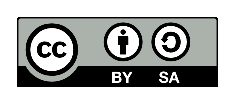
\includegraphics[scale=0.5]{img/cc-by-sa_88x31}} \par
	{\footnotesize{This work is licensed under the Creative Commons Attribution-ShareAlike 4.0 International License. To view a copy of this license, visit \href{http://creativecommons.org/licenses/by-sa/4.0/}{http://creativecommons.org/licenses/by-sa/4.0/} or send a letter to Creative Commons, PO Box 1866, Mountain View, CA 94042, USA.}}\par
\medskip
\qrcode[hyperlink,height=1.5cm]{http://creativecommons.org/licenses/by-sa/4.0/}
\end{center}
\vspace*{\stretch{1}}
\newpage
 % Licence page
\vspace*{\stretch{5}}
\section*{Preface}
The primary aim of this project is to create a printable guitar chords booklet for everyone.\par
\medskip
This booklet provides a lot of possibilities: you can update it with new songs without reprinting the whole book,
you can share this booklet with your friends, you can use it for bringing the music to every street of the world, or rather, you can become a GuitarHub hero.\par
\medskip
Thank you for using this booklet.\par
\smallskip
Thank you for sharing it.\par
\smallskip
Thank you for becoming a GuitarHub hero.\par
\bigskip
\begin{flushright}
	{\small{\textit{The first author of this booklet,}}}\par
	\medskip
	{\large{\textit{\rmfamily Pietro Prandini}}}\par
\end{flushright}
\vspace*{\stretch{12}}
\newpage

% Copyright 2018-2021 Pietro Prandini
% 
% This file is part of GuitarHub.
% 
% GuitarHub is free software: you can redistribute it and/or modify
% it under the terms of the GNU General Public License as published by
% the Free Software Foundation, either version 3 of the License, or
% (at your option) any later version.
% 
% GuitarHub is distributed in the hope that it will be useful,
% but WITHOUT ANY WARRANTY; without even the implied warranty of
% MERCHANTABILITY or FITNESS FOR A PARTICULAR PURPOSE.  See the
% GNU General Public License for more details.
% 
% You should have received a copy of the GNU General Public License
% along with GuitarHub.  If not, see <https://www.gnu.org/licenses/>.

\section*{Considerations}
This book is meant mainly for the guitar players who would like to have a chords book that is updated periodically without the loss of formatting and any other related problems.\par
It is highly recommended to print the content of this booklet and put it in a ring notebook - when a new song is added you can print it out and place it in a desired location. In order to avoid inconsistencies when adding the new songs to your collection, the pages are not labeled with any numbers. You can, for example, order the songs alphabetically.\par

\section*{Features}
\begin{itemize}
\item The booklet is available to be printed at once, including all the songs till date and then you can expand it by adding the newly released songs without the necessity to reprint the whole booklet;
\item the format of a single page is ISO A5 which supports the idea of  portability;
\item each song starts at a page with an even number to support the updating process;
\item creating songs with musical note names in both absolute and solfege systems;
\item easy and automatic transposition of the chords;
\item ability to add your favourite songs;
\item the book is licensed by a Free Culture License;
\item support for creating songs;
\item support for generating the booklets.
\end{itemize}

\section*{How to have a copy}
See \href{https://github.com/PietroPrandini/GuitarHub}{https://github.com/PietroPrandini/GuitarHub}

\begin{center}
  \qrcode[hyperlink,height=1.5cm]{https://github.com/PietroPrandini/GuitarHub}
\end{center}


%	Indexes
\checkodd
%\showindex[2]{Chords}{chords}
%\showindex[2]{Canti per la Liturgia, per le Celebrazioni e per la Preghiera}{chiesa}
%\showindex[2]{Jukebox}{jukebox}
%\showindex[2]{Christmas}{christmas}

%	Showing the lists of the songs
%{\makeatletter\def\SB@ellipspread#1#2{\begin{flushleft}- #1\par\end{flushleft}}\showindex[2]{Chords}{chords}}
{\makeatletter\def\SB@ellipspread#1#2{- #1\hspace*{\fill}\par}\showindex[2]{Canti per la Liturgia, per le Celebrazioni e per la Preghiera\\\tiny{\filemodprintdate{"tex/songsChapters/chiesa.tex"}}}{chiesa}}
{\makeatletter\def\SB@ellipspread#1#2{- #1\hspace*{\fill}\par}\showindex[2]{Jukebox\\\tiny{\filemodprintdate{"tex/songsChapters/jukebox.tex"}}}{jukebox}}
{\makeatletter\def\SB@ellipspread#1#2{- #1\hspace*{\fill}\par}\showindex[2]{Christmas\\\tiny{\filemodprintdate{"tex/songsChapters/christmas.tex"}}}{christmas}}
\ifchorded
%	New chapter
%	Start on a right page and the title is in a blank page
\checkodd
\vspace*{\stretch{3}}
\songchapter{Chords}
\vspace*{\stretch{5}}
\newpage
%	Songs of this chapter
\songpos{0}
\begin{songs}{chords}
	\scleardpage
% Copyright 2018-2021 Pietro Prandini
% 
% This file is part of GuitarHub.
% 
% GuitarHub is free software: you can redistribute it and/or modify
% it under the terms of the GNU General Public License as published by
% the Free Software Foundation, either version 3 of the License, or
% (at your option) any later version.
% 
% GuitarHub is distributed in the hope that it will be useful,
% but WITHOUT ANY WARRANTY; without even the implied warranty of
% MERCHANTABILITY or FITNESS FOR A PARTICULAR PURPOSE.  See the
% GNU General Public License for more details.
% 
% You should have received a copy of the GNU General Public License
% along with GuitarHub.  If not, see <https://www.gnu.org/licenses/>.

\beginsong{Common chords}[
,cr={\centering{\href{https://github.com/PietroPrandini/GuitarHub}{https://github.com/PietroPrandini/GuitarHub}\\\href{http://creativecommons.org/licenses/by-sa/4.0/}{\textbf{CC BY-SA}} 2018-2021 Pietro Prandini}}, % Copyright information
]

\textnote{Common major chords}
\begin{center}
\gtab{A}{X02220:002340}
\gtab{A#/B&}{(X13331):112341}
\gtab{B}{(X24442):112341}
\gtab{C}{X32010:032010}
\gtab{C#/D&}{4:(X13331):112341}
\gtab{D}{XX0232:000132}
\gtab{D#/E&}{6:(X13331):112341}
\gtab{E}{022100:023100}
\gtab{F}{(133211):134211}
\gtab{F#/G&}{(244322):134211}
\gtab{G}{320033:210034}
\gtab{G#/A&}{4:(133211):134211}
\end{center}

\textnote{Common minor chords}
\begin{center}
\gtab{Am}{X02210:002310}
\gtab{A#m/B&m}{(X13321):113421}
\gtab{Bm}{(X24432):113421}
\gtab{Cm}{3:(X13321):113421}
\gtab{C#m/D&m}{4:(X13321):113421}
\gtab{Dm}{XX0231:000241}
\gtab{D#m/E&m}{6:(X13321):113421}
\gtab{Em}{022000:023000}
\gtab{Fm}{(133111):134111}
\gtab{F#m/G&m}{(244222):134111}
\gtab{Gm}{3:(133111):134111}
\gtab{G#m/A&m}{4:(133111):134111}
\end{center}

\endsong


\end{songs}
\songpos{3}
\fi

%	New chapter
%	Start on a right page and the title is in a blank page
\checkodd
\vspace*{\stretch{3}}
\songchapter{Canti per la Liturgia, per le Celebrazioni e per la Preghiera}
\vspace*{\stretch{5}}
\newpage
%	Songs of this chapter
\begin{songs}{chiesa}
	%	Songs of the chiesa chapter
% Copyright 2018-2023 Pietro Prandini
% 
% This file is part of GuitarHub.
% 
% GuitarHub is free software: you can redistribute it and/or modify
% it under the terms of the GNU General Public License as published by
% the Free Software Foundation, either version 3 of the License, or
% (at your option) any later version.
% 
% GuitarHub is distributed in the hope that it will be useful,
% but WITHOUT ANY WARRANTY; without even the implied warranty of
% MERCHANTABILITY or FITNESS FOR A PARTICULAR PURPOSE.  See the
% GNU General Public License for more details.
% 
% You should have received a copy of the GNU General Public License
% along with GuitarHub.  If not, see <https://www.gnu.org/licenses/>.

\ifchorded

\beginverse* 
{\nolyrics Intro: \[B] \[E] \[B] \[E]}
\endverse

\fi

\beginverse\memorize 
\[B]Dopo il tempo del deserto,
adesso è il \[E]tempo di pianure fertili.
\[B]Dopo il tempo delle nebbie,
adesso \[E]s'apre l'orizzonte limpido.
\[C#m]Dopo il tempo dell'attesa,
adesso è il \[G#m]canto, la pienezza \[F#]della gioia:
\[E] l'immacolata Donna ha \[F#]dato al mondo Dio.
\endverse

\beginverse
^La fanciulla più nascosta
adesso è ^madre del Signore Altissimo.
^La fanciulla più soave
adesso il^lumina la terra e i secoli.
^La fanciulla del silenzio
adesso è il ^canto, la pienezza ^della gioia:
^ l'immacolata Donna ha ^dato al mondo Dio.
\endverse

\beginchorus
È \[G#m]nato, nato!
\[B]È qualcosa di impen\[F#]sabile, eppure è \[G#m]nato, nato!
\[B]Noi non siamo soli, il Si\[F#]gnore ci è a fianco.
\[C#m] È \[E]nato!
\[B]Questa valle torne\[F#]rà come un giardino.
Il \[C#m]cuore già lo \[E]sa.
È \[B]nata la speranza. È \[F#]nata la speranza.
\endchorus

\beginverse
^La potenza del creato
adesso è il ^pianto di un bambino fragile.
^La potenza della gloria
adesso ^sta in una capanna povera.
^La potenza dell'amore
adesso è il ^canto, la pienezza ^della gioia:
^ l'immacolata Donna ha ^dato al mondo Dio.
\endverse

\beginverse
\[B]Tu adesso \[E]sei bimbo,
\[B]tu adesso \[E]hai una \[C#m]madre.
Tu l'hai cre\[G#m]ata bel\[E]lissima
e \[F#]dormi nel suo grembo.
\endverse


\ifchorded
	\input{"tex/songsChapters/chiesa/Adesso e la pienezza -2.tex"}
\fi
\input{"tex/songsChapters/chiesa/Adoro Te"}
% Copyright 2018-2022 Pietro Prandini
% 
% This file is part of GuitarHub.
% 
% GuitarHub is free software: you can redistribute it and/or modify
% it under the terms of the GNU General Public License as published by
% the Free Software Foundation, either version 3 of the License, or
% (at your option) any later version.
% 
% GuitarHub is distributed in the hope that it will be useful,
% but WITHOUT ANY WARRANTY; without even the implied warranty of
% MERCHANTABILITY or FITNESS FOR A PARTICULAR PURPOSE.  See the
% GNU General Public License for more details.
% 
% You should have received a copy of the GNU General Public License
% along with GuitarHub.  If not, see <https://www.gnu.org/licenses/>.

\beginchorus
\[C]Alle\[F]luia, alleluia,
\[C]alle\[G]luia, alleluia.
\[C]Alle\[F]luia, alleluia,
\[C]al\[G]lelu\[C]ia. \rep{2}
\endchorus

\beginverse*\memorize 
\[C]La Tua \[F]festa non \[G]deve \[C]finire,
non \[Am]deve fi\[Dm]nire e \[G]non fini\[C]rà.
\[C]La Tua \[F]festa non \[G]deve \[C]finire,
non \[Am]deve fi\[Dm]nire e \[G]non fini\[C]rà. \[C7]
Per\[F]chè la \[G]festa \[C]siamo \[Am]noi
che \[F]cammi\[G]niamo verso \[C]Te, \[C7]
per\[F]chè la \[G]festa \[C]siamo \[Am]noi
can\[D7]tando insieme co\[G4]sì. \[G]
\endverse


% Copyright 2018-2021 Pietro Prandini
% 
% This file is part of GuitarHub.
% 
% GuitarHub is free software: you can redistribute it and/or modify
% it under the terms of the GNU General Public License as published by
% the Free Software Foundation, either version 3 of the License, or
% (at your option) any later version.
% 
% GuitarHub is distributed in the hope that it will be useful,
% but WITHOUT ANY WARRANTY; without even the implied warranty of
% MERCHANTABILITY or FITNESS FOR A PARTICULAR PURPOSE.  See the
% GNU General Public License for more details.
% 
% You should have received a copy of the GNU General Public License
% along with GuitarHub.  If not, see <https://www.gnu.org/licenses/>.

\ifchorded

\beginverse* 
{\nolyrics Intro: \[D] \[A] \rep{2}}
\endverse

\fi

\beginchorus
\[D]Alle\[A]luia, \[F#m]
\[Bm]alleluia, \[F#m]alleluia,
\[G]alleluia, \[D]allelu\[Em]ia, \[A]
\[D]alle\[G]luia, al\[A]lelu\[D]ia.
\endchorus

\beginverse*
\[D]Passeranno i \[A]cieli \[F#m]
e \[Bm]passerà la \[F#m]terra,
\[G]la Sua Parola \[D]non passe\[Em]rà, \[A]
\[D]alle\[G]luia, al\[A]lelu\[D]ia.
\endverse


\beginsong{Alleluia questa Tua parola}[
,cr={\centering{\href{https://github.com/PietroPrandini/GuitarHub}{https://github.com/PietroPrandini/GuitarHub} - \href{http://creativecommons.org/licenses/by-sa/4.0/}{CC-BY-SA} - \filemodprintdate{"tex/chiesa/Alleluia questa Tua parola.tex"}}}, % Copyright information
]
\transpose{0}
%{\nolyrics Intro: }

\ifchorded
\beginverse*
{\nolyrics Intro: \[D] \[Em] \[G] \[D]}
\endverse
\fi

\beginchorus
\[D]Alleluia, \[A]Alleluia, \[Bm]Alleluia, A\[F#]lleluia,
\[G]Alleluia, \[D]Alleluia, \[E]Alleluia, A\[A4]lle\[A]luia.
\[D]Alleluia, \[A]Alleluia, \[Bm]Alleluia, A\[F#]lleluia,
\[G]Alleluia, \[D]Alleluia, \[E]Alleluia, A\[A4]lle\[A]lui\[D]a.
\endchorus

\beginverse*
\[D]Questa Tua parola \[C]non avr\`a mai fine,
\[G]ha varcato i cieli e \[D]porter\`a i suoi frutti.
\[D]Questa Tua parola \[C]non avr\`a mai fine,
\[G]ha varcato i cieli e \[A4]porter\`a i suoi \[A7]frutti.
\endverse

\beginchorus
\[D]Alleluia, \[A]Alleluia, \[Bm]Alleluia, A\[F#]lleluia,
\[G]Alleluia, \[D]Alleluia, \[E]Alleluia, A\[A4]lle\[A]lui\[D]a.
\endchorus

\endsong

%\meter{4}{4}

%	\ifchorded
%	\beginverse* % * not count the verse
%		{\nolyrics Intro: }
%	\endverse
%	\fi

	\beginchorus
		%chorus
		\[F]Alle\[C]luia, ser\[B&]vire \[C]è,
		\[F]alle\[C]luia, ser\[B&]vire è \[C]gioia.
		\[F]Alle\[C]luia, ser\[B&]vire \[C]è,
		\[F]alle\[C]luia, è \[B&]stare con \[C]Te, Ge\[F]sù. \[C] \[B&] \[C]
	\endchorus

	\beginverse\memorize % \memorize is used to set the chords you would like to use with ^ in the next verses
		%verse
		\[F]Come l'amico più \[C]grande \[B&]tu guidi i miei \[F]passi,
		\[F]sei lungo la \[C]strada \[B&]e cammini con \[C]me.
	\endverse

	\beginverse
		^Tu sai accogliere ^tutti, ^Tu sai donare spe^ranza,
		^hai parole d'a^more, ^voglio restare con ^Te.
	\endverse

	\beginverse
		^Costruirò la mia ^casa ^su una roccia si^cura,
		^sei la perla pre^ziosa, ^sei un tesoro per ^me.
	\endverse

	\beginverse
		^Hai detto: voi siete la ^luce, ^siete granelli di ^sale
		^e non abbiate pa^ura: ^non vi abbandone^rò.
	\endverse

%	\ifchorded
%	\beginverse* % * not count the verse
%		{\nolyrics Strum: }
%	\endverse
%	\fi

%	\textnote{} % Notes for both lyric and chorded songs
%	\musicnote{} % Notes visible only in chorded books (not visible in lyric mode)
%	\rep{n} % Repeat n times
%	\lrep ... \rrep \rep{n} % margins of the repeat

%	Writing chords
%
% Alphabetic note names:     A      B      C      D      E      F      G
% Solfedge note names:       LA     SI     DO     RE     MI     FA     SOL
%
%	Compatible notation:
%
% Naturals:                  \[A]   \[B]   \[C]   \[D]   \[E]   \[F]   \[G]
% Flat (Bemolle):            \[A&]  \[B&]  \[C&]  \[D&]  \[E&]  \[F&]  \[G&]
% Sharp (Diesis):            \[A#]  \[B#]  \[C#]  \[D#]  \[E#]  \[F#]  \[G#]
% Minor:                     \[Am]  \[Bm]  \[Cm]  \[Dm]  \[Em]  \[Fm]  \[Gm]
% Flat and minor:            \[A&m] \[B&m] \[C&m] \[D&m] \[E&m] \[F&m] \[G&m]
% Sharp and minor:           \[A#m] \[B#m] \[C#m] \[D#m] \[E#m] \[F#m] \[G#m]

% Copyright 2018-2022 Pietro Prandini
% 
% This file is part of GuitarHub.
% 
% GuitarHub is free software: you can redistribute it and/or modify
% it under the terms of the GNU General Public License as published by
% the Free Software Foundation, either version 3 of the License, or
% (at your option) any later version.
% 
% GuitarHub is distributed in the hope that it will be useful,
% but WITHOUT ANY WARRANTY; without even the implied warranty of
% MERCHANTABILITY or FITNESS FOR A PARTICULAR PURPOSE.  See the
% GNU General Public License for more details.
% 
% You should have received a copy of the GNU General Public License
% along with GuitarHub.  If not, see <https://www.gnu.org/licenses/>.

\beginverse\memorize 
Si\[A]gnore, sei ve\[C#m]nuto fra\[D]tello in mezzo a \[E]noi.
Si\[F#m]gnore, hai por\[D]tato \[B]amore e liber\[E]tà.
Si\[F#m]gnore, sei vissuto \[E]nella \[D]pover\[C#m]tà:
\[A]noi ti ringra\[D]ziamo Ge\[E]sù.
\endverse

\beginchorus
\[A]Alle\[F#m]luia, \[D] allelu\[E]ia, \[A]alle\[F#m]luia, \[B] allelu\[E]ia,
\[A]alle\[F#m]luia, \[D] allelu\[E]ia, \[C#m]alle\[D]lu\[A]ia. \[D] \[A]
\endchorus

\beginverse
Si^gnore, sei ve^nuto fra^tello nel do^lore.
Si^gnore, hai par^lato del ^regno dell'a^more.
Si^gnore, hai donato ^la tua ^vita a ^noi:
^noi ti ringra^ziamo Ge^sù.
\endverse


\ifchorded
	\input{"tex/songsChapters/chiesa/Alleluia Signore sei venuto -2.tex"}
\fi
% Copyright 2018-2021 Pietro Prandini
% 
% This file is part of GuitarHub.
% 
% GuitarHub is free software: you can redistribute it and/or modify
% it under the terms of the GNU General Public License as published by
% the Free Software Foundation, either version 3 of the License, or
% (at your option) any later version.
% 
% GuitarHub is distributed in the hope that it will be useful,
% but WITHOUT ANY WARRANTY; without even the implied warranty of
% MERCHANTABILITY or FITNESS FOR A PARTICULAR PURPOSE.  See the
% GNU General Public License for more details.
% 
% You should have received a copy of the GNU General Public License
% along with GuitarHub.  If not, see <https://www.gnu.org/licenses/>.

%\meter{4}{4}

	\ifchorded
	\beginverse* % * not count the verse
		{\nolyrics Intro: \[G] \[D] \[C] \[D]}
	\endverse
	\fi

	\beginchorus
		\[G]Alleluia, \[D]alleluia, \[C]allelu\[G]ia!
		\[Am]Una luce \[G]splendida \[C]illumina la \[G]ter\[D]ra.
		\[G]Alleluia, \[D]alleluia, \[C]allelu\[G]ia!
		\[Am]Dio si è fatto \[G]uomo, è ve\[C]nuto in mezzo a \[G]noi.
	\endchorus

	\beginchorus
		\textnote{Ending}
		Alle\[Am]luia, \[D]allelu\[G]ia! \[C] \[G]
	\endchorus

	\beginverse\memorize % \memorize is used to set the chords you would like to use with ^ in the next verses
		%verse
		È spun\[G]tato per il \[D]mondo un giorno \[C]san\[D]to,
		Ado\[G]riamo il si\[D]gnore, il dio bam\[C]bi\[F#]no.
		Ascol\[Em]tiamo la sua voce, acco\[Am]gliamo la sua \[B]pace.
		Dentro il \[C]cuore di ogni \[G]uomo il suo \[Am]amore reste\[D]rà.
	\endverse

	\beginverse
		È ve^nuta sulla ^terra la sua pa^ro^la,
		e per ^noi la sua sa^pienza si è fatta ^car^ne.
		Lui ci ^dona la sua luce, che ri^splende nella ^notte
		e ci ^guida nella ^vita cammi^nando insieme a ^noi.
	\endverse

%	\beginchorus
		%chorus
%	\endchorus

%	\ifchorded
%	\beginverse* % * not count the verse
%		{\nolyrics Strum: }
%	\endverse
%	\fi

%	\textnote{} % Notes for both lyric and chorded songs
%	\musicnote{} % Notes visible only in chorded books (not visible in lyric mode)
%	\rep{n} % Repeat n times
%	\lrep ... \rrep \rep{n} % margins of the repeat

%	Writing chords
%
% Alphabetic note names:     A      B      C      D      E      F      G
% Solfedge note names:       LA     SI     DO     RE     MI     FA     SOL
%
%	Compatible notation:
%
% Naturals:                  \[A]   \[B]   \[C]   \[D]   \[E]   \[F]   \[G]
% Flat (Bemolle):            \[A&]  \[B&]  \[C&]  \[D&]  \[E&]  \[F&]  \[G&]
% Sharp (Diesis):            \[A#]  \[B#]  \[C#]  \[D#]  \[E#]  \[F#]  \[G#]
% Minor:                     \[Am]  \[Bm]  \[Cm]  \[Dm]  \[Em]  \[Fm]  \[Gm]
% Flat and minor:            \[A&m] \[B&m] \[C&m] \[D&m] \[E&m] \[F&m] \[G&m]
% Sharp and minor:           \[A#m] \[B#m] \[C#m] \[D#m] \[E#m] \[F#m] \[G#m]

\ifchorded
	\input{"tex/songsChapters/chiesa/Alleluia una luce splendida -2.tex"}
\fi
%	\beginverse* % * not count the verse
%		{\nolyrics Intro: }
%	\endverse

%	\beginverse\memorize % \memorize is used to set the chords you would like to use with ^ in the next verses
		%verse
%	\endverse
	\meter{4}{4}
	\beginchorus
		%chorus
		|\[Bm]Alle\[A]lu\[D]ia alle\[Em]lui\[A]a
		\[Bm]alle\[A]lu\[D]ia alle\[Em]l\[F#m]u\[Bm]ia \rep{2}
	\endchorus

	\beginverse*
	\meter{2}{4}|\[Bm] Alleluia allelu\meter{4}{4}|ia all\[A]eluia \[Bm] all\[A]eluia|
		\[Em] all\[F#m]eluia \echo{\[G]all\[A]eluia}|
	\meter{2}{4}|\[Bm] Alleluia all\[A]elu\meter{4}{4}|\[Bm]ia all\[A]eluia \[Bm] all\[A]eluia|
		\[Em] all\[F#m]eluia \echo{\[G]all\[A]eluia}|
	\endverse

%	\textnote{} % Notes for both lyric and chorded songs
%	\musicnote{} % Notes visible only in chorded books (not visible in lyric mode)
%	\rep{n} % Repeat n times

%	Writing chords
%
% Alphabetic note names:     A      B      C      D      E      F      G
% Solfedge note names:       LA     SI     DO     RE     MI     FA     SOL
%
%	Compatible notation:
%
% Naturals:                  \[A]   \[B]   \[C]   \[D]   \[E]   \[F]   \[G]
% Flat (Bemolle):            \[A&]  \[B&]  \[C&]  \[D&]  \[E&]  \[F&]  \[G&]
% Sharp (Diesis):            \[A#]  \[B#]  \[C#]  \[D#]  \[E#]  \[F#]  \[G#]
% Minor:                     \[Am]  \[Bm]  \[Cm]  \[Dm]  \[Em]  \[Fm]  \[Gm]
% Flat and minor:            \[A&m] \[B&m] \[C&m] \[D&m] \[E&m] \[F&m] \[G&m]
% Sharp and minor:           \[A#m] \[B#m] \[C#m] \[D#m] \[E#m] \[F#m] \[G#m]

\beginsong{%Titles
Benedici o Signore}[
%by={},%authors, composers, and other contributors
,cr={\centering{\href{https://github.com/PietroPrandini/GuitarHub}{https://github.com/PietroPrandini/GuitarHub} - \href{http://creativecommons.org/licenses/by-sa/4.0/}{CC-BY-SA} - \filemodprintdate{"tex/songsBodies/Benedici o Signore.tex"}}}, % Copyright information
%sr={},%related scripture references
%index={},%an extra index entry for a line of lyrics
%ititle={}%an extra index entry for a hidden title
]

%\capo{0}
\transpose{0}

\beginsong{%Titles
Benedici o Signore}[
%by={},%authors, composers, and other contributors
,cr={\centering{\href{https://github.com/PietroPrandini/GuitarHub}{https://github.com/PietroPrandini/GuitarHub} - \href{http://creativecommons.org/licenses/by-sa/4.0/}{CC-BY-SA} - \filemodprintdate{"tex/songsBodies/Benedici o Signore.tex"}}}, % Copyright information
%sr={},%related scripture references
%index={},%an extra index entry for a line of lyrics
%ititle={}%an extra index entry for a hidden title
]

%\capo{0}
\transpose{0}

\input{"tex/songsBodies/Benedici o Signore.tex"}

\endsong


\endsong

\ifchorded
	\beginsong{%Titles
Benedici o Signore
}[
%by={},%authors, composers, and other contributors
%cr={},%copyright information
%li={},%licensing information
%sr={},%related scripture references
%index={V1},%an extra index entry for a line of lyrics
%ititle={V1}%an extra index entry for a hidden title
]

\capo{1}
\transpose{9}

\ifchorded
  \beginverse* % * not count the verse
	  {\nolyrics Intro: \[Dm] \[C] \[B&] \[A]}
  \endverse
\fi
	\beginverse\memorize % \memorize is used to set the chords you would like to use with ^ in the next verses
	%verse
	\[Dm]Nebbia e freddo, giorni lunghi e \[C]amari,
	mentre il seme m\[Dm]uore.
	\[F]Poi il prodigio, antico e sempre \[C]nuovo
	del primo filo d'\[B&]erba... e nel \[F]vento
	dell'es\[C]tate ond\[Dm]eggiano le \[F]spighe:
	a\[C]vremo ancora \[A]pan\[D]e!
	\endverse

	\beginchorus
	%chorus
	\[G]Bened\[D]ici, \[G]o \[D]Signore \[C]questa o\[G]fferta
	che por\[A]tiamo a Te.
	\[G]Facci \[D]uno, \[Bm]come il \[F#m]Pane \[E]che anche \[G]oggi
	hai \[D]dato a noi.
	\endchorus
	
	\beginverse
	^Nei filari, dopo il lungo ^inverno,
	fremono le ^viti.
	^La rugiada avvolge nel si^lenzio
	i primi tralci ^verdi... Poi i ^colori
	dell'aut^unno, coi ^grappoli ^maturi:
	a^vremo ancora ^vi^no! 
	\endverse
% \textnote{} %for notes

%                 Do     Re     Mi     Fa     Sol    La     Si
%Naturali:        \[C]   \[D]   \[E]   \[F]   \[G]   \[A]   \[B]
%Bemolli:         \[C&]  \[D&]  \[E&]  \[F&]  \[G&]  \[A&]  \[B&]
%Diesis:          \[C#]  \[D#]  \[E#]  \[F#]  \[G#]  \[A#]  \[B#]
%Minori:          \[Cm]  \[Dm]  \[Em]  \[Fm]  \[Gm]  \[Am]  \[Bm]
%Bemolli minori:  \[C&m] \[D&m] \[E&m] \[F&m] \[G&m] \[A&m] \[B&m]
%Diesis minori:   \[C#m] \[D#m] \[E#m] \[F#m] \[G#m] \[A#m] \[B#m]

\endsong

\fi
\beginsong{%Title
Canto dell'Amore}[
%by={} % Authors, composers, and other contributors
%,cr={} % Copyright information
%,li={} % Licensing information
%,sr={} % Related scripture references
%,index={} % An extra index entry for a line of lyrics
%,ititle={} % An extra index entry for a hidden title
]

%\capo{0}
\transpose{0} % Automatic transpositions from +0 to +12 semitones

%	\beginverse* % * not count the verse
%		{\nolyrics Intro: }
%	\endverse

	\beginverse\memorize % \memorize is used to set the chords you would like to use with ^ in the next verses
		%verse
		Se \[E]dovrai attraversare il de\[C#m]serto
		non te\[A]mere Io sarò con \[E]te
		se dovrai camminare nel f\[C#m]uoco
		la sua f\[A]iamma non ti bruce\[E]rà
		segui\[B]rai la mia \[A]luce nella \[E]notte
		senti\[F#m]rai la mia \[B]forza nel camm\[C#m]ino
		io \[D]sono il tuo Dio, \[A] il Signore\[E]. \[C#m] \[A] \[E]
	\endverse

	\beginverse
		Sono ^Io che ti ho fatto e plas^mato
		ti ho ch^iamato per nome^
		Io da sempre ti ho conosc^iuto
		e ti ho ^dato il mio amore^
		perché ^tu sei pre^zioso ai miei oc^chi
		vali ^più del ^più grande dei te^sori
		Io ^sarò con te ^ dovunque and^rai. ^ ^ ^
	\endverse

	\ifchorded
	\beginverse*
		{\nolyrics Bridge \[B] \[A] \[E] \[D] \[A] \[B]}
	\endverse
	\fi

	\beginverse
		Non pen^sare alle cose di ^ieri
		cose n^uove fioriscono ^già
		aprirò nel deserto sent^ieri
		darò ^acqua nell'aridi^tà
		perché ^tu sei pre^zioso ai miei oc^chi
		vali ^più del ^più grande dei te^sori
		io ^sarò con te^ dovunque and^rai
		perché \[B]tu sei pre\[A]zioso ai miei oc\[E]chi
		vali \[F#m]più del \[B]più grande dei te\[C#m]sori
		io \[D]sarò con te \[A] dovunque and\[E]rai. \[C#m] \[A] \[E]
	\endverse

	\beginverse*
		Io ti sarò \[C#m] accanto \[A]sarò con \[E]te
		per tutto \[C#m] il tuo viaggio \[A]sarò con \[E]te. \rep{2}
	\endverse

%	\beginchorus
		%chorus
%	\endchorus

%	\textnote{} % Notes for both lyric and chorded songs
%	\musicnote{} % Notes visible only in chorded books (not visible in lyric mode)
%	\rep{n} % Repeat n times

%	Writing chords
%
% Alphabetic note names:     A      B      C      D      E      F      G
% Solfedge note names:       LA     SI     DO     RE     MI     FA     SOL
%
%	Compatible notation:
%
% Naturals:                  \[A]   \[B]   \[C]   \[D]   \[E]   \[F]   \[G]
% Flat (Bemolle):            \[A&]  \[B&]  \[C&]  \[D&]  \[E&]  \[F&]  \[G&]
% Sharp (Diesis):            \[A#]  \[B#]  \[C#]  \[D#]  \[E#]  \[F#]  \[G#]
% Minor:                     \[Am]  \[Bm]  \[Cm]  \[Dm]  \[Em]  \[Fm]  \[Gm]
% Flat and minor:            \[A&m] \[B&m] \[C&m] \[D&m] \[E&m] \[F&m] \[G&m]
% Sharp and minor:           \[A#m] \[B#m] \[C#m] \[D#m] \[E#m] \[F#m] \[G#m]

%	You can print the book with solfege note names
%	by uncomment a line of the GuitarChords.tex:
%	```
%	%\input{SolfedgeNoteNames.tex} % Solfedge note names
%	```

\endsong

\beginsong{%Title
Come ti ama Dio}[
%by={} % Authors, composers, and other contributors
,cr={\centering{\href{https://github.com/PietroPrandini/GuitarHub}{https://github.com/PietroPrandini/GuitarHub} \href{http://creativecommons.org/licenses/by-sa/4.0/}{CC-BY-SA} \filemodprintdate{"tex/chiesa/Come ti ama Dio.tex"}}}, % Copyright information
%,sr={} % Related scripture references
%,index={} % An extra index entry for a line of lyrics
%,ititle={} % An extra index entry for a hidden title
]

%\capo{0}
\transpose{0} % Automatic transpositions from +0 to +12 semitones

	\ifchorded
	\beginverse* % * not count the verse
		{\nolyrics Intro: \[D]\[Bm]\[G]\[A]}
	\endverse
	\fi

	\beginverse\memorize % \memorize is used to set the chords you would like to use with ^ in the next verses
		%verse
		\[D]Io vorrei sa\[Bm]perti amare \[G]come Dio,
		\[A] che ti prende per \[D]mano, ma ti \[Bm]lascia anche an\[G]dare;
		\[A]vorrei saperti a\[D]mare senza \[Bm]farti mai do\[G]mande
		\[A]felice perché e\[D]sisti
		e \[Bm]così io posso \[G]darti il \[A]meglio di \[D]me.
	\endverse

	\beginchorus
		%chorus
		Con la \[A]forza del \[Bm]mare, l'e\[G]ternità dei \[D]giorni,
		la \[A]gioia dei \[Bm]voli, la \[G]pace della \[D]sera,
		l'im\[A]mensità del \[Bm]cielo, \[G]come ti ama \[D]Dio. \[A]
	\endchorus

	\beginverse
		^Io vorrei sa^perti amare ^come Dio,
		^ che ti cono^sce e ti ac^cetta come ^sei,
		^tenerti tra le ^mani come i ^voli nell'az^zurro
		^felice perché e^sisti
		e ^così io posso ^darti il ^meglio di ^me.
	\endverse

	\beginverse
		^Io vorrei sa^perti amare ^come Dio
		^ che ti fa mi^gliore con l'a^more che ti ^dona
		^seguirti tra la ^gente con la ^gioia che hai ^dentro
		^felice perché e^sisti
		e ^così io posso ^darti il ^meglio di ^me.
	\endverse

%	\textnote{} % Notes for both lyric and chorded songs
%	\musicnote{} % Notes visible only in chorded books (not visible in lyric mode)
%	\rep{n} % Repeat n times

%	Writing chords
%
% Alphabetic note names:     A      B      C      D      E      F      G
% Solfedge note names:       LA     SI     DO     RE     MI     FA     SOL
%
%	Compatible notation:
%
% Naturals:                  \[A]   \[B]   \[C]   \[D]   \[E]   \[F]   \[G]
% Flat (Bemolle):            \[A&]  \[B&]  \[C&]  \[D&]  \[E&]  \[F&]  \[G&]
% Sharp (Diesis):            \[A#]  \[B#]  \[C#]  \[D#]  \[E#]  \[F#]  \[G#]
% Minor:                     \[Am]  \[Bm]  \[Cm]  \[Dm]  \[Em]  \[Fm]  \[Gm]
% Flat and minor:            \[A&m] \[B&m] \[C&m] \[D&m] \[E&m] \[F&m] \[G&m]
% Sharp and minor:           \[A#m] \[B#m] \[C#m] \[D#m] \[E#m] \[F#m] \[G#m]

%	You can print the book with solfege note names
%	by uncomment a line of the GuitarChords.tex:
%	```
%	%\input{SolfedgeNoteNames.tex} % Solfedge note names
%	```

\endsong

\ifchorded
	\input{"tex/songsChapters/chiesa/Come ti ama Dio v1.tex"}
\fi
% Copyright 2018-2021 Pietro Prandini
% 
% This file is part of GuitarHub.
% 
% GuitarHub is free software: you can redistribute it and/or modify
% it under the terms of the GNU General Public License as published by
% the Free Software Foundation, either version 3 of the License, or
% (at your option) any later version.
% 
% GuitarHub is distributed in the hope that it will be useful,
% but WITHOUT ANY WARRANTY; without even the implied warranty of
% MERCHANTABILITY or FITNESS FOR A PARTICULAR PURPOSE.  See the
% GNU General Public License for more details.
% 
% You should have received a copy of the GNU General Public License
% along with GuitarHub.  If not, see <https://www.gnu.org/licenses/>.

\ifchorded

  \beginverse* 
{\nolyrics Intro: \[E] \[G#m] \[A] \[B] \rep{2}}
  \endverse

\fi

\beginverse\memorize 
\[A]Tu ci raduni da ogni \[E]parte del mondo
noi si\[F#m]amo tuoi figli, tuo \[C#m]popolo san\[B]to.
\[A]Lodiamo in coro con le \[B]schiere ce\[C#m]lesti,
in\[D]sieme cantiamo, gio\[A]iosi accla\[B]miamo.
\endverse

\beginchorus
\[E]O Si\[B]gnore, ve\[A]niamo a \[B]Te,
    \[E]con i c\[B]uori ri\[A]colmi di \[A&]gioia,
    \[A]Ti \[B]ringraziamo per i \[F#m]doni che \[C#m]dai
    \[A]e per l'\[B]amore che riv\[F#m]ersi in no\[B]i.
    \[E]O Si\[B]gnore, ve\[A]niamo a \[A]Te,
    \[E]con i c\[B]uori ri\[A]colmi di \[A&]gioia,
    \[C#m]le nostre \[A&m]mani inna\[F#m]lziamo al \[C#m]cielo,
    \[A]a te con \[B]gioia ven\[E]iam. \[G#m] \[A] \[B]
  \endchorus

  \textnote{Ending: a te con gioia veniam (x3)}
\beginverse
  ^La Parola che ci ^doni Signore,
  ill^umina i cuori, ci ^mostra la ^via.
  ^Dove andremo se non ^resti con ^noi?
  Tu ^solo sei vita, ^tu sei veri^t\`a.
\endverse

\beginverse
^La grazia immensa che ci ^doni Signore
pur^ifica i cuori, con^sola i tuoi fi^gli.
^Nel tuo nome noi ^speriamo ^Signore
sal^vezza del mondo, ^eterno splen^dore.
\endverse


\ifchorded
	\beginsong{Con gioia veniamo a Te}[
%by={authors, composers, and other contributors},
,cr={\centering{\href{https://github.com/PietroPrandini/GuitarHub}{https://github.com/PietroPrandini/GuitarHub} \href{http://creativecommons.org/licenses/by-sa/4.0/}{CC-BY-SA} \filemodprintdate{"tex/chiesa/Con gioia veniamo a te -2.tex"}}}, % Copyright information
%li={licensing information},
%sr={related scripture references},
%index={an extra index entry for a line of lyrics},
%ititle={an extra index entry for a hidden title}
]

%\capo{0}
\transpose{10}

\ifchorded
  \beginverse* % * not count the verse
		{\nolyrics Intro: \[E] \[G#m] \[A] \[B] \rep{2}}
  \endverse
\fi
	\beginverse\memorize % \memorize is used to set the chords you would like to use with ^ in the next verses
		\[A]Tu ci raduni da ogni \[E]parte del mondo
		noi si\[F#m]amo tuoi figli, tuo \[C#m]popolo san\[B]to.
		\[A]Lodiamo in coro con le \[B]schiere ce\[C#m]lesti,
		in\[D]sieme cantiamo, gio\[A]iosi accla\[B]miamo.
	\endverse

	\beginchorus
		\[E]O Si\[B]gnore, ve\[A]niamo a \[B]Te,
    \[E]con i c\[B]uori ri\[A]colmi di \[A&]gioia,
    \[A]Ti \[B]ringraziamo per i \[F#m]doni che \[C#m]dai
    \[A]e per l'\[B]amore che riv\[F#m]ersi in no\[B]i.
    \[E]O Si\[B]gnore, ve\[A]niamo a \[A]Te,
    \[E]con i c\[B]uori ri\[A]colmi di \[A&]gioia,
    \[C#m]le nostre \[A&m]mani inna\[F#m]lziamo al \[C#m]cielo,
    \[A]a te con \[B]gioia ven\[E]iam. \[G#m] \[A] \[B]
  \endchorus
  \textnote{Ending: a te con gioia veniam (x3)}

	\beginverse
	  ^La Parola che ci ^doni Signore,
	  ill^umina i cuori, ci ^mostra la ^via.
	  ^Dove andremo se non ^resti con ^noi?
	  Tu ^solo sei vita, ^tu sei veri^t\`a.
	\endverse

	\beginverse
		^La grazia immensa che ci ^doni Signore
		pur^ifica i cuori, con^sola i tuoi fi^gli.
		^Nel tuo nome noi ^speriamo ^Signore
		sal^vezza del mondo, ^eterno splen^dore.
	\endverse

% \textnote{} %for notes

%                 Do     Re     Mi     Fa     Sol    La     Si
%Naturali:        \[C]   \[D]   \[E]   \[F]   \[G]   \[A]   \[B]
%Bemolli:         \[C&]  \[D&]  \[E&]  \[F&]  \[G&]  \[A&]  \[B&]
%Diesis:          \[C#]  \[D#]  \[E#]  \[F#]  \[G#]  \[A#]  \[B#]
%Minori:          \[Cm]  \[Dm]  \[Em]  \[Fm]  \[Gm]  \[Am]  \[Bm]
%Bemolli minori:  \[C&m] \[D&m] \[E&m] \[F&m] \[G&m] \[A&m] \[B&m]
%Diesis minori:   \[C#m] \[D#m] \[E#m] \[F#m] \[G#m] \[A#m] \[B#m]

\endsong

\fi
% Copyright 2018-2021 Pietro Prandini
% 
% This file is part of GuitarHub.
% 
% GuitarHub is free software: you can redistribute it and/or modify
% it under the terms of the GNU General Public License as published by
% the Free Software Foundation, either version 3 of the License, or
% (at your option) any later version.
% 
% GuitarHub is distributed in the hope that it will be useful,
% but WITHOUT ANY WARRANTY; without even the implied warranty of
% MERCHANTABILITY or FITNESS FOR A PARTICULAR PURPOSE.  See the
% GNU General Public License for more details.
% 
% You should have received a copy of the GNU General Public License
% along with GuitarHub.  If not, see <https://www.gnu.org/licenses/>.

\ifchorded

\beginverse* 
{\nolyrics Intro: \[F] \[C] \[B&] \[F] \[Gm] \[C]}
\endverse

\fi

\beginchorus
\[F]Con voce di giubilo \[B&]date il grande a\[C]nnuncio,
\[B&]fatelo g\[F]iungere ai con\[Gm]fini del \[C]mondo.
\[F]Con voce di giubilo \[B&]date il grande a\[C]nnuncio,
\[B&]il Signore ha libe\[F]rato il su\[Gm]o po\[C]po\[F]lo.
\endchorus

\beginverse\memorize 
Lo\[F]date il Signore egli \[Gm]è buono
Egli ha \[C]fatto \[B&]meravig\[F]lie, Alle\[Gm]lu\[C]ia
\endverse

\beginverse
Et^erna è la sua miseri^cordia
nel suo ^nome ^siamo ^salvi, alle^lu^ia
\endverse

\beginverse
La ^sua gloria riempie i cieli e la ^terra
è il Si^gnore ^della ^Vita, alle^lu^ia.
\endverse

\beginchorus
\[F]All\[B&]elu\[F]ia, \[F]All\[B&]elu\[F]ia, il Si\[B&]gnore ha libe\[F]rato il s\[Gm]uo p\[B&]opo\[C]lo.
\[F]All\[B&]elu\[F]ia, \[F]All\[B&]elu\[F]ia, il Si\[B&]gnore ha libe\[F]rato il s\[Gm]uo p\[B&]opo\[C]lo.
\[F]All\[B&]elu\[F]ia, \[F]All\[B&]elu\[F]ia!
\endchorus


\ifchorded
	\beginsong{%Title
Con voce di giubilo}[
%by={} % Authors, composers, and other contributors
,cr={\centering{\href{https://github.com/PietroPrandini/GuitarHub}{https://github.com/PietroPrandini/GuitarHub} \href{http://creativecommons.org/licenses/by-sa/4.0/}{CC-BY-SA} \filemodprintdate{"tex/chiesa/Con voce di giubilo -1.tex"}}}, % Copyright information
%,sr={} % Related scripture references
%,index={} % An extra index entry for a line of lyrics
%,ititle={} % An extra index entry for a hidden title
]

%\capo{0}
\transpose{11} % Automatic transpositions from +0 to +12 semitones

	\ifchorded
	\beginverse* % * not count the verse
		{\nolyrics Intro: \[F] \[C] \[B&] \[F] \[Gm] \[C]}
	\endverse
	\fi

	\beginchorus
		%chorus
		\[F]Con voce di giubilo \[B&]date il grande a\[C]nnuncio,
		\[B&]fatelo g\[F]iungere ai con\[Gm]fini del \[C]mondo.
		\[F]Con voce di giubilo \[B&]date il grande a\[C]nnuncio,
		\[B&]il Signore ha libe\[F]rato il su\[Gm]o po\[C]po\[F]lo.
	\endchorus

	\beginverse\memorize % \memorize is used to set the chords you would like to use with ^ in the next verses
		%verse
		Lo\[F]date il Signore egli \[Gm]è buono
		Egli ha \[C]fatto \[B&]meravig\[F]lie, Alle\[Gm]lu\[C]ia
	\endverse

	\beginverse
		Et^erna è la sua miseri^cordia
		nel suo ^nome ^siamo ^salvi, alle^lu^ia
	\endverse

	\beginverse
		La ^sua gloria riempie i cieli e la ^terra
		è il Si^gnore ^della ^Vita, alle^lu^ia.
	\endverse

	\beginchorus
		\[F]All\[B&]elu\[F]ia, \[F]All\[B&]elu\[F]ia, il Si\[B&]gnore ha libe\[F]rato il s\[Gm]uo p\[B&]opo\[C]lo.
		\[F]All\[B&]elu\[F]ia, \[F]All\[B&]elu\[F]ia, il Si\[B&]gnore ha libe\[F]rato il s\[Gm]uo p\[B&]opo\[C]lo.
		\[F]All\[B&]elu\[F]ia, \[F]All\[B&]elu\[F]ia!
	\endchorus

%	\textnote{} % Notes for both lyric and chorded songs
%	\musicnote{} % Notes visible only in chorded books (not visible in lyric mode)
%	\rep{n} % Repeat n times

%	Writing chords
%
% Alphabetic note names:     A      B      C      D      E      F      G
% Solfedge note names:       LA     SI     DO     RE     MI     FA     SOL
%
%	Compatible notation:
%
% Naturals:                  \[A]   \[B]   \[C]   \[D]   \[E]   \[F]   \[G]
% Flat (Bemolle):            \[A&]  \[B&]  \[C&]  \[D&]  \[E&]  \[F&]  \[G&]
% Sharp (Diesis):            \[A#]  \[B#]  \[C#]  \[D#]  \[E#]  \[F#]  \[G#]
% Minor:                     \[Am]  \[Bm]  \[Cm]  \[Dm]  \[Em]  \[Fm]  \[Gm]
% Flat and minor:            \[A&m] \[B&m] \[C&m] \[D&m] \[E&m] \[F&m] \[G&m]
% Sharp and minor:           \[A#m] \[B#m] \[C#m] \[D#m] \[E#m] \[F#m] \[G#m]

%	You can print the book with solfege note names
%	by uncomment a line of the GuitarChords.tex:
%	```
%	%\input{SolfedgeNoteNames.tex} % Solfedge note names
%	```

\endsong

\fi
% Copyright 2018-2021 Pietro Prandini
% 
% This file is part of GuitarHub.
% 
% GuitarHub is free software: you can redistribute it and/or modify
% it under the terms of the GNU General Public License as published by
% the Free Software Foundation, either version 3 of the License, or
% (at your option) any later version.
% 
% GuitarHub is distributed in the hope that it will be useful,
% but WITHOUT ANY WARRANTY; without even the implied warranty of
% MERCHANTABILITY or FITNESS FOR A PARTICULAR PURPOSE.  See the
% GNU General Public License for more details.
% 
% You should have received a copy of the GNU General Public License
% along with GuitarHub.  If not, see <https://www.gnu.org/licenses/>.

\meter{6}{8}

	\ifchorded
	\beginverse* % * not count the verse
		{\nolyrics Intro: | \[B&] \[F] | \[Gm] \[F] | \[E&] | \[F4] \[F] |}
	\endverse
	\fi

	\beginchorus
		%chorus
		Dal \[B&]tronco di \[F]Iesse \[E&]germoglie\[B&]rà
		un \[E&]nuovo vir\[B&]gulto do\[F]ma\[D]ni;
		dal\[Gm]le sue ra\[F]dici \[E&]si eleve\[B&]rà
		un \[Cm]albero \[F]nuo\[B&]vo. \rep{2}
	\endchorus

	\beginverse\memorize % \memorize is used to set the chords you would like to use with ^ in the next verses
		%verse
		Su di \[Gm]lui scende\[Dm]rà lo \[E&]Spirito di \[B&]Dio,
		gli \[Cm]regale\[Gm]rà i \[E&]suoi ricchi \[F]doni:
		con\[Gm]siglio e sa\[Dm]pienza, \[E&]scienza e for\[B&]tezza,
		\[Cm]santo ti\[E&]more di \[F]Dio.
	\endverse

	\beginverse
		Non ^giudiche^rà ^per le appa^renze,
		non ^decide^rà per ^sentito ^dire;
		ai ^poveri ^poi ^darà con lar^ghezza,
		fa^rà giu^stizia agli op^pressi.
	\endverse

	\beginverse
		Ed il ^lupo e l'a^gnello in ^pace vi^vranno,
		sa^ranno a^mici la ^mucca e il ^leone,
		^ed un fan^ciullo ^li guide^rà,
		^pascole^ranno in^sieme.
	\endverse

%	\ifchorded
%	\beginverse* % * not count the verse
%		{\nolyrics Strum: }
%	\endverse
%	\fi

%	\textnote{} % Notes for both lyric and chorded songs
%	\musicnote{} % Notes visible only in chorded books (not visible in lyric mode)
%	\rep{n} % Repeat n times
%	\lrep ... \rrep \rep{n} % margins of the repeat

%	Writing chords
%
% Alphabetic note names:     A      B      C      D      E      F      G
% Solfedge note names:       LA     SI     DO     RE     MI     FA     SOL
%
%	Compatible notation:
%
% Naturals:                  \[A]   \[B]   \[C]   \[D]   \[E]   \[F]   \[G]
% Flat (Bemolle):            \[A&]  \[B&]  \[C&]  \[D&]  \[E&]  \[F&]  \[G&]
% Sharp (Diesis):            \[A#]  \[B#]  \[C#]  \[D#]  \[E#]  \[F#]  \[G#]
% Minor:                     \[Am]  \[Bm]  \[Cm]  \[Dm]  \[Em]  \[Fm]  \[Gm]
% Flat and minor:            \[A&m] \[B&m] \[C&m] \[D&m] \[E&m] \[F&m] \[G&m]
% Sharp and minor:           \[A#m] \[B#m] \[C#m] \[D#m] \[E#m] \[F#m] \[G#m]

\ifchorded
	%	Uncomment the next two lines and the last twice
%	if the song is over 2 pages
%\renewcommand{\lyricfont}{\sffamily\small}
%\renewcommand{\printchord}[1]{\rmfamily\bf#1\small}

\beginsong{%Title
Dal tronco di Iesse}[
%by={} % Authors, composers, and other contributors
,cr={\centering{\href{https://github.com/PietroPrandini/GuitarHub}{https://github.com/PietroPrandini/GuitarHub} - \href{http://creativecommons.org/licenses/by-sa/4.0/}{CC-BY-SA} - \filemodprintdate{"tex/chiesa/Dal tronco di Iesse -1.tex"}}}, % Copyright information
%,li={} % Licensing information
%,sr={} % Related scripture references
%,index={} % An extra index entry for a line of lyrics
%,ititle={} % An extra index entry for a hidden title
]

%\capo{0}
\transpose{11} % Automatic transpositions from +0 to +12 semitones
\meter{6}{8}

	\ifchorded
	\beginverse* % * not count the verse
		{\nolyrics Intro: | \[B&] \[F] | \[Gm] \[F] | \[E&] | \[F4] \[F] |}
	\endverse
	\fi

	\beginchorus
		%chorus
		Dal \[B&]tronco di \[F]Iesse \[E&]germoglie\[B&]rà
		un \[E&]nuovo vir\[B&]gulto do\[F]ma\[D]ni;
		dal\[Gm]le sue ra\[F]dici \[E&]si eleve\[B&]rà
		un \[Cm]albero \[F]nuo\[B&]vo. \rep{2}
	\endchorus

	\beginverse\memorize % \memorize is used to set the chords you would like to use with ^ in the next verses
		%verse
		Su di \[Gm]lui scende\[Dm]rà lo \[E&]Spirito di \[B&]Dio,
		gli \[Cm]regale\[Gm]rà i \[E&]suoi ricchi \[F]doni:
		con\[Gm]siglio e sa\[Dm]pienza, \[E&]scienza e for\[B&]tezza,
		\[Cm]santo ti\[E&]more di \[F]Dio.
	\endverse

	\beginverse
		Non ^giudiche^rà ^per le appa^renze,
		non ^decide^rà per ^sentito ^dire;
		ai ^poveri ^poi ^darà con lar^ghezza,
		fa^rà giu^stizia agli op^pressi.
	\endverse

	\beginverse
		Ed il ^lupo e l'a^gnello in ^pace vi^vranno,
		sa^ranno a^mici la ^mucca e il ^leone,
		^ed un fan^ciullo ^li guide^rà,
		^pascole^ranno in^sieme.
	\endverse

%	\ifchorded
%	\beginverse* % * not count the verse
%		{\nolyrics Strum: }
%	\endverse
%	\fi

%	\textnote{} % Notes for both lyric and chorded songs
%	\musicnote{} % Notes visible only in chorded books (not visible in lyric mode)
%	\rep{n} % Repeat n times
%	\lrep ... \rrep \rep{n} % margins of the repeat

%	Writing chords
%
% Alphabetic note names:     A      B      C      D      E      F      G
% Solfedge note names:       LA     SI     DO     RE     MI     FA     SOL
%
%	Compatible notation:
%
% Naturals:                  \[A]   \[B]   \[C]   \[D]   \[E]   \[F]   \[G]
% Flat (Bemolle):            \[A&]  \[B&]  \[C&]  \[D&]  \[E&]  \[F&]  \[G&]
% Sharp (Diesis):            \[A#]  \[B#]  \[C#]  \[D#]  \[E#]  \[F#]  \[G#]
% Minor:                     \[Am]  \[Bm]  \[Cm]  \[Dm]  \[Em]  \[Fm]  \[Gm]
% Flat and minor:            \[A&m] \[B&m] \[C&m] \[D&m] \[E&m] \[F&m] \[G&m]
% Sharp and minor:           \[A#m] \[B#m] \[C#m] \[D#m] \[E#m] \[F#m] \[G#m]

\endsong

%\renewcommand{\lyricfont}{\sffamily}
%\renewcommand{\printchord}[1]{\rmfamily\bf#1}

\fi
% Copyright 2018-2024 Pietro Prandini
% 
% This file is part of GuitarHub.
% 
% GuitarHub is free software: you can redistribute it and/or modify
% it under the terms of the GNU General Public License as published by
% the Free Software Foundation, either version 3 of the License, or
% (at your option) any later version.
% 
% GuitarHub is distributed in the hope that it will be useful,
% but WITHOUT ANY WARRANTY; without even the implied warranty of
% MERCHANTABILITY or FITNESS FOR A PARTICULAR PURPOSE.  See the
% GNU General Public License for more details.
% 
% You should have received a copy of the GNU General Public License
% along with GuitarHub.  If not, see <https://www.gnu.org/licenses/>.

\ifchorded

\beginverse* 
{\nolyrics Intro: \[A] \[Bm] \[F#m] \[G] \[D] \[Em] \[D]}
\endverse

\fi

\beginchorus
\[D]Del tuo \[G]Spiri\[D]to, \[G]Signo\[D]re, \[A]\'e \[Bm]piena la \[F#m]terr\[G]a,
\'e \[D]piena la \[Em]terr\[D]a. \rep{2}
\endchorus

\beginverse\memorize
\[C]Benedici il Si\[B&]gnore,
\[Dm]anima \[Am]mi\[B&]a,
Si\[C]gnore, \[F]Dio\[C],
tu sei \[G]grand\[C]e!
\[C]Sono immense, splend\[B&]enti
\[Dm]tutte le Tue o\[B&]per\[F]e
e t\[Gm]utte le crea\[Gm]tur\[D]e.
\endverse

\beginverse
^Se tu togli il tuo ^soffio
^muore ogni ^cos^a
e ^si diss^olv^e
nella ^terr^a.
^Il tuo spirito ^scende
^tutto si ^ricre^a
e t^utto si ^rinnov^a.
\endverse

\beginverse
^La tua gloria, Si^gnore,
^resti per ^sempr^e.
Gio^isci, ^Di^o,
del cr^eat^o.
^Questo semplice ^canto
^salga a te Si^gnor^e
sei ^tu la nostra gi^oi^a.
\endverse


\beginsong{%Titles
\`E giunta l'ora}[
%by={}%authors, composers, and other contributors
%,cr={}%copyright information
%,li={}%licensing information
%,sr={}%related scripture references
%,index={}%an extra index entry for a line of lyrics
%,ititle={}%an extra index entry for a hidden title
]

%\capo{0}
\transpose{0}

%	\beginverse* % * not count the verse
%		{\nolyrics Intro: }
%	\endverse

%	\beginverse\memorize % \memorize is used to set the chords you would like to use with ^ in the next verses
		%verse
%	\endverse

%	\beginchorus
		%chorus
%	\endchorus

\beginverse\memorize
\`E giunta \[F]l’ora, \[B&]Padre, per \[F]me:
ai miei a\[Dm]mici \[B&] ho detto \[Gm]che \[C]
questa \`e la \[Am]vita: \[Dm]conoscere \[Am]Te
e \[B&]il Figlio \[C]Tuo: Cristo Ge\[F]s\`u. \[B&]\[F]
\endverse
\beginverse
Erano ^tuoi, ^li hai dati a ^me,
ed ora ^sanno ^che torno a ^Te.^
Hanno cre^duto: ^conservali ^Tu
nel ^tuo Am^ore, nell’uni^t\`a. ^^
\endverse
\beginverse
Tu mi hai ^mandato ^ai figli ^tuoi:
la tua ^parola ^\`e veri^t\`a.^
E il loro ^cuore ^sia pieno di gi^oia:
la ^gioia ^vera viene da ^Te.^^
\endverse
\beginverse
Io sono in ^loro e ^Tu in ^me;
e siam ^perfetti ^nell’uni^t\`a;^
e il mondo ^creda ^che Tu mi hai mand^ato:
li ^hai am^ati come ami ^me.^^
\endverse

%	\textnote{} %for notes

%                 Do     Re     Mi     Fa     Sol    La     Si
%Naturali:        \[C]   \[D]   \[E]   \[F]   \[G]   \[A]   \[B]
%Bemolli:         \[C&]  \[D&]  \[E&]  \[F&]  \[G&]  \[A&]  \[B&]
%Diesis:          \[C#]  \[D#]  \[E#]  \[F#]  \[G#]  \[A#]  \[B#]
%Minori:          \[Cm]  \[Dm]  \[Em]  \[Fm]  \[Gm]  \[Am]  \[Bm]
%Bemolli minori:  \[C&m] \[D&m] \[E&m] \[F&m] \[G&m] \[A&m] \[B&m]
%Diesis minori:   \[C#m] \[D#m] \[E#m] \[F#m] \[G#m] \[A#m] \[B#m]

\endsong

\beginsong{\`E Natale}[
by={Forza venite gente}
,cr={\centering{\href{https://github.com/PietroPrandini/GuitarHub}{https://github.com/PietroPrandini/GuitarHub}\\\href{http://creativecommons.org/licenses/by-sa/4.0/}{\textbf{CC BY-SA}} Pietro Prandini 2021}}, % Copyright information
%sr={related scripture references},
%index={an extra index entry for a line of lyrics},
%ititle={an extra index entry for a hidden title}
]
\transpose{0}

\beginsong{\`E Natale}[
by={Forza venite gente}
,cr={\centering{\href{https://github.com/PietroPrandini/GuitarHub}{https://github.com/PietroPrandini/GuitarHub}\\\href{http://creativecommons.org/licenses/by-sa/4.0/}{\textbf{CC BY-SA}} Pietro Prandini 2021}}, % Copyright information
%sr={related scripture references},
%index={an extra index entry for a line of lyrics},
%ititle={an extra index entry for a hidden title}
]
\transpose{0}

\input{"tex/songs/E Natale.tex"}

\endsong


\endsong

\ifchorded
	\beginsong{\`E Natale}[
by={Forza venite gente},
,cr={\centering{\href{https://github.com/PietroPrandini/GuitarHub}{https://github.com/PietroPrandini/GuitarHub} - \href{http://creativecommons.org/licenses/by-sa/4.0/}{CC-BY-SA} - \filemodprintdate{"tex/songsBodies/E Natale.tex"}}}, % Copyright information
%sr={related scripture references},
%index={an extra index entry for a line of lyrics},
%ititle={an extra index entry for a hidden title}
]
\transpose{10}

\beginsong{\`E Natale}[
by={Forza venite gente}
,cr={\centering{\href{https://github.com/PietroPrandini/GuitarHub}{https://github.com/PietroPrandini/GuitarHub}\\\href{http://creativecommons.org/licenses/by-sa/4.0/}{\textbf{CC BY-SA}} Pietro Prandini 2021}}, % Copyright information
%sr={related scripture references},
%index={an extra index entry for a line of lyrics},
%ititle={an extra index entry for a hidden title}
]
\transpose{0}

\input{"tex/songs/E Natale.tex"}

\endsong


\endsong

\fi
% Copyright 2018-2023 Pietro Prandini
% 
% This file is part of GuitarHub.
% 
% GuitarHub is free software: you can redistribute it and/or modify
% it under the terms of the GNU General Public License as published by
% the Free Software Foundation, either version 3 of the License, or
% (at your option) any later version.
% 
% GuitarHub is distributed in the hope that it will be useful,
% but WITHOUT ANY WARRANTY; without even the implied warranty of
% MERCHANTABILITY or FITNESS FOR A PARTICULAR PURPOSE.  See the
% GNU General Public License for more details.
% 
% You should have received a copy of the GNU General Public License
% along with GuitarHub.  If not, see <https://www.gnu.org/licenses/>.

\ifchorded

  \beginverse* 
  {\nolyrics Intro: \[C] \[B&] \[F] \[C7] x2}
  \endverse

\fi

\beginverse\memorize 
\[C]Scende il cielo sulla terra
sopra l'odio e sulla guerra
\[C7]scende il cielo e si fa storia
\[F]sfida il tempo e la memoria
\[C]ora \`e \[F] Natale an\[C]cora.
\endverse

\beginverse*
^Il passato \`e nel presente
nel futuro della gente
^e la pace \`e sempre un sogno
^dell'amore si ha bisogno
^ora \`e ^ Natale an^cora.
\endverse

\beginverse*
\[G]Ogni uomo pu\`o sentire
\[F]un segnale da seguire
\[C]ora \`e \[F] Natale an\[C]cora.
\endverse

\beginverse*
\[G]Ogni uomo qui nel mondo
\[F]una stella sta cercando
\[Dm]una luce \[Em]per torvare \[F]un po' di veri\[G]t\`a.
\endverse

\beginchorus
\[C]Merry Christmas all over the \[C7]world
\[F]nous chantons c'est Noel pour le \[Dm]monde
\[Am]buon Natale feliz \[Em]Navidad
\[F]per la pace \[Dm]che un giorno verr\`a\[G].
\[C]Merry Christmas all over the \[C7]world
\[F]c'est Noel non scordiamolo \[Dm]mai
\[Am]buon Natale feliz \[Em]Navidad
\[Fm]e la pace \[Dm]sia sempre con \[G]noi.
\ifchorded

  {\nolyrics \[C] \[B&] \[F] \[C7] \rep{2}}
\fi

\endchorus

  \beginverse
  \[C]Siamo popoli e nazioni
  secoli e generazioni
  \[C7]siamo figli del creato
  \[F]del presente e del passato
\[C]ora \`e \[F] Natale an\[C]cora.
  \endverse

  \beginverse*
  \[G]Nelle mani le bandiere
  \[F]nei paesi le frotiere
  \[Dm]ma nel cielo \[Em]il grido forte \[F]della liber\[G]t\`a.
  \endverse


% Copyright 2018-2021 Pietro Prandini
% 
% This file is part of GuitarHub.
% 
% GuitarHub is free software: you can redistribute it and/or modify
% it under the terms of the GNU General Public License as published by
% the Free Software Foundation, either version 3 of the License, or
% (at your option) any later version.
% 
% GuitarHub is distributed in the hope that it will be useful,
% but WITHOUT ANY WARRANTY; without even the implied warranty of
% MERCHANTABILITY or FITNESS FOR A PARTICULAR PURPOSE.  See the
% GNU General Public License for more details.
% 
% You should have received a copy of the GNU General Public License
% along with GuitarHub.  If not, see <https://www.gnu.org/licenses/>.

\beginverse\memorize 
\[D]Io lo so, Si\[F#m]gnore, che ve\[G]ngo da lon\[D]tano,
\[D]prima del pen\[F#m]siero e \[G]poi nella Tua m\[A]ano,
\[D]io mi rendo c\[A]onto che \[G]Tu sei la mia v\[D]ita
e \[G]non mi sembra \[Em]vero di preg\[E7]arti co\[A7]s\`i.
\endverse

\beginverse*
^"Padre d'ogni u^omo" e ^non Ti ho visto m^ai,
^"Spirito di ^vita" e ^nacqui da una don^na,
^"Figlio mio fra^tello" e ^sono solo un u^omo,
epp^ure io ca^pisco che ^Tu sei Ve^rit\`a.
\endverse

\beginchorus
E im\[D]parer\`o a gu\[G]ardare tutto \[A7]il mondo\[D7]
con gli \[G]occhi tra\[A]sparenti di un bam\[D]bino,
e ins\[G]egner\`o a chia\[A]marti "Pa\[D]dre n\[B7]ostro"
ad \[Em]ogni figlio \[E7]che diventa u\[A7]omo.
\endchorus

\beginchorus
E im\[D]parer\`o a gu\[G]ardare tutto \[A7]il mondo\[D7]
con gli \[G]occhi tra\[A]sparenti di un bam\[D]bino,
e ins\[G]egner\`o a chia\[A]marti "Pa\[D]dre n\[B7]ostro"
ad \[Em]ogni figlio c\[A7]he diventa u\[D]o\[G]mo.\[D]
\endchorus

\beginverse
^Io lo so, ^Signore, che ^tu mi sei vic^ino,
^luce alla mia ^mente, gu^ida al mio camm^ino,
^mano che sorr^egge, sgu^ardo che per^dona,
e ^non mi sembra ^vero che tu esista ^co^s\`i.
\endverse

\beginverse*
^Dove nasce ^amore ^Tu sei la sorg^ente,
^dove c'\`e una ^croce ^Tu sei la sper^anza,
^dove il tempo ^ha fine ^Tu sei vita et^erna:
e ^so che posso ^sempre contare ^su di^ Te!
\endverse

\beginchorus
E ac\[D]coglier\`o la \[G]vita \[A7]come un \[D7]dono,
e avr\`o \[G]il cor\[A]aggio di morire \[D]anch'io,
e in\[G]contro a te ver\[A]r\`o col \[D]mio fra\[B7]tello
che \[Em]non si s\[E7]ente amato da ne\[A]ssuno.
\endchorus

\beginchorus
E ac\[D]coglier\`o la \[G]vita \[A7]come un \[D7]dono,
e avr\`o \[G]il cor\[A]aggio di morire \[D]anch'io,
e in\[G]contro a te ver\[A]r\`o col \[D]mio fra\[B7]tello
che \[Em]non si \[A7]sente amato da \[D]ness\[G]uno.\[D]
\endchorus


% Copyright 2018-2021 Pietro Prandini
% 
% This file is part of GuitarHub.
% 
% GuitarHub is free software: you can redistribute it and/or modify
% it under the terms of the GNU General Public License as published by
% the Free Software Foundation, either version 3 of the License, or
% (at your option) any later version.
% 
% GuitarHub is distributed in the hope that it will be useful,
% but WITHOUT ANY WARRANTY; without even the implied warranty of
% MERCHANTABILITY or FITNESS FOR A PARTICULAR PURPOSE.  See the
% GNU General Public License for more details.
% 
% You should have received a copy of the GNU General Public License
% along with GuitarHub.  If not, see <https://www.gnu.org/licenses/>.

\beginchorus
\[C]Ecco\[G]mi, \[Dm]ecco\[Am]mi! \[F]Sig\[C]nore io \[G]vengo.
\[Am]Ecco\[Em]mi, \[F]ecco\[C]mi! \[F]Si compia in \[Am]me la tua\[G] volo\[C]nt\`a.
\endchorus

\beginverse\memorize
\[C]Nel mio Sig\[F]nore ho spe\[C]rato,
\[Am]e su di me s’\`e chi\[G]nato,
\[Dm]ha dato ascol\[G]to al mio g\[Am]rido,\[Em]
\[F]m’ha libera\[C]to dalla mort\[G]e.
\endverse

\beginverse
^I miei pi^edi ha reso s^aldi,
^sicuri ha reso i miei p^assi.
^Ha messo s^ulla mia ^boc^ca
^un nuovo ^canto di l^ode.
\endverse

\beginverse
^Il sacri^ficio non gradi^sci,
^ma m’hai aperto l’ore^cchio,
^non hai vol^uto olo^cau^sti,
^allora ho ^detto: io v^engo!
\endverse

\beginverse
^Sul tuo l^ibro di me \`e scr^itto:
^si compia il tuo v^olere.
^Questo mio ^Dio, de^sid^ero,
^la tua le^gge \`e nel mio c^uore.
\endverse

\beginverse
^La tua giu^stizia ho procl^amato,
^non tengo chiuse le l^abbra.
^Non rifi^utarmi, S^ign^ore,
^la tua ^misericor^dia.
\endverse


\ifchorded
	\beginsong{Eccomi}[
by={Frisina}
,cr={\centering{\href{https://github.com/PietroPrandini/GuitarHub}{https://github.com/PietroPrandini/GuitarHub} - \href{http://creativecommons.org/licenses/by-sa/4.0/}{CC-BY-SA} - \filemodprintdate{"tex/songs/Eccomi.tex"}}}, % Copyright information
]
\transpose{0}

% Copyright 2018-2021 Pietro Prandini
% 
% This file is part of GuitarHub.
% 
% GuitarHub is free software: you can redistribute it and/or modify
% it under the terms of the GNU General Public License as published by
% the Free Software Foundation, either version 3 of the License, or
% (at your option) any later version.
% 
% GuitarHub is distributed in the hope that it will be useful,
% but WITHOUT ANY WARRANTY; without even the implied warranty of
% MERCHANTABILITY or FITNESS FOR A PARTICULAR PURPOSE.  See the
% GNU General Public License for more details.
% 
% You should have received a copy of the GNU General Public License
% along with GuitarHub.  If not, see <https://www.gnu.org/licenses/>.

\beginchorus
\[C]Ecco\[G]mi, \[Dm]ecco\[Am]mi! \[F]Sig\[C]nore io \[G]vengo.
\[Am]Ecco\[Em]mi, \[F]ecco\[C]mi! \[F]Si compia in \[Am]me la tua\[G] volo\[C]nt\`a.
\endchorus

\beginverse\memorize
\[C]Nel mio Sig\[F]nore ho spe\[C]rato,
\[Am]e su di me s’\`e chi\[G]nato,
\[Dm]ha dato ascol\[G]to al mio g\[Am]rido,\[Em]
\[F]m’ha libera\[C]to dalla mort\[G]e.
\endverse

\beginverse
^I miei pi^edi ha reso s^aldi,
^sicuri ha reso i miei p^assi.
^Ha messo s^ulla mia ^boc^ca
^un nuovo ^canto di l^ode.
\endverse

\beginverse
^Il sacri^ficio non gradi^sci,
^ma m’hai aperto l’ore^cchio,
^non hai vol^uto olo^cau^sti,
^allora ho ^detto: io v^engo!
\endverse

\beginverse
^Sul tuo l^ibro di me \`e scr^itto:
^si compia il tuo v^olere.
^Questo mio ^Dio, de^sid^ero,
^la tua le^gge \`e nel mio c^uore.
\endverse

\beginverse
^La tua giu^stizia ho procl^amato,
^non tengo chiuse le l^abbra.
^Non rifi^utarmi, S^ign^ore,
^la tua ^misericor^dia.
\endverse



\endsong

	\beginsong{Eccomi}[
by={Frisina}
,cr={\centering{\href{https://github.com/PietroPrandini/GuitarHub}{https://github.com/PietroPrandini/GuitarHub} - \href{http://creativecommons.org/licenses/by-sa/4.0/}{CC-BY-SA} - \filemodprintdate{"tex/songs/Eccomi.tex"}}}, % Copyright information
]
\transpose{9}

% Copyright 2018-2021 Pietro Prandini
% 
% This file is part of GuitarHub.
% 
% GuitarHub is free software: you can redistribute it and/or modify
% it under the terms of the GNU General Public License as published by
% the Free Software Foundation, either version 3 of the License, or
% (at your option) any later version.
% 
% GuitarHub is distributed in the hope that it will be useful,
% but WITHOUT ANY WARRANTY; without even the implied warranty of
% MERCHANTABILITY or FITNESS FOR A PARTICULAR PURPOSE.  See the
% GNU General Public License for more details.
% 
% You should have received a copy of the GNU General Public License
% along with GuitarHub.  If not, see <https://www.gnu.org/licenses/>.

\beginchorus
\[C]Ecco\[G]mi, \[Dm]ecco\[Am]mi! \[F]Sig\[C]nore io \[G]vengo.
\[Am]Ecco\[Em]mi, \[F]ecco\[C]mi! \[F]Si compia in \[Am]me la tua\[G] volo\[C]nt\`a.
\endchorus

\beginverse\memorize
\[C]Nel mio Sig\[F]nore ho spe\[C]rato,
\[Am]e su di me s’\`e chi\[G]nato,
\[Dm]ha dato ascol\[G]to al mio g\[Am]rido,\[Em]
\[F]m’ha libera\[C]to dalla mort\[G]e.
\endverse

\beginverse
^I miei pi^edi ha reso s^aldi,
^sicuri ha reso i miei p^assi.
^Ha messo s^ulla mia ^boc^ca
^un nuovo ^canto di l^ode.
\endverse

\beginverse
^Il sacri^ficio non gradi^sci,
^ma m’hai aperto l’ore^cchio,
^non hai vol^uto olo^cau^sti,
^allora ho ^detto: io v^engo!
\endverse

\beginverse
^Sul tuo l^ibro di me \`e scr^itto:
^si compia il tuo v^olere.
^Questo mio ^Dio, de^sid^ero,
^la tua le^gge \`e nel mio c^uore.
\endverse

\beginverse
^La tua giu^stizia ho procl^amato,
^non tengo chiuse le l^abbra.
^Non rifi^utarmi, S^ign^ore,
^la tua ^misericor^dia.
\endverse



\endsong

\fi
% Copyright 2018-2024 Pietro Prandini
% 
% This file is part of GuitarHub.
% 
% GuitarHub is free software: you can redistribute it and/or modify
% it under the terms of the GNU General Public License as published by
% the Free Software Foundation, either version 3 of the License, or
% (at your option) any later version.
% 
% GuitarHub is distributed in the hope that it will be useful,
% but WITHOUT ANY WARRANTY; without even the implied warranty of
% MERCHANTABILITY or FITNESS FOR A PARTICULAR PURPOSE.  See the
% GNU General Public License for more details.
% 
% You should have received a copy of the GNU General Public License
% along with GuitarHub.  If not, see <https://www.gnu.org/licenses/>.

\meter{4}{4}

\ifchorded

\beginverse* 
{\nolyrics Intro: | \[G] \[D] | \[Em] \[G] | \[C] \[G] | \[D4] \[D] |}
\endverse

\fi

\beginverse\memorize 
\[G]Emmanu\[D]el, \[Em]tu sei qui con \[G]me,
\[C]vieni picco\[G]lissimo in\[Am]contro a \[D]me.
\[G]Emmanu\[D]el, a\[Em]mico silen\[Bm]zioso,
\[C]della tua pre\[G]senza riempi i \[Am]giorni \[D]miei.
\endverse

\beginchorus
\[G]Sei la \[D]luce \[C]dentro \[G]me,
\[C]sei la \[G]via da\[Am]vanti a \[D]me.
\[G]Nella \[D]storia ir\[B]rompi \[Em]tu,
\[G] \[C] io ti ac\[D]colgo mio Sign|\[C]or. | \[G] | \[Am] \[D] |
\endchorus

\beginverse
^Emmanu^el, ^tu sei qui con ^me,
^la tua dolce ^voce parla ^dentro ^me.
^Il cuore ^mio ^sente che ci ^sei
^e nell'amore ^vuoi guidare i ^passi ^miei.
\endverse

\beginchorus
\[G]Sei la \[D]luce \[C]dentro \[G]me,
\[C]sei la \[G]via da\[Am]vanti a \[D]me.
\[G]Nella \[D]storia ir\[B]rompi \[Em]tu,
\[G] \[C] io ti ac\[D]colgo mio Si|\[G]gnor.
\endchorus

\ifchorded

\beginverse* 
{\nolyrics Strum: \[D] | \[Em] \[G] | \[C] \[G] | \[Am] \[D] \[E] |}
\endverse

\fi

\iflyric

\textnote{+1 tone}
\fi

\transpose{2}
\beginverse
^Emmanu^el, ^tu sei qui con ^me,
^riempi di ^speranza tutti i ^sogni ^miei.
^Sei tu il mio ^re, il ^Dio della mia ^vita,
^fonte di sal^vezza per l'u^mani^tà.
\endverse

\beginchorus
\[G]Sei la \[D]luce \[C]dentro \[G]me,
\[C]sei la \[G]via da\[Am]vanti a \[D]me.
\[G]Nella \[D]storia ir\[B]rompi \[Em]tu,
\[G] \[C] io ti ac\[D]colgo mio Si\[G]gnor. \[D]
\endchorus

\beginchorus
\[G]Sei la \[D]luce \[C]dentro \[G]me,
\[C]sei la \[G]via da\[Am]vanti a \[D]me.
\[G]Nella \[D]storia ir\[B]rompi \[Em]tu,
\[G] \[C] io ti ac\[D]colgo mio Si|\[C]gnor. | \[G] | \[Am] \[D] | \[G] |
\endchorus


\ifchorded
	\input{"tex/songsChapters/chiesa/Emmanuel Tu sei -2.tex"}
\fi
% Copyright 2018-2023 Pietro Prandini
% 
% This file is part of GuitarHub.
% 
% GuitarHub is free software: you can redistribute it and/or modify
% it under the terms of the GNU General Public License as published by
% the Free Software Foundation, either version 3 of the License, or
% (at your option) any later version.
% 
% GuitarHub is distributed in the hope that it will be useful,
% but WITHOUT ANY WARRANTY; without even the implied warranty of
% MERCHANTABILITY or FITNESS FOR A PARTICULAR PURPOSE.  See the
% GNU General Public License for more details.
% 
% You should have received a copy of the GNU General Public License
% along with GuitarHub.  If not, see <https://www.gnu.org/licenses/>.

\ifchorded

\beginverse* 
{\nolyrics Intro: \[Bm] \[A] \[G] \[F#m] \[Bm] \[Em] \[A] \[D]}
\endverse

\fi

\beginverse\memorize 
\[D]Dolce sen\[F#m]tire \[G]come \[A]nel mio \[F#m]cuore,
\[Bm]or\[A]a u\[G]mil\[F#m]men\[Bm]te, \[Em]sta nascendo a\[A]more.
\[D]Dolce ca\[F#m]pire \[G]che non \[A]son pi\`u \[F#m]solo
\[Bm]ma \[A]che \[G]son \[F#m]par\[Bm]te di \[Em]una im\[A]mensa \[D]vita,
\[Bm] che \[Gm]gene\[D]ro\[G]sa ris\[Em]plende in\[A]torno a \[D]me:
\[Bm] do\[Gm]no di \[D]Lu\[G]i del \[Em]Suo imm\[A]enso a\[D]more.
\endverse

\beginverse
^Ci ha dato il ^cielo ^e le ^chiare ^stelle,
^fra^tel^lo ^So^le ^e sorella ^Luna;
^la madre ^Terra con ^frutti, ^prati e ^fiori,
^il ^fuo^co, il ^ven^to, l’^aria e l’acqua ^pura.
\[Bm]Fon\[A]te \[G]di \[F#m]vi\[Bm]ta, \[Em]per le \[A7]sue creat\[D]ure.
\[Bm] do\[Gm]no di \[D]Lu\[G]i del \[Em]Suo imm\[A]enso a\[D]more.
\[Bm] do\[Gm]no di \[D]Lu\[G]i del \[Em]Suo imm\[A]enso a\[D]more.
\endverse


\ifchorded
	\input{"tex/songsChapters/chiesa/Fratello Sole, Sorella Luna -2.tex"}
	\input{"tex/songsChapters/chiesa/Fratello Sole, Sorella Luna -5.tex"}
\fi
% Copyright 2018-2021 Pietro Prandini
% 
% This file is part of GuitarHub.
% 
% GuitarHub is free software: you can redistribute it and/or modify
% it under the terms of the GNU General Public License as published by
% the Free Software Foundation, either version 3 of the License, or
% (at your option) any later version.
% 
% GuitarHub is distributed in the hope that it will be useful,
% but WITHOUT ANY WARRANTY; without even the implied warranty of
% MERCHANTABILITY or FITNESS FOR A PARTICULAR PURPOSE.  See the
% GNU General Public License for more details.
% 
% You should have received a copy of the GNU General Public License
% along with GuitarHub.  If not, see <https://www.gnu.org/licenses/>.

%\meter{4}{4}

	\ifchorded
	\beginverse* % * not count the verse
		{\nolyrics Intro: \[G] \[D] \[C] \[D]}
	\endverse
	\fi

	\beginverse\memorize % \memorize is used to set the chords you would like to use with ^ in the next verses
		%verse
		\[G]Frutto della nostra \[C]terra, \[G]del lavoro di ogni \[D]uomo:
		\[Em]pane della nostra \[Bm]vita, cibo \[C]della quotidiani\[D]tà.
		\[G]Tu che lo prendevi un g\[C]iorno, \[G]lo spezzavi per i \[D]tuoi,
		\[Em]oggi vieni in questo \[Bm]pane, cibo \[C]vero dell’umani\[D]tà.
	\endverse

	\beginchorus
		%chorus
		E sarò \[G]pane, e sarò \[D]vino nella mia \[Em]vita,
		nelle Tue \[Bm]mani. Ti accoglie\[C]rò dentro di \[D]me,
		farò di \[Em]me un’offerta \[C]viva,
		un sacri\[Am]ficio  \[D] gradito a \[G]Te.
	\endchorus

	\beginverse
		^Frutto della nostra ^terra, ^del lavoro di ogni ^uomo:
		^vino delle nostre ^vigne, sulla ^mensa dei fratelli ^tuoi.
		^Tu che lo prendevi un ^giorno, ^lo bevevi con i ^tuoi,
		^oggi vieni in questo ^vino e ti ^doni per la vita ^mia.
	\endverse

	\beginchorus
		%chorus
		E sarò \[G]pane, e sarò \[D]vino nella mia \[Em]vita,
		nelle Tue \[Bm]mani. Ti accoglie\[C]rò dentro di \[D]me,
		farò di \[Em]me un’offerta \[C]viva,
		un sacri\[Am]ficio  \[D] gradito a \[Em]Te, \[C]
		un sacri\[Am]ficio  \[D] gradito a \[G]Te.
	\endchorus

%	\ifchorded
%	\beginverse* % * not count the verse
%		{\nolyrics Strum: }
%	\endverse
%	\fi

%	\textnote{} % Notes for both lyric and chorded songs
%	\musicnote{} % Notes visible only in chorded books (not visible in lyric mode)
%	\rep{n} % Repeat n times
%	\lrep ... \rrep \rep{n} % margins of the repeat

%	Writing chords
%
% Alphabetic note names:     A      B      C      D      E      F      G
% Solfedge note names:       LA     SI     DO     RE     MI     FA     SOL
%
%	Compatible notation:
%
% Naturals:                  \[A]   \[B]   \[C]   \[D]   \[E]   \[F]   \[G]
% Flat (Bemolle):            \[A&]  \[B&]  \[C&]  \[D&]  \[E&]  \[F&]  \[G&]
% Sharp (Diesis):            \[A#]  \[B#]  \[C#]  \[D#]  \[E#]  \[F#]  \[G#]
% Minor:                     \[Am]  \[Bm]  \[Cm]  \[Dm]  \[Em]  \[Fm]  \[Gm]
% Flat and minor:            \[A&m] \[B&m] \[C&m] \[D&m] \[E&m] \[F&m] \[G&m]
% Sharp and minor:           \[A#m] \[B#m] \[C#m] \[D#m] \[E#m] \[F#m] \[G#m]

% Copyright 2018-2021 Pietro Prandini
% 
% This file is part of GuitarHub.
% 
% GuitarHub is free software: you can redistribute it and/or modify
% it under the terms of the GNU General Public License as published by
% the Free Software Foundation, either version 3 of the License, or
% (at your option) any later version.
% 
% GuitarHub is distributed in the hope that it will be useful,
% but WITHOUT ANY WARRANTY; without even the implied warranty of
% MERCHANTABILITY or FITNESS FOR A PARTICULAR PURPOSE.  See the
% GNU General Public License for more details.
% 
% You should have received a copy of the GNU General Public License
% along with GuitarHub.  If not, see <https://www.gnu.org/licenses/>.

\meter{4}{4}

\ifchorded

\beginverse* 
{\nolyrics Intro: |\[F] |\[C] \[F]| \rep{2}}
\endverse

\fi

\beginverse\memorize 
\[F]Gli angeli del\[C]le cam\[F]pagne
\[F]cantano l’inno "\[C]Gloria in \[F]ciel!"
\[F]E l’eco del\[C]le mon\[F]tagne
\[F]ripete il canto \[C]dei fe\[F]del:
\endverse

\beginchorus
| \[F]Gl\[Dm] | \[Gm]\[C] | \[F]\[B&] | \[G]o\[C]ria | \[F]in \[B&]ex\[F]cel\[B&]sis | \[F]De\[C]o. |
| \[F]Gl\[Dm] | \[Gm]\[C] | \[F]\[B&] | \[G]o\[C]ria | \[F]in \[B&]ex\[F]cel\[B&]sis | \[F]D\[C]e\[F]o. |
\endchorus

\ifchorded

\beginverse* 
{\nolyrics Strum: |\[F] |\[C] \[F]| \rep{2}}
\endverse

\fi

\beginverse
^O pastori ^che can^tate
^dite il perché di ^tanto o^nor.
^Qual Signore, ^qual pro^feta
^merita questo ^gran splen^dor.
\endverse

\beginverse
^Oggi è nato in ^una ^stalla
^nella notturna o^scuri^tà.
^Egli è il Verbo, ^s’è incar^nato
^e venne in questa ^pove^rtà.
\endverse


% Copyright 2018-2021 Pietro Prandini
% 
% This file is part of GuitarHub.
% 
% GuitarHub is free software: you can redistribute it and/or modify
% it under the terms of the GNU General Public License as published by
% the Free Software Foundation, either version 3 of the License, or
% (at your option) any later version.
% 
% GuitarHub is distributed in the hope that it will be useful,
% but WITHOUT ANY WARRANTY; without even the implied warranty of
% MERCHANTABILITY or FITNESS FOR A PARTICULAR PURPOSE.  See the
% GNU General Public License for more details.
% 
% You should have received a copy of the GNU General Public License
% along with GuitarHub.  If not, see <https://www.gnu.org/licenses/>.

\ifchorded

  \beginverse* 
  {\nolyrics Intro: \[D Bm F#m A]}
  \endverse

\fi

\beginchorus
Gloria a \[D]Dio nel\[Bm]l’alto dei \[F#m]cieli\[A],
e \[Bm]pace in terra agli \[F#m]uomini di \[G]buona volont\`a\[A].
Gloria a \[D]Dio nel\[Bm]l’alto dei \[F#m]cieli\[A],
e \[Bm]pace in terra agli \[F#m]uomini di \[G]buona volon\[D]t\`a.\[G] \[D]
\endchorus

\beginverse\memorize
\[A]Noi ti \[D]lodiamo e \[A]ti benedici\[D]amo,
\[E]noi ti ado\[A]riamo e \[E]ti glorifichia\[A]mo,
\[Bm]ti rendiamo gr\[F#m]azie per la \[G]tua gloria imme\[A]nsa,
\[Bm]Signore Dio, Re\[F#m] del Cielo, Dio \[G]Padre onni\[Em]poten\[A]te.
\endverse

\beginchorus
Gloria a \[D]Dio nel\[Bm]l’alto dei \[F#m]cieli\[A],
e \[Bm]pace in terra agli \[F#m]uomini di \[G]buona volon\[D]t\`a.\[G] \[D]
\endchorus

\beginverse
Si^gnore, Figlio Uni^genito,
Ges\`u ^Cristo, Signore ^Dio,
A^gnello di ^Dio, \[Bm]Figlio del \[A]Padre,
tu che \[Bm]togli i pecca\[F#m]ti del mondo,
\[G]abbi piet\`a di\[Em] \[A]noi.
\endverse

\beginchorus
Gloria a \[D]Dio nel\[Bm]l’alto dei \[F#m]cieli\[A],
e \[Bm]pace in terra agli \[F#m]uomini di \[G]buona volon\[D]t\`a.\[G] \[D]
\endchorus

\beginverse
Tu che ^togli i peccati del ^mondo,
ac^cogli la nostra ^supplica;
tu che ^siedi alla destra del ^Padre,
^abbi piet\`a^ di noi.
\endverse

\beginchorus
Gloria a \[D]Dio nel\[Bm]l’alto dei \[F#m]cieli\[A],
e \[Bm]pace in terra agli \[F#m]uomini di \[G]buona volon\[D]t\`a.\[G] \[D]
\endchorus

\beginverse
Per^ch\'e tu solo il ^Santo, tu ^solo il Si^gnore,
tu ^solo l’Al^tissimo, ^Cristo^ Ges\`u,
^con lo Spirito San^to:
nella ^Gloria di\[Em] Dio\[A] Padre.
\endverse

\beginchorus
Gloria a \[D]Dio nel\[Bm]l’alto dei \[F#m]cieli\[A],
e \[Bm]pace in terra agli \[F#m]uomini di \[G]buona volont\`a\[A].
Gloria a \[D]Dio nel\[Bm]l’alto dei \[F#m]cieli\[A],
e \[Bm]pace in terra agli \[F#m]uomini di \[G]buona volon\[D]t\`a.\[G] \[D]
\endchorus


\ifchorded
	\beginsong{Gloria a Dio nell'alto dei cieli}[
by={Francesco Buttazzo}
,cr={\centering{\href{https://github.com/PietroPrandini/GuitarHub}{https://github.com/PietroPrandini/GuitarHub} - \href{http://creativecommons.org/licenses/by-sa/4.0/}{CC-BY-SA} - \filemodprintdate{"tex/songsBodies/Gloria a Dio nell alto dei cieli.tex"}}}, % Copyright information
]
\transpose{10}

% Copyright 2018-2021 Pietro Prandini
% 
% This file is part of GuitarHub.
% 
% GuitarHub is free software: you can redistribute it and/or modify
% it under the terms of the GNU General Public License as published by
% the Free Software Foundation, either version 3 of the License, or
% (at your option) any later version.
% 
% GuitarHub is distributed in the hope that it will be useful,
% but WITHOUT ANY WARRANTY; without even the implied warranty of
% MERCHANTABILITY or FITNESS FOR A PARTICULAR PURPOSE.  See the
% GNU General Public License for more details.
% 
% You should have received a copy of the GNU General Public License
% along with GuitarHub.  If not, see <https://www.gnu.org/licenses/>.

\ifchorded

  \beginverse* 
  {\nolyrics Intro: \[D Bm F#m A]}
  \endverse

\fi

\beginchorus
Gloria a \[D]Dio nel\[Bm]l’alto dei \[F#m]cieli\[A],
e \[Bm]pace in terra agli \[F#m]uomini di \[G]buona volont\`a\[A].
Gloria a \[D]Dio nel\[Bm]l’alto dei \[F#m]cieli\[A],
e \[Bm]pace in terra agli \[F#m]uomini di \[G]buona volon\[D]t\`a.\[G] \[D]
\endchorus

\beginverse\memorize
\[A]Noi ti \[D]lodiamo e \[A]ti benedici\[D]amo,
\[E]noi ti ado\[A]riamo e \[E]ti glorifichia\[A]mo,
\[Bm]ti rendiamo gr\[F#m]azie per la \[G]tua gloria imme\[A]nsa,
\[Bm]Signore Dio, Re\[F#m] del Cielo, Dio \[G]Padre onni\[Em]poten\[A]te.
\endverse

\beginchorus
Gloria a \[D]Dio nel\[Bm]l’alto dei \[F#m]cieli\[A],
e \[Bm]pace in terra agli \[F#m]uomini di \[G]buona volon\[D]t\`a.\[G] \[D]
\endchorus

\beginverse
Si^gnore, Figlio Uni^genito,
Ges\`u ^Cristo, Signore ^Dio,
A^gnello di ^Dio, \[Bm]Figlio del \[A]Padre,
tu che \[Bm]togli i pecca\[F#m]ti del mondo,
\[G]abbi piet\`a di\[Em] \[A]noi.
\endverse

\beginchorus
Gloria a \[D]Dio nel\[Bm]l’alto dei \[F#m]cieli\[A],
e \[Bm]pace in terra agli \[F#m]uomini di \[G]buona volon\[D]t\`a.\[G] \[D]
\endchorus

\beginverse
Tu che ^togli i peccati del ^mondo,
ac^cogli la nostra ^supplica;
tu che ^siedi alla destra del ^Padre,
^abbi piet\`a^ di noi.
\endverse

\beginchorus
Gloria a \[D]Dio nel\[Bm]l’alto dei \[F#m]cieli\[A],
e \[Bm]pace in terra agli \[F#m]uomini di \[G]buona volon\[D]t\`a.\[G] \[D]
\endchorus

\beginverse
Per^ch\'e tu solo il ^Santo, tu ^solo il Si^gnore,
tu ^solo l’Al^tissimo, ^Cristo^ Ges\`u,
^con lo Spirito San^to:
nella ^Gloria di\[Em] Dio\[A] Padre.
\endverse

\beginchorus
Gloria a \[D]Dio nel\[Bm]l’alto dei \[F#m]cieli\[A],
e \[Bm]pace in terra agli \[F#m]uomini di \[G]buona volont\`a\[A].
Gloria a \[D]Dio nel\[Bm]l’alto dei \[F#m]cieli\[A],
e \[Bm]pace in terra agli \[F#m]uomini di \[G]buona volon\[D]t\`a.\[G] \[D]
\endchorus



\endsong

\fi
% Copyright 2018-2024 Pietro Prandini
% 
% This file is part of GuitarHub.
% 
% GuitarHub is free software: you can redistribute it and/or modify
% it under the terms of the GNU General Public License as published by
% the Free Software Foundation, either version 3 of the License, or
% (at your option) any later version.
% 
% GuitarHub is distributed in the hope that it will be useful,
% but WITHOUT ANY WARRANTY; without even the implied warranty of
% MERCHANTABILITY or FITNESS FOR A PARTICULAR PURPOSE.  See the
% GNU General Public License for more details.
% 
% You should have received a copy of the GNU General Public License
% along with GuitarHub.  If not, see <https://www.gnu.org/licenses/>.

\ifchorded

\beginverse* 
{\nolyrics Intro: \[Dm] \[B&] \[F] \[C] \rep{2}}
\endverse

\fi

\beginverse\memorize 
\[Dm]Invochiamo la T\[B&]ua presenza, \[F]vieni Si\[C]gnor.
\[Dm]Invochiamo la T\[B&]ua presenza, \[F]scendi su di \[C]noi.
\[Gm]Vieni consolat\[Dm]ore dona \[B&]pace ed umilt\[C]\`a.
\[Gm]Acqua vi va d'am\[Dm]orequesto \[B&]cuore apriamo a \[A4]Te.\[A]
\endverse

\beginchorus
\[Dm]Vieni Spirito, \[B&]vieni Spirito \[F]scendi su di n\[C]oi.
\[Dm]Vieni Spirito,\[B&]vieni Spirito \[F]scendi su di n\[C]oi.
\[B&]Vieni su \[C]noi \[A]Marana\[Dm]th\`a,\[B&]vieni su \[C]noi Spiri\[Dm]to.
\[Dm]Vieni Spirito, \[B&]vieni Spirito \[F]scendi su di n\[C]oi.
\[Dm]Vieni Spirito,\[B&]vieni Spirito \[F]scendi su di n\[C]oi.
Scendi su di \[Dm]noi.
\ifchorded

{\nolyrics \[Dm] \[B&] \[F] \[C] \rep{2}}
\fi

\endchorus

\beginverse
^Invochiamo la T^ua presenza, ^vieni Si^gnor.
^Invochiamo la T^ua presenza, ^scendi su di ^noi.
^Vieni luce dei cu^ori dona ^forza e fedel^t\`a.
^Fuoco eterno d'am^ore questa ^vita offriamo a ^Te.^
\endverse

\beginchorus
\[Dm]Vieni Spirito, \[B&]vieni Spirito \[F]scendi su di n\[C]oi.
\[Dm]Vieni Spirito,\[B&]vieni Spirito \[F]scendi su di n\[C]oi.
\[B&]Vieni su \[C]noi \[A]Marana\[Dm]th\`a,\[B&]vieni su \[C]noi Spiri\[Dm]to.
\[Dm]Vieni Spirito, \[B&]vieni Spirito \[F]scendi su di n\[C]oi.
\[Dm]Vieni Spirito,\[B&]vieni Spirito \[F]scendi su di n\[C]oi.
\endchorus

\beginchorus
\[Dm]Vieni Spirito, \[B&]vieni Spirito \[F]scendi su di n\[C]oi.
\[Dm]Vieni Spirito,\[B&]vieni Spirito \[F]scendi su di n\[C]oi.
\endchorus

\iflyric

\textnote{+3 semitones}
\fi

\transpose{3}
\prefersharps
\beginchorus
\[Dm]Vieni Spirito, \[B&]vieni Spirito \[F]scendi su di n\[C]oi.
\[Dm]Vieni Spirito,\[B&]vieni Spirito \[F]scendi su di n\[C]oi.
\[B&]Vieni su \[C]noi \[A]Marana\[Dm]th\`a,\[B&]vieni su \[C]noi Spiri\[Dm]to.
\[Dm]Vieni Spirito, \[B&]vieni Spirito \[F]scendi su di n\[C]oi.
\[Dm]Vieni Spirito,\[B&]vieni Spirito \[F]scendi su di n\[C]oi.
Scendi su di \[Dm]noi.
{\nolyrics \[Dm] \[B&] \[F]}
\endchorus


%	\beginverse* % * not count the verse
%		{\nolyrics Intro: }
%	\endverse

	\beginverse\memorize % \memorize is used to set the chords you would like to use with ^ in the next verses
		%verse
		\[F]Quello che sono, \[B&]quello che ho
		\[C]io lo depongo ai Tuoi \[Gm]piedi, \[F]Sign\[C]or
		\[Dm]ogni mio errore \[B&]io lascio a Te
		le \[Gm]gioie e i \[F]dolori io \[B&]dono a \[Gm]Te, \[C]
	\endverse

	\beginchorus
		%chorus
		\[F]Io Ti offro me \[Dm]stesso e Tu
		Dio della vi\[Gm]ta m\[F]ia
		\[B&]cambia questo cuo\[C]re,
		\[F]io Ti offro i miei \[Dm]giorni e Tu
		fonte di \[Gm]santi\[F]t\`a
		\[B&]ne farai una \[A]lode a \[Dm]Te, \[Am]
		\[Gm]nell'offerta \[B&]di \[Gm]Ges\[F]\`u. \[C]
	\endchorus

	\beginverse
		^Quello che fui, ^che mai sar\`o
		^Ogni mio sogno e pro^getto, ^Sign^or
		^Tutto in Te ^io riporr\`o
		E un ^nuovo camm^ino con ^Te scopri^r\`o ^
	\endverse

	\beginverse*
		\textnote{Bridge}
		\[D&]Cosa Ti \[E&]diamo che \[Cm]non sia Tuo dono\[Fm]
		\[B&m]e cosa a\[E&]bbiamo che \[Cm]non sia gi\`a \[Fm]Tuo
		\[B&m]Ogni crea\[E&]tura \[Cm]vivendo c\[F]anti
		\[B&m]Le Tue mera\[A&]viglie, Sig\[B&]nor\[C]
	\endverse


%	\textnote{} %for notes

%                 Do     Re     Mi     Fa     Sol    La     Si
%Naturali:        \[C]   \[D]   \[E]   \[F]   \[G]   \[A]   \[B]
%Bemolli:         \[C&]  \[D&]  \[E&]  \[F&]  \[G&]  \[A&]  \[B&]
%Diesis:          \[C#]  \[D#]  \[E#]  \[F#]  \[G#]  \[A#]  \[B#]
%Minori:          \[Cm]  \[Dm]  \[Em]  \[Fm]  \[Gm]  \[Am]  \[Bm]
%Bemolli minori:  \[C&m] \[D&m] \[E&m] \[F&m] \[G&m] \[A&m] \[B&m]
%Diesis minori:   \[C#m] \[D#m] \[E#m] \[F#m] \[G#m] \[A#m] \[B#m]

\ifchorded
	\input{"tex/songsChapters/chiesa/Io ti offro -1.tex"}
\fi
% Copyright 2018-2021 Pietro Prandini
% 
% This file is part of GuitarHub.
% 
% GuitarHub is free software: you can redistribute it and/or modify
% it under the terms of the GNU General Public License as published by
% the Free Software Foundation, either version 3 of the License, or
% (at your option) any later version.
% 
% GuitarHub is distributed in the hope that it will be useful,
% but WITHOUT ANY WARRANTY; without even the implied warranty of
% MERCHANTABILITY or FITNESS FOR A PARTICULAR PURPOSE.  See the
% GNU General Public License for more details.
% 
% You should have received a copy of the GNU General Public License
% along with GuitarHub.  If not, see <https://www.gnu.org/licenses/>.

%	\beginverse* % * not count the verse
%		{\nolyrics Intro: }
%	\endverse

	\beginchorus
		%chorus
		\[D]Jesus \[A]Christ, \[G]you are my \[D]life,
		\[Em]alle\[Bm]luia, alle\[Em]l\[G]u\[A]ia.
		\[D]Jesus \[A]Christ, \[Bm]you are my \[D]life,
		\[G]you are my \[D]life, alle\[A]lu\[D]ia
	\endchorus

	\beginverse\memorize % \memorize is used to set the chords you would like to use with ^ in the next verses
		%verse
		\[F#]Tu sei \[Bm]vita, \[F#]sei veri\[Bm]tà,
		\[G]Tu sei la \[D]nostra \[Em]v\[D]i\[A]ta,
		\[F#]cammi\[Bm]nando \[G]insieme a \[D]Te
		\[G]vivremo in \[D]Te per \[G]sem\[A]pre.
	\endverse

	\beginverse
		^Ci rac^cogli ^nell’uni^tà,
		^riuniti ^nell’a^m^o^re,
		^nella ^gioia ^dinanzi a ^Te
		^cantando ^la Tua ^glo^ria.
	\endverse

	\beginverse
		^Nella ^gioia ^cammine^rem,
		^portando il ^Tuo Van^g^e^lo,
		^testi^moni ^di cari^tà,
		^figli di ^Dio nel ^mon^do.
	\endverse

%	\textnote{} % Notes for both lyric and chorded songs
%	\musicnote{} % Notes visible only in chorded books (not visible in lyric mode)
%	\rep{n} % Repeat n times

%	Writing chords
%
% Alphabetic note names:     A      B      C      D      E      F      G
% Solfedge note names:       LA     SI     DO     RE     MI     FA     SOL
%
%	Compatible notation:
%
% Naturals:                  \[A]   \[B]   \[C]   \[D]   \[E]   \[F]   \[G]
% Flat (Bemolle):            \[A&]  \[B&]  \[C&]  \[D&]  \[E&]  \[F&]  \[G&]
% Sharp (Diesis):            \[A#]  \[B#]  \[C#]  \[D#]  \[E#]  \[F#]  \[G#]
% Minor:                     \[Am]  \[Bm]  \[Cm]  \[Dm]  \[Em]  \[Fm]  \[Gm]
% Flat and minor:            \[A&m] \[B&m] \[C&m] \[D&m] \[E&m] \[F&m] \[G&m]
% Sharp and minor:           \[A#m] \[B#m] \[C#m] \[D#m] \[E#m] \[F#m] \[G#m]

\ifchorded
	\beginsong{%Title
Jesus Christ, You are my life}[
%by={} % Authors, composers, and other contributors
,cr={\centering{\href{https://github.com/PietroPrandini/GuitarHub}{https://github.com/PietroPrandini/GuitarHub} - \href{http://creativecommons.org/licenses/by-sa/4.0/}{CC-BY-SA} - \filemodprintdate{"tex/chiesa/Jesus Christ -2.tex"}}}, % Copyright information
%,sr={} % Related scripture references
%,index={} % An extra index entry for a line of lyrics
%,ititle={} % An extra index entry for a hidden title
]

%\capo{0}
\transpose{10} % Automatic transpositions from +0 to +12 semitones

%	\beginverse* % * not count the verse
%		{\nolyrics Intro: }
%	\endverse

	\beginchorus
		%chorus
		\[D]Jesus \[A]Christ, \[G]you are my \[D]life,
		\[Em]alle\[Bm]luia, alle\[Em]l\[G]u\[A]ia.
		\[D]Jesus \[A]Christ, \[Bm]you are my \[D]life,
		\[G]you are my \[D]life, alle\[A]lu\[D]ia
	\endchorus

	\beginverse\memorize % \memorize is used to set the chords you would like to use with ^ in the next verses
		%verse
		\[F#]Tu sei \[Bm]vita, \[F#]sei veri\[Bm]tà,
		\[G]Tu sei la \[D]nostra \[Em]v\[D]i\[A]ta,
		\[F#]cammi\[Bm]nando \[G]insieme a \[D]Te
		\[G]vivremo in \[D]Te per \[G]sem\[A]pre.
	\endverse

	\beginverse
		^Ci rac^cogli ^nell’uni^tà,
		^riuniti ^nell’a^m^o^re,
		^nella ^gioia ^dinanzi a ^Te
		^cantando ^la Tua ^glo^ria.
	\endverse

	\beginverse
		^Nella ^gioia ^cammine^rem,
		^portando il ^Tuo Van^g^e^lo,
		^testi^moni ^di cari^tà,
		^figli di ^Dio nel ^mon^do.
	\endverse

%	\textnote{} % Notes for both lyric and chorded songs
%	\musicnote{} % Notes visible only in chorded books (not visible in lyric mode)
%	\rep{n} % Repeat n times

%	Writing chords
%
% Alphabetic note names:     A      B      C      D      E      F      G
% Solfedge note names:       LA     SI     DO     RE     MI     FA     SOL
%
%	Compatible notation:
%
% Naturals:                  \[A]   \[B]   \[C]   \[D]   \[E]   \[F]   \[G]
% Flat (Bemolle):            \[A&]  \[B&]  \[C&]  \[D&]  \[E&]  \[F&]  \[G&]
% Sharp (Diesis):            \[A#]  \[B#]  \[C#]  \[D#]  \[E#]  \[F#]  \[G#]
% Minor:                     \[Am]  \[Bm]  \[Cm]  \[Dm]  \[Em]  \[Fm]  \[Gm]
% Flat and minor:            \[A&m] \[B&m] \[C&m] \[D&m] \[E&m] \[F&m] \[G&m]
% Sharp and minor:           \[A#m] \[B#m] \[C#m] \[D#m] \[E#m] \[F#m] \[G#m]

\endsong

\fi
\beginsong{%Titles
La mia anima canta}[
%by={}%authors, composers, and other contributors
,cr={\centering{\href{https://github.com/PietroPrandini/GuitarHub}{https://github.com/PietroPrandini/GuitarHub} \href{http://creativecommons.org/licenses/by-sa/4.0/}{CC-BY-SA} \filemodprintdate{"tex/chiesa/La mia anima canta.tex"}}}, % Copyright information
%,sr={}%related scripture references
%,index={}%an extra index entry for a line of lyrics
%,ititle={}%an extra index entry for a hidden title
]

%\capo{0}
\transpose{0}

%	\beginverse* % * not count the verse
%		{\nolyrics Intro: }
%	\endverse

%	\beginverse\memorize % \memorize is used to set the chords you would like to use with ^ in the next verses
		%verse
%	\endverse

	\beginchorus
		%chorus
		\[C]La mia \[D]anima \[G]canta la gran\[Em]dezza del S\[Am]ignore,
		il mio \[B7]spirito e\[C]sulta nel \[D]mio Sal\[G]vatore.
		\[C]Nella \[D]mia po\[G]vert\`a l'\[Em]Infinito mi ha \[Am]guardata,
		in \[B7]eterno ogni cre\[C]atura mi chia\[D]mer\`a b\[G]eata.
	\endchorus

	\beginverse\memorize
		La mia g\[Am]ioia \`e nel Si\[Bm]gnore
		che \[C]ha compiuto grandi\[Bm] cose in me.
		La mia \[Am]lode al Dio \[Bm]fedele
		che \[C]ha soccorso il suo\[Bm] popolo
		e non \[G]ha dimenticato
		le s\[C]ue pro\[Cm]messe d’\[Dm]amo\[G]re.
	\endverse

	\beginverse
		Ha dis^perso i su^perbi
		nei ^pensieri inconfe^ssabili,
		ha ^deposto i po^tenti,
		ha ^risollevato gli ^umili,
		ha saz^iato gli affamati
		e ^ha aperto ai ^ricchi le ^man^i.
	\endverse
%	\textnote{} %for notes

%                 Do     Re     Mi     Fa     Sol    La     Si
%Naturali:        \[C]   \[D]   \[E]   \[F]   \[G]   \[A]   \[B]
%Bemolli:         \[C&]  \[D&]  \[E&]  \[F&]  \[G&]  \[A&]  \[B&]
%Diesis:          \[C#]  \[D#]  \[E#]  \[F#]  \[G#]  \[A#]  \[B#]
%Minori:          \[Cm]  \[Dm]  \[Em]  \[Fm]  \[Gm]  \[Am]  \[Bm]
%Bemolli minori:  \[C&m] \[D&m] \[E&m] \[F&m] \[G&m] \[A&m] \[B&m]
%Diesis minori:   \[C#m] \[D#m] \[E#m] \[F#m] \[G#m] \[A#m] \[B#m]

\endsong

\ifchorded
	\input{"tex/songsChapters/chiesa/La mia anima canta -2.tex"}
\fi
% Copyright 2018-2021 Pietro Prandini
% 
% This file is part of GuitarHub.
% 
% GuitarHub is free software: you can redistribute it and/or modify
% it under the terms of the GNU General Public License as published by
% the Free Software Foundation, either version 3 of the License, or
% (at your option) any later version.
% 
% GuitarHub is distributed in the hope that it will be useful,
% but WITHOUT ANY WARRANTY; without even the implied warranty of
% MERCHANTABILITY or FITNESS FOR A PARTICULAR PURPOSE.  See the
% GNU General Public License for more details.
% 
% You should have received a copy of the GNU General Public License
% along with GuitarHub.  If not, see <https://www.gnu.org/licenses/>.

%	\ifchorded
%	\beginverse* % * not count the verse
%		{\nolyrics Intro: }
%	\endverse
%	\fi

	\beginverse*\memorize % \memorize is used to set the chords you would like to use with ^ in the next verses
		%verse
		\[G] Lode al \[D]nome Tuo, dalle \[Em]terre più \[C]floride
		dove \[G]tutto sembra \[D]vivere, \[C]lode al nome Tuo.
		\[G] Lode al \[D]nome Tuo, dalle \[Em]terre più \[C]aride
		dove \[G]tutto sembra \[D]sterile, \[C]lode al nome Tuo.
	\endverse

	\beginchorus
		%chorus
		\[G] Tornerò a lo\[D]darTi sempre \[Em] per ogni dono \[C]Tuo
		\[G] e quando scende\[D]rà la notte \[Em] sempre io di\[C]rò:
		Benedetto il \[G]nome del Si\[D]gnor,
		lode al nome \[Em]Tuo. \[C]
		Benedetto il \[G]nome del Si\[D]gnor,
		il glorioso \[Em]nome di Ge\[C]sù.
	\endchorus

	\beginverse*
		^ Lode al ^nome Tuo, quando il ^sole splende ^su di me,
		quando ^tutto è incan^tevole, ^lode al nome Tuo.
		^ Lode al ^nome Tuo, quando ^io sto da^vanti a Te,
		con il ^cuore triste e ^fragile, ^lode al nome Tuo.
	\endverse

	\beginchorus
		%chorus
		\[G] Tornerò a lo\[D]darTi sempre \[Em] per ogni dono \[C]Tuo
		\[G] e quando scende\[D]rà la notte \[Em] sempre io di\[C]rò:
		Benedetto il \[G]nome del Si\[D]gnor,
		lode al nome \[Em]Tuo. \[C]
		Benedetto il \[G]nome del Si\[D]gnor,
		il glorioso \[Em]nome di Ge\[C]sù.
	\endchorus

	\beginchorus
		Tu \[G]doni e porti \[D]via, Tu \[Em]doni e porti \[C]via,
		ma \[G]sempre sceglie\[D]rò di \[Em]benedire \[C]Te.
	\endchorus

	\beginchorus
		%chorus
		\[G] Tornerò a lo\[D]darTi sempre \[Em] per ogni dono \[C]Tuo
		\[G] e quando scende\[D]rà la notte \[Em] sempre io di\[C]rò:
		Benedetto il \[G]nome del Si\[D]gnor,
		lode al nome \[Em]Tuo. \[C]
		Benedetto il \[G]nome del Si\[D]gnor,
		lode al nome \[Em]Tuo. \[C]
		Benedetto il \[G]nome del Si\[D]gnor,
		lode al nome \[Em]Tuo. \[C]
		Benedetto il \[G]nome del Si\[D]gnor,
		il glorioso \[Em]nome di Ge\[C]sù.
	\endchorus

	\beginchorus
		Tu \[G]doni e porti \[D]via, Tu \[Em]doni e porti \[C]via,
		ma \[G]sempre sceglie\[D]rò di \[Em]benedire \[C]Te.
		Tu \[G]doni e porti \[D]via, Tu \[Em]doni e porti \[C]via,
		ma \[G]sempre sceglie\[D]rò di \[Em]benedire \[C]Te.
	\endchorus

%	\ifchorded
%	\beginverse* % * not count the verse
%		{\nolyrics Strum: }
%	\endverse
%	\fi

%	\textnote{} % Notes for both lyric and chorded songs
%	\musicnote{} % Notes visible only in chorded books (not visible in lyric mode)
%	\rep{n} % Repeat n times
%	\lrep ... \rrep \rep{n} % margins of the repeat

%	Writing chords
%
% Alphabetic note names:     A      B      C      D      E      F      G
% Solfedge note names:       LA     SI     DO     RE     MI     FA     SOL
%
%	Compatible notation:
%
% Naturals:                  \[A]   \[B]   \[C]   \[D]   \[E]   \[F]   \[G]
% Flat (Bemolle):            \[A&]  \[B&]  \[C&]  \[D&]  \[E&]  \[F&]  \[G&]
% Sharp (Diesis):            \[A#]  \[B#]  \[C#]  \[D#]  \[E#]  \[F#]  \[G#]
% Minor:                     \[Am]  \[Bm]  \[Cm]  \[Dm]  \[Em]  \[Fm]  \[Gm]
% Flat and minor:            \[A&m] \[B&m] \[C&m] \[D&m] \[E&m] \[F&m] \[G&m]
% Sharp and minor:           \[A#m] \[B#m] \[C#m] \[D#m] \[E#m] \[F#m] \[G#m]

% Copyright 2018-2021 Pietro Prandini
% 
% This file is part of GuitarHub.
% 
% GuitarHub is free software: you can redistribute it and/or modify
% it under the terms of the GNU General Public License as published by
% the Free Software Foundation, either version 3 of the License, or
% (at your option) any later version.
% 
% GuitarHub is distributed in the hope that it will be useful,
% but WITHOUT ANY WARRANTY; without even the implied warranty of
% MERCHANTABILITY or FITNESS FOR A PARTICULAR PURPOSE.  See the
% GNU General Public License for more details.
% 
% You should have received a copy of the GNU General Public License
% along with GuitarHub.  If not, see <https://www.gnu.org/licenses/>.

	\ifchorded
	\beginverse* % * not count the verse
		{\nolyrics Intro: \[E] \[A] \[E] \[A]}
	\endverse
	\fi

	\beginchorus
		%chorus
		\[E]Lode e \[A]gloria a \[E]Te, \[A] \[E]lode e \[B]gloria a \[E]Te, \[B]
		\[C#m]luce del mat\[F#m]tino, \[E]lode e gl\[B]oria a \[E]Te. \[B]
	\endchorus

	\beginverse\memorize % \memorize is used to set the chords you would like to use with ^ in the next verses
		%verse
		\[E]M'ha fatto \[A]cammin\[E]are, \[A] \[E]m'ha fatto \[B]cammin\[E]are \[B]
		\[C#m]Per questo \[F#m]canto: \[E]lode e gl\[B]oria a \[E]Te. \[B]
	\endverse

	\beginverse
		^Lo lode^r\`o nel ^tempio, ^ ^lo lode^r\`o nel ^ciel ^
		^Per sempre ^canto: ^lode e gl^oria a ^Te. ^
	\endverse

	\beginverse
		^Lo lode^r\`o con ^l'arpa, ^ ^io lod^er\`o il Si^gnor ^
		^Mi ha fatto grandi ^cose, ^glori^a a ^Te. ^
	\endverse

	\beginverse
		^Lo lode^r\`o con ^danze, ^ ^mi ha fatto ^cammin^ar ^
		^Per questo ^canto: ^lode e gl^oria a ^Te. ^
	\endverse

%	\textnote{} %for notes

%                 Do     Re     Mi     Fa     Sol    La     Si
%Naturali:        \[C]   \[D]   \[E]   \[F]   \[G]   \[A]   \[B]
%Bemolli:         \[C&]  \[D&]  \[E&]  \[F&]  \[G&]  \[A&]  \[B&]
%Diesis:          \[C#]  \[D#]  \[E#]  \[F#]  \[G#]  \[A#]  \[B#]
%Minori:          \[Cm]  \[Dm]  \[Em]  \[Fm]  \[Gm]  \[Am]  \[Bm]
%Bemolli minori:  \[C&m] \[D&m] \[E&m] \[F&m] \[G&m] \[A&m] \[B&m]
%Diesis minori:   \[C#m] \[D#m] \[E#m] \[F#m] \[G#m] \[A#m] \[B#m]

% Copyright 2018-2021 Pietro Prandini
%
% This file is part of GuitarHub.
%
% GuitarHub is free software: you can redistribute it and/or modify
% it under the terms of the GNU General Public License as published by
% the Free Software Foundation, either version 3 of the License, or
% (at your option) any later version.
%
% GuitarHub is distributed in the hope that it will be useful,
% but WITHOUT ANY WARRANTY; without even the implied warranty of
% MERCHANTABILITY or FITNESS FOR A PARTICULAR PURPOSE.  See the
% GNU General Public License for more details.
%
% You should have received a copy of the GNU General Public License
% along with GuitarHub.  If not, see <https://www.gnu.org/licenses/>.

\ifchorded

  \beginverse*
  {\nolyrics Intro: \[Dm B& C Dm B& C Dm]}
  \endverse

\fi

\beginchorus
\[Dm]Luce che sorgi \[C]nella \[Dm]notte, ca\[B&]ntiamo a \[C] te, o Sig\[Dm]nore! \[C]
\[Dm]Stella che splendi \[C] nel ma\[Dm]ttino di un \[B&]nuovo \[Gm]gior\[A]no
can\[B&]tiamo a \[F]te, \[Gm]Cristo Ge\[Dm]s\`u,
can\[B&]tiamo a \[C]te, o Sign\[Dm]ore.
\endchorus

\beginverse\memorize
\[Dm]Mentre il silen\[B&]zio avvol\[C]ge la te\[Dm]rra tu \[F]vieni in mezzo a \[Gm]noi,
Paro\[B&]la del Pad\[C]re rive\[B&]li ai \[C]nostri cuo\[F]ri l’am\[Gm]ore di \[A]Dio.
A \[B&]te la \[F]lode, a\[Gm] te la \[Dm]glor\[C]ia, \[B&]nostro \[Gm]Salvato\[A]re!
\endverse

\beginverse
^Mentre la not^te si ^fa pi\`u prof^onda tu ^vieni in mezzo a ^noi,
Splend^ore del ^Padre: e ^doni ai ^nostri ^cuori la ^luce di ^Dio.
A ^te la ^lode, a^ te la ^glor^ia, ^nostro ^Salvato^re!
\endverse

\ifchorded

\beginverse*
  {\nolyrics Strum: \[Dm B& C Dm B& C Dm]}
  \endverse

\fi

\beginverse
^Mentre l’at^tesa si ^fa invoca^zione tu ^vieni in mezzo a ^noi,
o Figli^o del ^Padre: e ^porti ai ^nostri ^cuori la ^vita di ^Dio.
A ^te la ^lode, a^ te la ^glor^ia, ^nostro ^Salvato^re!
\endverse

% Copyright 2018-2021 Pietro Prandini
% 
% This file is part of GuitarHub.
% 
% GuitarHub is free software: you can redistribute it and/or modify
% it under the terms of the GNU General Public License as published by
% the Free Software Foundation, either version 3 of the License, or
% (at your option) any later version.
% 
% GuitarHub is distributed in the hope that it will be useful,
% but WITHOUT ANY WARRANTY; without even the implied warranty of
% MERCHANTABILITY or FITNESS FOR A PARTICULAR PURPOSE.  See the
% GNU General Public License for more details.
% 
% You should have received a copy of the GNU General Public License
% along with GuitarHub.  If not, see <https://www.gnu.org/licenses/>.

\beginverse\memorize 
  \[E]A chi \[B]\`e nell'ang\[C#m]oscia \[A] Tu \[B]dir\[E]ai: non \[B]devi \[A]teme\[B]re,
  \[E]il tuo \[B]Signore \`e \[C#m] qui, con la \[A]forza \[B] Sua.\[E]
  Quando in\[B]vochi il Suo \[A]nom\[B]e, \[A] Lui \[B]ti sa\[E]lver\`a.
\endverse

\beginchorus
  \[E]Lui verr\`a e ti \[A]sa\[B]lve\[E]r\`a
  Dio verr\`a e ti \[A]sa\[B]lve\[C#m]r\`a
  di a chi \`e smar\[A]rito che certo Lui to\[B]rner\`a
  Dio verr\`a e ti \[A]sa\[B]lve\[E]r\`a,
  Lui verr\`a e ti \[A]sa\[B]lve\[E]r\`a,
  Dio verr\`a e ti \[A]sa\[B]lve\[C#m]r\`a,
  alza i tuoi o\[A]cchi a lui presto rit\[B]orner\`a
  Lui verr\`a e ti \[A]sa\[B]lve\[E]r\`a.
\endchorus

\beginverse
  ^A chi ^ha il cuo^re fer^ito tu ^dir^ai: con^fida ^in ^Dio,
  ^il tuo ^Signore \`e ^ qui, col ^suo gra^nde amore^.
  Quando in^vochi il Suo ^nom^e,^ Lui ^ti sa^lver\`a.
\endverse

\beginchorus
  \[E]Lui verr\`a e ti \[A]sa\[B]lve\[E]r\`a
  Dio verr\`a e ti \[A]sa\[B]lve\[C#m]r\`a
  di a chi \`e smar\[A]rito che certo Lui to\[B]rner\`a
  Dio verr\`a e ti \[A]sa\[B]lve\[E]r\`a,
  Lui verr\`a e ti \[A]sa\[B]lve\[E]r\`a,
  Dio verr\`a e ti \[A]sa\[B]lve\[C#m]r\`a,
  alza i tuoi o\[A]cchi a lui presto rit\[B]orner\`a
  Lui verr\`a e ti \[A]sa\[B]lve\[E]r\`a.
\endchorus

\beginverse
  \[C#m]Egli \`e rifugio nelle \[B]avver\[E]sit\`a,
  dalla temp\[F#m]esta ti riparer\`a,
  \[E]\`e il tuo baluardo e ti\[A] difender\[F#m]\`a,
  la forza sua \[B]Lui ti dar\`a.\[C#&]
\endverse

\transpose{1}
\prefersharps
\beginchorus
  \[E]Lui verr\`a e ti \[A]sa\[B]lve\[E]r\`a
  Dio verr\`a e ti \[A]sa\[B]lve\[C#m]r\`a
  di a chi \`e smar\[A]rito che certo Lui to\[B]rner\`a
  Dio verr\`a e ti \[A]sa\[B]lve\[E]r\`a,
  Lui verr\`a e ti \[A]sa\[B]lve\[E]r\`a,
  Dio verr\`a e ti \[A]sa\[B]lve\[C#m]r\`a,
  \lrep alza i tuoi o\[A]cchi a lui presto rit\[B]orner\`a
  Lui verr\`a e ti \[A]sa\[B]lve\[E]r\`a.\rrep \rep{3}
\endchorus


\ifchorded
	\beginsong{Lui verr\`a e ti salver\`a}[
%by={authors, composers, and other contributors},
%cr={copyright information},
%li={licensing information},
%sr={related scripture references},
%index={an extra index entry for a line of lyrics},
%ititle={an extra index entry for a hidden title}
]

%\capo{0}
\transpose{10}

%  \beginverse* % * not count the verse
%	  {\nolyrics Intro: \[E B C#m A B E]
%	  \[B A B]}
%  \endverse
  
	\beginverse\memorize % \memorize is used to set the chords you would like to use with ^ in the next verses
	  \[E]A chi \[B]\`e nell'ang\[C#m]oscia\[A] Tu \[B]dir\[E]ai: non \[B]devi \[A]teme\[B]re,
	  \[E]il tuo \[B]Signore \`e\[C#m] qui, con la \[A]forza\[B] Sua.\[E]
	  Quando in\[B]vochi il Suo \[A]nom\[B]e,\[A] Lui \[B]ti sa\[E]lver\`a.
	\endverse
	
	\beginchorus
	  \[E]Lui verr\`a e ti \[A]sa\[B]lve\[E]r\`a
	  Dio verr\`a e ti \[A]sa\[B]lve\[C#m]r\`a
	  di a chi \`e smar\[A]rito che certo Lui to\[B]rner\`a
	  Dio verr\`a e ti \[A]sa\[B]lve\[E]r\`a,
	  Lui verr\`a e ti \[A]sa\[B]lve\[E]r\`a,
	  Dio verr\`a e ti \[A]sa\[B]lve\[C#m]r\`a,
	  alza i tuoi o\[A]cchi a lui presto rit\[B]orner\`a
	  Lui verr\`a e ti \[A]sa\[B]lve\[E]r\`a.
	\endchorus
	
	\beginverse
	  ^A chi ^ha il cuo^re fer^ito tu ^dir^ai: con^fida ^in ^Dio,
	  ^il tuo ^Signore \`e^ qui, col ^suo gra^nde amore^.
	  Quando in^vochi il Suo ^nom^e,^ Lui ^ti sa^lver\`a.
	\endverse
	
	
	\beginchorus
	  \[E]Lui verr\`a e ti \[A]sa\[B]lve\[E]r\`a
	  Dio verr\`a e ti \[A]sa\[B]lve\[C#m]r\`a
	  di a chi \`e smar\[A]rito che certo Lui to\[B]rner\`a
	  Dio verr\`a e ti \[A]sa\[B]lve\[E]r\`a,
	  Lui verr\`a e ti \[A]sa\[B]lve\[E]r\`a,
	  Dio verr\`a e ti \[A]sa\[B]lve\[C#m]r\`a,
	  alza i tuoi o\[A]cchi a lui presto rit\[B]orner\`a
	  Lui verr\`a e ti \[A]sa\[B]lve\[E]r\`a.
	\endchorus
	
	\beginverse
	  \[C#m]Egli \`e rifugio nelle \[B]avver\[E]sit\`a,
	  dalla temp\[F#m]esta ti riparer\`a,
	  \[E]\`e il tuo baluardo e ti\[A] difender\[F#m]\`a,
	  la forza sua \[B]Lui ti dar\`a.\[C#&]
	\endverse
	\transpose{1}
	\prefersharps
	\beginchorus
	  \[E]Lui verr\`a e ti \[A]sa\[B]lve\[E]r\`a
	  Dio verr\`a e ti \[A]sa\[B]lve\[C#m]r\`a
	  di a chi \`e smar\[A]rito che certo Lui to\[B]rner\`a
	  Dio verr\`a e ti \[A]sa\[B]lve\[E]r\`a,
	  Lui verr\`a e ti \[A]sa\[B]lve\[E]r\`a,
	  Dio verr\`a e ti \[A]sa\[B]lve\[C#m]r\`a,
	  alza i tuoi o\[A]cchi a lui presto rit\[B]orner\`a
	  Lui verr\`a e ti \[A]sa\[B]lve\[E]r\`a.
	\endchorus

%	\beginchorus
	%chorus
%	\endchorus

% \textnote{} %for notes

%                 Do     Re     Mi     Fa     Sol    La     Si
%Naturali:        \[C]   \[D]   \[E]   \[F]   \[G]   \[A]   \[B]
%Bemolli:         \[C&]  \[D&]  \[E&]  \[F&]  \[G&]  \[A&]  \[B&]
%Diesis:          \[C#]  \[D#]  \[E#]  \[F#]  \[G#]  \[A#]  \[B#]
%Minori:          \[Cm]  \[Dm]  \[Em]  \[Fm]  \[Gm]  \[Am]  \[Bm]
%Bemolli minori:  \[C&m] \[D&m] \[E&m] \[F&m] \[G&m] \[A&m] \[B&m]
%Diesis minori:   \[C#m] \[D#m] \[E#m] \[F#m] \[G#m] \[A#m] \[B#m]

\endsong

\fi
\beginsong{%Titles
Magnificat}[
by={Taiz\`e}%authors, composers, and other contributors
,cr={\centering{\href{https://github.com/PietroPrandini/GuitarHub}{https://github.com/PietroPrandini/GuitarHub}\\\href{http://creativecommons.org/licenses/by-sa/4.0/}{\textbf{CC BY-SA}} 2018-2021 Pietro Prandini}}, % Copyright information
%,sr={}%related scripture references
%,index={}%an extra index entry for a line of lyrics
%,ititle={}%an extra index entry for a hidden title
]

%\capo{2}
\transpose{2}

\beginsong{%Titles
Magnificat}[
by={Taiz\`e}%authors, composers, and other contributors
,cr={\centering{\href{https://github.com/PietroPrandini/GuitarHub}{https://github.com/PietroPrandini/GuitarHub}\\\href{http://creativecommons.org/licenses/by-sa/4.0/}{\textbf{CC BY-SA}} 2018-2021 Pietro Prandini}}, % Copyright information
%,sr={}%related scripture references
%,index={}%an extra index entry for a line of lyrics
%,ititle={}%an extra index entry for a hidden title
]

%\capo{2}
\transpose{2}

\input{"tex/songs/Magnificat Taize.tex"}

\endsong


\endsong

% Copyright 2018-2021 Pietro Prandini
% 
% This file is part of GuitarHub.
% 
% GuitarHub is free software: you can redistribute it and/or modify
% it under the terms of the GNU General Public License as published by
% the Free Software Foundation, either version 3 of the License, or
% (at your option) any later version.
% 
% GuitarHub is distributed in the hope that it will be useful,
% but WITHOUT ANY WARRANTY; without even the implied warranty of
% MERCHANTABILITY or FITNESS FOR A PARTICULAR PURPOSE.  See the
% GNU General Public License for more details.
% 
% You should have received a copy of the GNU General Public License
% along with GuitarHub.  If not, see <https://www.gnu.org/licenses/>.

\beginverse\memorize 
Ma\[C]ria,
tu \[G]porta dell'Av\[Am]vento
Si\[Dm]gnora del si\[Em]lenzio
sei \[Am]chiara come au\[F]rora
in \[Dm]cuore hai la pa\[G]rola.
\endverse

\beginchorus
Be\[Am]ata, \[G]tu hai cre\[F]du\[G]to!
Be\[Am]ata, \[G]tu hai cre\[F G]du\[C]to!\[G]
\endchorus

\beginverse
Ma^ria,
tu ^madre del Si^gnore
ma^estra nel pre^gare
fan^ciulla dell'att^esa
il ^Verbo in te ri^posa.
\endverse

\beginchorus
Be\[Am]ata, \[G]tu hai cre\[F]du\[G]to!
Be\[Am]ata, \[G]tu hai cre\[F G]du\[C]to!\[G]
\endchorus

\beginverse
Ma^ria,
tu ^madre del Me^ssia
per ^noi dimora ^sua
sei ^arca d'Alle^anza
in ^te Dio \`e pre^senza.
\endverse

\beginchorus
Be\[Am]ata, \[G]tu hai cre\[F]du\[G]to!
Be\[Am]ata, \[G]tu hai cre\[F G]du\[C]to!\[G]
\endchorus


% Copyright 2018-2023 Pietro Prandini
%
% This file is part of GuitarHub.
%
% GuitarHub is free software: you can redistribute it and/or modify
% it under the terms of the GNU General Public License as published by
% the Free Software Foundation, either version 3 of the License, or
% (at your option) any later version.
%
% GuitarHub is distributed in the hope that it will be useful,
% but WITHOUT ANY WARRANTY; without even the implied warranty of
% MERCHANTABILITY or FITNESS FOR A PARTICULAR PURPOSE.  See the
% GNU General Public License for more details.
%
% You should have received a copy of the GNU General Public License
% along with GuitarHub.  If not, see <https://www.gnu.org/licenses/>.

\transpose{11}
\beginverse*\memorize
\[F]Mistero della \[C]fede,
annunc\[F]iamo la Tua \[Gm]morte, Si\[Dm]gnore, \[B&]
proclam\[F]iamo la \[B&]Tua resurre\[C]zione
\[Am]nell'att\[Dm]esa della \[B&]Tua venu\[F]ta.
\endverse

\ifchorded
	\beginsong{%Title
Mistero della fede}[
%by={} % Authors, composers, and other contributors
,cr={\centering{\href{https://github.com/PietroPrandini/GuitarHub}{https://github.com/PietroPrandini/GuitarHub} - \href{http://creativecommons.org/licenses/by-sa/4.0/}{CC-BY-SA} - \filemodprintdate{"tex/songs/Mistero della fede.tex"}}}, % Copyright information
%,sr={} % Related scripture references
%,index={} % An extra index entry for a line of lyrics
%,ititle={} % An extra index entry for a hidden title
]

%\capo{0}
\transpose{11} % Automatic transpositions from +0 to +12 semitones

% Copyright 2018-2023 Pietro Prandini
%
% This file is part of GuitarHub.
%
% GuitarHub is free software: you can redistribute it and/or modify
% it under the terms of the GNU General Public License as published by
% the Free Software Foundation, either version 3 of the License, or
% (at your option) any later version.
%
% GuitarHub is distributed in the hope that it will be useful,
% but WITHOUT ANY WARRANTY; without even the implied warranty of
% MERCHANTABILITY or FITNESS FOR A PARTICULAR PURPOSE.  See the
% GNU General Public License for more details.
%
% You should have received a copy of the GNU General Public License
% along with GuitarHub.  If not, see <https://www.gnu.org/licenses/>.

\transpose{11}
\beginverse*\memorize
\[F]Mistero della \[C]fede,
annunc\[F]iamo la Tua \[Gm]morte, Si\[Dm]gnore, \[B&]
proclam\[F]iamo la \[B&]Tua resurre\[C]zione
\[Am]nell'att\[Dm]esa della \[B&]Tua venu\[F]ta.
\endverse


\endsong

	\beginsong{%Title
Mistero della fede}[
%by={} % Authors, composers, and other contributors
,cr={\centering{\href{https://github.com/PietroPrandini/GuitarHub}{https://github.com/PietroPrandini/GuitarHub}\\\href{http://creativecommons.org/licenses/by-sa/4.0/}{\textbf{CC BY-SA}} 2018-2021 Pietro Prandini}}, % Copyright information
%,sr={} % Related scripture references
%,index={} % An extra index entry for a line of lyrics
%,ititle={} % An extra index entry for a hidden title
]

\capo{1}
\transpose{9} % Automatic transpositions from +0 to +12 semitones

% Copyright 2018-2023 Pietro Prandini
%
% This file is part of GuitarHub.
%
% GuitarHub is free software: you can redistribute it and/or modify
% it under the terms of the GNU General Public License as published by
% the Free Software Foundation, either version 3 of the License, or
% (at your option) any later version.
%
% GuitarHub is distributed in the hope that it will be useful,
% but WITHOUT ANY WARRANTY; without even the implied warranty of
% MERCHANTABILITY or FITNESS FOR A PARTICULAR PURPOSE.  See the
% GNU General Public License for more details.
%
% You should have received a copy of the GNU General Public License
% along with GuitarHub.  If not, see <https://www.gnu.org/licenses/>.

\transpose{11}
\beginverse*\memorize
\[F]Mistero della \[C]fede,
annunc\[F]iamo la Tua \[Gm]morte, Si\[Dm]gnore, \[B&]
proclam\[F]iamo la \[B&]Tua resurre\[C]zione
\[Am]nell'att\[Dm]esa della \[B&]Tua venu\[F]ta.
\endverse


\endsong

\fi
% Copyright 2018-2021 Pietro Prandini
% 
% This file is part of GuitarHub.
% 
% GuitarHub is free software: you can redistribute it and/or modify
% it under the terms of the GNU General Public License as published by
% the Free Software Foundation, either version 3 of the License, or
% (at your option) any later version.
% 
% GuitarHub is distributed in the hope that it will be useful,
% but WITHOUT ANY WARRANTY; without even the implied warranty of
% MERCHANTABILITY or FITNESS FOR A PARTICULAR PURPOSE.  See the
% GNU General Public License for more details.
% 
% You should have received a copy of the GNU General Public License
% along with GuitarHub.  If not, see <https://www.gnu.org/licenses/>.

%	\beginverse* % * not count the verse
%		{\nolyrics Intro: }
%	\endverse

	\beginverse\memorize % \memorize is used to set the chords you would like to use with ^ in the next verses
		%verse
		\[G]Non c'è al mondo chi mi \[C]ami, \[G]
		non c'è stato mai ness\[C]uno \[G]
		in fondo alla mia \[D]vita, \[C]come Te.
		\[G]È con Te la mia par\[C]tita. \[G]
		Come sabbia fra le \[C]dita \[G]
		scorrono i miei \[D]giorni ins\[C]ieme a Te.
		\[F]Inquietudine, o malinconia:
		non c'è posto \[C]per loro \[G]in casa \[D]mia.
		\[F]Sempre nuovo è il tuo modo di
		inventare il \[C]gioco del \[G]tempo per \[Em]me.
	\endverse

	\beginchorus
		%chorus
		\[G]Nasc\[D]erà \[Em]dentro \[C]me,
		\[G]sul sil\[D]enzio che \[Em]abita \[C]qui,
		\[G]fior\[D]irà \[Em]un canto \[C]che
		\[G]mai ne\[D]ssuno ha can\[Em]tato per \[C]Te.
	\endchorus

	\beginverse
		^Se la strada si fa d^ura, ^
		come posso aver pa^ura? ^
		Nel buio della ^notte ^ci sei Tu.
		^Se mi assale la fat^ica ^
		di cancellare la sconf^itta, ^
		dietro ogni fe^rita ^sei ancora Tu.
		^È una cosa che non mi spiego mai:
		cosa ho tatto ^perché ^Tu scegliessi ^me?
		^Cosa mai dirò quando mi vedrai,
		quando dai conf^ini del ^mondo verr^ai?
	\endverse

%	\textnote{} % Notes for both lyric and chorded songs
%	\musicnote{} % Notes visible only in chorded books (not visible in lyric mode)
%	\rep{n} % Repeat n times

%	Writing chords
%
% Alphabetic note names:     A      B      C      D      E      F      G
% Solfedge note names:       LA     SI     DO     RE     MI     FA     SOL
%
%	Compatible notation:
%
% Naturals:                  \[A]   \[B]   \[C]   \[D]   \[E]   \[F]   \[G]
% Flat (Bemolle):            \[A&]  \[B&]  \[C&]  \[D&]  \[E&]  \[F&]  \[G&]
% Sharp (Diesis):            \[A#]  \[B#]  \[C#]  \[D#]  \[E#]  \[F#]  \[G#]
% Minor:                     \[Am]  \[Bm]  \[Cm]  \[Dm]  \[Em]  \[Fm]  \[Gm]
% Flat and minor:            \[A&m] \[B&m] \[C&m] \[D&m] \[E&m] \[F&m] \[G&m]
% Sharp and minor:           \[A#m] \[B#m] \[C#m] \[D#m] \[E#m] \[F#m] \[G#m]

\ifchorded
	\beginsong{%Title
Nascer\`a}[
%by={} % Authors, composers, and other contributors
,cr={\centering{\href{https://github.com/PietroPrandini/GuitarHub}{https://github.com/PietroPrandini/GuitarHub}\\\href{http://creativecommons.org/licenses/by-sa/4.0/}{\textbf{CC BY-SA}} Pietro Prandini 2021}}, % Copyright information
%,index={} % An extra index entry for a line of lyrics
%,ititle={} % An extra index entry for a hidden title
]

%\capo{0}
\transpose{9} % Automatic transpositions from +0 to +12 semitones

% Copyright 2018-2021 Pietro Prandini
% 
% This file is part of GuitarHub.
% 
% GuitarHub is free software: you can redistribute it and/or modify
% it under the terms of the GNU General Public License as published by
% the Free Software Foundation, either version 3 of the License, or
% (at your option) any later version.
% 
% GuitarHub is distributed in the hope that it will be useful,
% but WITHOUT ANY WARRANTY; without even the implied warranty of
% MERCHANTABILITY or FITNESS FOR A PARTICULAR PURPOSE.  See the
% GNU General Public License for more details.
% 
% You should have received a copy of the GNU General Public License
% along with GuitarHub.  If not, see <https://www.gnu.org/licenses/>.

%	\beginverse* % * not count the verse
%		{\nolyrics Intro: }
%	\endverse

	\beginverse\memorize % \memorize is used to set the chords you would like to use with ^ in the next verses
		%verse
		\[G]Non c'è al mondo chi mi \[C]ami, \[G]
		non c'è stato mai ness\[C]uno \[G]
		in fondo alla mia \[D]vita, \[C]come Te.
		\[G]È con Te la mia par\[C]tita. \[G]
		Come sabbia fra le \[C]dita \[G]
		scorrono i miei \[D]giorni ins\[C]ieme a Te.
		\[F]Inquietudine, o malinconia:
		non c'è posto \[C]per loro \[G]in casa \[D]mia.
		\[F]Sempre nuovo è il tuo modo di
		inventare il \[C]gioco del \[G]tempo per \[Em]me.
	\endverse

	\beginchorus
		%chorus
		\[G]Nasc\[D]erà \[Em]dentro \[C]me,
		\[G]sul sil\[D]enzio che \[Em]abita \[C]qui,
		\[G]fior\[D]irà \[Em]un canto \[C]che
		\[G]mai ne\[D]ssuno ha can\[Em]tato per \[C]Te.
	\endchorus

	\beginverse
		^Se la strada si fa d^ura, ^
		come posso aver pa^ura? ^
		Nel buio della ^notte ^ci sei Tu.
		^Se mi assale la fat^ica ^
		di cancellare la sconf^itta, ^
		dietro ogni fe^rita ^sei ancora Tu.
		^È una cosa che non mi spiego mai:
		cosa ho tatto ^perché ^Tu scegliessi ^me?
		^Cosa mai dirò quando mi vedrai,
		quando dai conf^ini del ^mondo verr^ai?
	\endverse

%	\textnote{} % Notes for both lyric and chorded songs
%	\musicnote{} % Notes visible only in chorded books (not visible in lyric mode)
%	\rep{n} % Repeat n times

%	Writing chords
%
% Alphabetic note names:     A      B      C      D      E      F      G
% Solfedge note names:       LA     SI     DO     RE     MI     FA     SOL
%
%	Compatible notation:
%
% Naturals:                  \[A]   \[B]   \[C]   \[D]   \[E]   \[F]   \[G]
% Flat (Bemolle):            \[A&]  \[B&]  \[C&]  \[D&]  \[E&]  \[F&]  \[G&]
% Sharp (Diesis):            \[A#]  \[B#]  \[C#]  \[D#]  \[E#]  \[F#]  \[G#]
% Minor:                     \[Am]  \[Bm]  \[Cm]  \[Dm]  \[Em]  \[Fm]  \[Gm]
% Flat and minor:            \[A&m] \[B&m] \[C&m] \[D&m] \[E&m] \[F&m] \[G&m]
% Sharp and minor:           \[A#m] \[B#m] \[C#m] \[D#m] \[E#m] \[F#m] \[G#m]


\endsong

\fi
\beginsong{%Title
Pace sia, pace a voi}[
%by={} % Authors, composers, and other contributors
,cr={\centering{\href{https://github.com/PietroPrandini/GuitarHub}{https://github.com/PietroPrandini/GuitarHub} \href{http://creativecommons.org/licenses/by-sa/4.0/}{CC-BY-SA} \filemodprintdate{"tex/chiesa/Pace sia pace a voi.tex"}}}, % Copyright information
%,index={} % An extra index entry for a line of lyrics
%,ititle={} % An extra index entry for a hidden title
]

%\capo{0}
\transpose{0} % Automatic transpositions from +0 to +12 semitones

	\ifchorded
	\beginverse* % * not count the verse
		{\nolyrics Intro: \[E]\[A]\[E]\[B]}
	\endverse
	\fi

	\beginchorus
		"Pace \[E]sia, pace a voi":
		la Tua \[A]pace sarà sulla \[C#m]terra com'è nei \[B]cieli.
		"Pace \[E]sia, pace a voi":
		la tua \[A]pace sarà gioia \[G]nei nostri \[D]occhi, nei \[A]cuo\[B]ri.
		"Pace \[E]sia, pace a voi":
		la tua \[A]pace sarà luce \[C#m]limpida nei pen\[B]sieri.
		"Pace \[E]sia, pace a voi":
		la tua \[A]pace sarà una \[E]casa per \[B]tut\[E]ti.
	\endchorus

	\beginverse\memorize
		\[A]"Pace a \[E]voi": sia il tuo \[B]dono vi\[C#m]sibile.
		\[A]"Pace a \[E]voi": la tua e\[B]redità. \[C#m]
		\[A]"Pace a \[E]voi": come un \[B]canto all'unisono \[C#m]
		che \[D]sale dalle nostre cit\[B]tà.
	\endverse

	\beginverse
		^"Pace a ^voi": sia un'im^pronta nei ^secoli.
		^"Pace a ^voi": segno d'^unità. ^
		^"Pace a ^voi": sia l'ab^braccio tra i ^popoli,
		la ^tua promessa all'umani^tà.
	\endverse

%	\textnote{} % Notes for both lyric and chorded songs
%	\musicnote{} % Notes visible only in chorded books (not visible in lyric mode)
%	\rep{n} % Repeat n times

%	Writing chords
%
% Alphabetic note names:     A      B      C      D      E      F      G
% Solfedge note names:       LA     SI     DO     RE     MI     FA     SOL
%
%	Compatible notation:
%
% Naturals:                  \[A]   \[B]   \[C]   \[D]   \[E]   \[F]   \[G]
% Flat (Bemolle):            \[A&]  \[B&]  \[C&]  \[D&]  \[E&]  \[F&]  \[G&]
% Sharp (Diesis):            \[A#]  \[B#]  \[C#]  \[D#]  \[E#]  \[F#]  \[G#]
% Minor:                     \[Am]  \[Bm]  \[Cm]  \[Dm]  \[Em]  \[Fm]  \[Gm]
% Flat and minor:            \[A&m] \[B&m] \[C&m] \[D&m] \[E&m] \[F&m] \[G&m]
% Sharp and minor:           \[A#m] \[B#m] \[C#m] \[D#m] \[E#m] \[F#m] \[G#m]

%	You can print the book with solfege note names
%	by uncomment a line of the GuitarChords.tex:
%	```
%	%\input{SolfedgeNoteNames.tex} % Solfedge note names
%	```

\endsong

\beginsong{%Title
Pace sia, pace a voi (v1)}[
%by={} % Authors, composers, and other contributors
,cr={\centering{\href{https://github.com/PietroPrandini/GuitarHub}{https://github.com/PietroPrandini/GuitarHub} - \href{http://creativecommons.org/licenses/by-sa/4.0/}{CC-BY-SA} - \filemodprintdate{"tex/songs/Pace sia pace a voi v1.tex"}}}, % Copyright information
%,index={} % An extra index entry for a line of lyrics
%,ititle={} % An extra index entry for a hidden title
]

%\capo{0}
\transpose{10} % Automatic transpositions from +0 to +12 semitones

\beginsong{%Title
Pace sia, pace a voi (v1)}[
%by={} % Authors, composers, and other contributors
,cr={\centering{\href{https://github.com/PietroPrandini/GuitarHub}{https://github.com/PietroPrandini/GuitarHub} - \href{http://creativecommons.org/licenses/by-sa/4.0/}{CC-BY-SA} - \filemodprintdate{"tex/songs/Pace sia pace a voi v1.tex"}}}, % Copyright information
%,index={} % An extra index entry for a line of lyrics
%,ititle={} % An extra index entry for a hidden title
]

%\capo{0}
\transpose{10} % Automatic transpositions from +0 to +12 semitones

\input{"tex/songs/Pace sia pace a voi v1.tex"}

\endsong


\endsong

\beginsong{%Titles
Pane del Cielo}[
%by={}%authors, composers, and other contributors
,cr={\centering{\href{https://github.com/PietroPrandini/GuitarHub}{https://github.com/PietroPrandini/GuitarHub} \href{http://creativecommons.org/licenses/by-sa/4.0/}{CC-BY-SA} \filemodprintdate{\jobname}}}
%,sr={}%related scripture references
%,index={}%an extra index entry for a line of lyrics
%,ititle={}%an extra index entry for a hidden title
]

%\capo{0}
\transpose{0}

%	\beginverse* % * not count the verse
%		{\nolyrics Intro: }
%	\endverse

	\beginchorus
		%chorus
		\[C]Pane del \[Em]cielo, \[F]sei Tu \[C]Ges\`u
		\[Am]via d’amo\[Dm]re: \[F]Tu ci fai come \[C]Te.
	\endchorus

	\beginverse\memorize % \memorize is used to set the chords you would like to use with ^ in the next verses
		%verse
		\[F]No, non \`e rim\[Dm]asta fredda la t\[G]erra;
		\[Em]Tu sei rim\[F]asto con \[C]noi
		\[F]per nutrirci di \[C]Te.
		\[Am]Pane di v\[G]ita,
		\[Am]ed infiamma\[G]re col tuo am\[Em]ore
		\[G]tutta l’uma\[F]nit\`a.\[C]
	\endverse

	\beginverse
		^S\`i, il cielo \`e q^ui su questa t^erra;
		^Tu sei rim^asto con ^noi
		^ma ci porti con ^Te
		^nella tua c^asa
		^dove vivr^emo insieme a ^Te
		^tutta l’et^ernit\`a.^
	\endverse

	\beginverse
		^No, la morte non ^pu\`o farci p^aura;
		^Tu sei rim^asto con ^noi.
		^E chi vive di ^Te
		^vive per sem^pre.
		^Sei Dio con ^noi, sei Dio per ^noi,
		^Dio in me^zzo a noi.^
	\endverse

%	\textnote{} %for notes

%                 Do     Re     Mi     Fa     Sol    La     Si
%Naturali:        \[C]   \[D]   \[E]   \[F]   \[G]   \[A]   \[B]
%Bemolli:         \[C&]  \[D&]  \[E&]  \[F&]  \[G&]  \[A&]  \[B&]
%Diesis:          \[C#]  \[D#]  \[E#]  \[F#]  \[G#]  \[A#]  \[B#]
%Minori:          \[Cm]  \[Dm]  \[Em]  \[Fm]  \[Gm]  \[Am]  \[Bm]
%Bemolli minori:  \[C&m] \[D&m] \[E&m] \[F&m] \[G&m] \[A&m] \[B&m]
%Diesis minori:   \[C#m] \[D#m] \[E#m] \[F#m] \[G#m] \[A#m] \[B#m]

\endsong

\beginsong{%Title
Quale gioia è star con Te Gesù}[
%by={} % Authors, composers, and other contributors
,cr={\centering{\href{https://github.com/PietroPrandini/GuitarHub}{https://github.com/PietroPrandini/GuitarHub} - \href{http://creativecommons.org/licenses/by-sa/4.0/}{CC-BY-SA} - \filemodprintdate{"tex/songs/Quale gioia e star con Te Gesu.tex"}}}, % Copyright information
%,sr={} % Related scripture references
%,index={} % An extra index entry for a line of lyrics
%,ititle={} % An extra index entry for a hidden title
]

%\capo{0}
\transpose{0} % Automatic transpositions from +0 to +12 semitones{"tex/songs/Quale gioia e star con Te Gesu.tex"}

\beginsong{%Title
Quale gioia è star con Te Gesù}[
%by={} % Authors, composers, and other contributors
,cr={\centering{\href{https://github.com/PietroPrandini/GuitarHub}{https://github.com/PietroPrandini/GuitarHub} - \href{http://creativecommons.org/licenses/by-sa/4.0/}{CC-BY-SA} - \filemodprintdate{"tex/songs/Quale gioia e star con Te Gesu.tex"}}}, % Copyright information
%,sr={} % Related scripture references
%,index={} % An extra index entry for a line of lyrics
%,ititle={} % An extra index entry for a hidden title
]

%\capo{0}
\transpose{0} % Automatic transpositions from +0 to +12 semitones{"tex/songs/Quale gioia e star con Te Gesu.tex"}

\input{"tex/songs/Quale gioia e star con Te Gesu.tex"}

\endsong


\endsong

% Copyright 2018-2021 Pietro Prandini
% 
% This file is part of GuitarHub.
% 
% GuitarHub is free software: you can redistribute it and/or modify
% it under the terms of the GNU General Public License as published by
% the Free Software Foundation, either version 3 of the License, or
% (at your option) any later version.
% 
% GuitarHub is distributed in the hope that it will be useful,
% but WITHOUT ANY WARRANTY; without even the implied warranty of
% MERCHANTABILITY or FITNESS FOR A PARTICULAR PURPOSE.  See the
% GNU General Public License for more details.
% 
% You should have received a copy of the GNU General Public License
% along with GuitarHub.  If not, see <https://www.gnu.org/licenses/>.

\meter{4}{4}

	\ifchorded
	\beginverse* % * not count the verse
		{\nolyrics Intro: | \[Em] \[C] | \[G] \[D] | \rep{2}}
	\endverse
	\fi

	\beginverse
		\[Em] Hai solle\[C]vato i nostri \[G]volti dalla \[D]polvere,
		\[Em] le nostre \[C]colpe hai por\[G]tato su di \[D]Te.
		\[Em] Signore \[C]Ti sei fatto \[G]uomo in tutto \[D]come noi
		\[Em]per \[C]a\[G]mo\[D]re.
	\endverse
	\beginverse*
		\[Em]Figlio dell’Altissimo, \[C]povero tra i poveri,
		\[G]vieni a dimorare tra \[D]noi.
		\[Em]Dio dell’impossibile, \[C]Re di tutti i secoli
		\[G]vieni nella Tua mae\[D]stà.
	\endverse

	\beginchorus
		%chorus
		\[Em]Re dei \[C]re
		i \[G]popoli ti acclamano, i \[D]cieli ti proclamano
		\[Em]Re dei \[C]re
		\[G]luce degli uomini, \[D]regna con il tuo amore tra |\[Em]no|\[C]i.|
		|\[G]Oh,|\[D4]\[D]|
		|\[Em]oh,|\[C]|
		|\[G]oh.|\[D4]\[D]|\[Em]|\[Em]|
	\endchorus

	\ifchorded
	\beginverse* % * not count the verse
		{\nolyrics Strum: |\[Fm]\[D&]|\[A&]\[E&]|\[Fm]\[D&]|\[A&]\[E&]|}
	\endverse
	\fi

	\iflyric
	\textnote{+$\frac{1}{2}$ tone} % Notes for both lyric and chorded songs
	\fi

	\beginverse\memorize
		\[Fm] Ci hai riscat\[D&]tati dalla \[A&]stretta delle \[E&]tenebre,
		\[Fm] perché po\[D&]tessimo glo\[A&]rificare \[E&]Te.
		\[Fm] Hai river\[D&]sato in noi la \[A&]vita del tuo \[E&]Spirito
		\[Fm]per \[D&]a\[A&]mo\[E&]re.
	\endverse
	\transpose{1}
	\beginverse*
		\[Em]Figlio dell’Altissimo, \[C]povero tra i poveri,
		\[G]vieni a dimorare tra \[D]noi.
		\[Em]Dio dell’impossibile, \[C]Re di tutti i secoli
		\[G]vieni nella Tua mae\[D]stà.
	\endverse

	\beginchorus
		%chorus
		\[Em]Re dei \[C]re
		i \[G]popoli ti acclamano, i \[D]cieli ti proclamano
		\[Em]Re dei \[C]re
		\[G]luce degli uomini, \[D]regna con il tuo amore tra |\[Em]no|\[C]i.|
		|\[G]Oh,|\[D4]\[D]|
		|\[Em]oh,|\[C]|
		|\[G]oh.|\[D4]\[D]|\[Em]|\[Em]|
	\endchorus
	\transpose{11}
%	\ifchorded
%	\beginverse* % * not count the verse
%		{\nolyrics Strum: |\[Fm]\[D&]|}
%	\endverse
%	\fi
	\beginverse* % * not count the verse
		\[Fm]Tua \[D&]è la \[A&]glo\[E&]ria per \[Fm]\[D&]sem\[A&]\[E&]pre,
		\[Fm]Tua \[D&]è la \[A&]glo\[E&]ria per \[Fm]\[D&]sem\[A&]\[E&]pre,
		\[Fm]glo\[D&]ria, \[A&]glo\[E&]ria, \[Fm]glo\[D&]ria, \[A&]glo\[E&]ria.
	\endverse

	\transpose{1}
	\beginverse*
		\[Em]Figlio dell’Altissimo, \[C]povero tra i poveri,
		\[G]vieni a dimorare tra \[D]noi.
		\[Em]Dio dell’impossibile, \[C]Re di tutti i secoli
		\[G]vieni nella Tua mae\[D]stà.
	\endverse

%	\musicnote{} % Notes visible only in chorded books (not visible in lyric mode)
%	\rep{n} % Repeat n times
%	\lrep ... \rrep \rep{n} % margins of the repeat

%	Writing chords
%
% Alphabetic note names:     A      B      C      D      E      F      G
% Solfedge note names:       LA     SI     DO     RE     MI     FA     SOL
%
%	Compatible notation:
%
% Naturals:                  \[A]   \[B]   \[C]   \[D]   \[E]   \[F]   \[G]
% Flat (Bemolle):            \[A&]  \[B&]  \[C&]  \[D&]  \[E&]  \[F&]  \[G&]
% Sharp (Diesis):            \[A#]  \[B#]  \[C#]  \[D#]  \[E#]  \[F#]  \[G#]
% Minor:                     \[Am]  \[Bm]  \[Cm]  \[Dm]  \[Em]  \[Fm]  \[Gm]
% Flat and minor:            \[A&m] \[B&m] \[C&m] \[D&m] \[E&m] \[F&m] \[G&m]
% Sharp and minor:           \[A#m] \[B#m] \[C#m] \[D#m] \[E#m] \[F#m] \[G#m]

\ifchorded
%	Uncomment the next two lines and the last twice
%	if the song is over 2 pages
\renewcommand{\lyricfont}{\sffamily\small}
\renewcommand{\printchord}[1]{\rmfamily\bf#1\small}

\beginsong{%Title
Re dei re}[
%by={} % Authors, composers, and other contributors
,cr={\centering{\href{https://github.com/PietroPrandini/GuitarHub}{https://github.com/PietroPrandini/GuitarHub} - \href{http://creativecommons.org/licenses/by-sa/4.0/}{CC-BY-SA} - \filemodprintdate{"tex/chiesa/Re dei re -3 capo3.tex"}}}, % Copyright information
%,sr={} % Related scripture references
%,index={} % An extra index entry for a line of lyrics
%,ititle={} % An extra index entry for a hidden title
]

\capo{3}
\transpose{9} % Autoimatic transpositions from +0 to +12 semitones
\meter{4}{4}

	\ifchorded
	\beginverse* % * not count the verse
		{\nolyrics Intro: | \[Em] \[C] | \[G] \[D] | \rep{2}}
	\endverse
	\fi

	\beginverse
		\[Em] Hai solle\[C]vato i nostri \[G]volti dalla \[D]polvere,
		\[Em] le nostre \[C]colpe hai por\[G]tato su di \[D]Te.
		\[Em] Signore \[C]Ti sei fatto \[G]uomo in tutto \[D]come noi
		\[Em]per \[C]a\[G]mo\[D]re.
	\endverse
	\beginverse*
		\[Em]Figlio dell’Altissimo, \[C]povero tra i poveri,
		\[G]vieni a dimorare tra \[D]noi.
		\[Em]Dio dell’impossibile, \[C]Re di tutti i secoli
		\[G]vieni nella Tua mae\[D]stà.
	\endverse

	\beginchorus
		%chorus
		\[Em]Re dei \[C]re
		i \[G]popoli ti acclamano, i \[D]cieli ti proclamano
		\[Em]Re dei \[C]re
		\[G]luce degli uomini, \[D]regna con il tuo amore tra |\[Em]no|\[C]i.|
		|\[G]Oh,|\[D4]\[D]|
		|\[Em]oh,|\[C]|
		|\[G]oh.|\[D4]\[D]|\[Em]|\[Em]|
	\endchorus

	\ifchorded
	\beginverse* % * not count the verse
		{\nolyrics Strum: |\[Fm]\[D&]|\[A&]\[E&]|\[Fm]\[D&]|\[A&]\[E&]|}
	\endverse
	\fi

	\iflyric
	\textnote{+$\frac{1}{2}$ tone} % Notes for both lyric and chorded songs
	\fi

	\beginverse\memorize
		\[Fm] Ci hai riscat\[D&]tati dalla \[A&]stretta delle \[E&]tenebre,
		\[Fm] perché po\[D&]tessimo glo\[A&]rificare \[E&]Te.
		\[Fm] Hai river\[D&]sato in noi la \[A&]vita del tuo \[E&]Spirito
		\[Fm]per \[D&]a\[A&]mo\[E&]re.
	\endverse
	\transpose{1}
	\beginverse*
		\[Em]Figlio dell’Altissimo, \[C]povero tra i poveri,
		\[G]vieni a dimorare tra \[D]noi.
		\[Em]Dio dell’impossibile, \[C]Re di tutti i secoli
		\[G]vieni nella Tua mae\[D]stà.
	\endverse

	\beginchorus
		%chorus
		\[Em]Re dei \[C]re
		i \[G]popoli ti acclamano, i \[D]cieli ti proclamano
		\[Em]Re dei \[C]re
		\[G]luce degli uomini, \[D]regna con il tuo amore tra |\[Em]no|\[C]i.|
		|\[G]Oh,|\[D4]\[D]|
		|\[Em]oh,|\[C]|
		|\[G]oh.|\[D4]\[D]|\[Em]|\[Em]|
	\endchorus
	\transpose{11}
%	\ifchorded
%	\beginverse* % * not count the verse
%		{\nolyrics Strum: |\[Fm]\[D&]|}
%	\endverse
%	\fi
	\beginverse* % * not count the verse
		\[Fm]Tua \[D&]è la \[A&]glo\[E&]ria per \[Fm]\[D&]sem\[A&]\[E&]pre,
		\[Fm]Tua \[D&]è la \[A&]glo\[E&]ria per \[Fm]\[D&]sem\[A&]\[E&]pre,
		\[Fm]glo\[D&]ria, \[A&]glo\[E&]ria, \[Fm]glo\[D&]ria, \[A&]glo\[E&]ria.
	\endverse

	\transpose{1}
	\beginverse*
		\[Em]Figlio dell’Altissimo, \[C]povero tra i poveri,
		...
%		\[G]vieni a dimorare tra \[D]noi.
%		\[Em]Dio dell’impossibile, \[C]Re di tutti i secoli
%		\[G]vieni nella Tua mae\[D]stà.
	\endverse

%	\beginchorus
%		%chorus
%		\[Em]Re dei \[C]re
%		...
%	\endchorus

%	\musicnote{} % Notes visible only in chorded books (not visible in lyric mode)
%	\rep{n} % Repeat n times
%	\lrep ... \rrep \rep{n} % margins of the repeat

%	Writing chords
%
% Alphabetic note names:     A      B      C      D      E      F      G
% Solfedge note names:       LA     SI     DO     RE     MI     FA     SOL
%
%	Compatible notation:
%
% Naturals:                  \[A]   \[B]   \[C]   \[D]   \[E]   \[F]   \[G]
% Flat (Bemolle):            \[A&]  \[B&]  \[C&]  \[D&]  \[E&]  \[F&]  \[G&]
% Sharp (Diesis):            \[A#]  \[B#]  \[C#]  \[D#]  \[E#]  \[F#]  \[G#]
% Minor:                     \[Am]  \[Bm]  \[Cm]  \[Dm]  \[Em]  \[Fm]  \[Gm]
% Flat and minor:            \[A&m] \[B&m] \[C&m] \[D&m] \[E&m] \[F&m] \[G&m]
% Sharp and minor:           \[A#m] \[B#m] \[C#m] \[D#m] \[E#m] \[F#m] \[G#m]

\endsong

\renewcommand{\lyricfont}{\sffamily}
\renewcommand{\printchord}[1]{\rmfamily\bf#1}

\fi
% Copyright 2018-2021 Pietro Prandini
% 
% This file is part of GuitarHub.
% 
% GuitarHub is free software: you can redistribute it and/or modify
% it under the terms of the GNU General Public License as published by
% the Free Software Foundation, either version 3 of the License, or
% (at your option) any later version.
% 
% GuitarHub is distributed in the hope that it will be useful,
% but WITHOUT ANY WARRANTY; without even the implied warranty of
% MERCHANTABILITY or FITNESS FOR A PARTICULAR PURPOSE.  See the
% GNU General Public License for more details.
% 
% You should have received a copy of the GNU General Public License
% along with GuitarHub.  If not, see <https://www.gnu.org/licenses/>.

\ifchorded

\beginverse* 
{\nolyrics Intro: | | \[G] | \[D4] | \[Em7] | \[C] |}
\endverse

\fi

\beginverse\memorize 
\[C]Seme getta\[D]to nel mon\[Em]do,
\[C]Figlio dona\[D]to alla ter\[G]ra,
il Tuo sil\[C]enzio \[D] custodi\[Em]rò. \[D]
\[C]In ciò che vi\[D]ve e che muo\[Em]re
\[C]vedo il tuo vol\[D]to d’amo\[G]re,
sei il mio Si\[C]gnore \[Am] e sei il mio \[D4]Dio. \[D]
\endverse

\beginchorus
\[G]Io lo \[D]so che Tu \[Em]sfidi la mia mor\[C]te,
\[G]io lo \[D]so che Tu \[Em]abiti il mio bu\[C]io.
\[Am]Nell’at\[G]tesa del \[C]giorno che ver\[D4]rà\[D]
Resto con | \[G]Te. |
\endchorus

\ifchorded

\beginverse*
{\nolyrics Strum: | \[D4] | \[Em7] | \[C] | \[G] | \[D4] | \[Em7] | \[C] |}
\endverse

\fi

\beginverse
^Nube di man^dorlo in fio^re
^dentro gli inver^ni del cuo^re
è questo ^pane ^ che Tu ci ^dai. ^
^Vena di cie^lo profon^do
^dentro le not^ti del mon^do
è questo ^vino ^ che Tu ci ^dai. ^
\endverse

\beginchorus
\[G]Io lo \[D]so che Tu \[Em]sfidi la mia mor\[C]te,
\[G]io lo \[D]so che Tu \[Em]abiti il mio bu\[C]io.
\[Am]Nell’at\[G]tesa del \[C]giorno che ver\[D4]rà\[D]
Resto con | \[C]Te. \[D] |
\endchorus

\ifchorded

\beginverse*
{\nolyrics Strum: | \[G] | \[C] \[D] | \[G] | \[Am] | \[Em] | \[Am] | \[D] |
\[C] \[D] | \[Em] | \[C] \[D] | \[G] | \[C] | \[Am] | \[D4] | \[D] |}
\endverse

\fi

\beginchorus
\[G]Tu sei \[D]Re di stel\[Em]late immensità\[C]
\[G]e sei \[D]Tu il fu\[Em]turo che verrà\[C]
\[Am]sei l’a\[G]more che \[C]muove ogni real\[D4]tà\[D]
e Tu sei | \[G]qui | \[D] | \[C] |
\[C] Resto con | \[G]Te. | \[D] | \[C] | \[C] | \rep{2}
\[G]
\endchorus


\ifchorded
	\beginsong{Santo Frisina}[
%by={Frisina}
,cr={\centering{\href{https://github.com/PietroPrandini/GuitarHub}{https://github.com/PietroPrandini/GuitarHub}\\\href{http://creativecommons.org/licenses/by-sa/4.0/}{\textbf{CC BY-SA}} Pietro Prandini 2021}}, % Copyright information
]
\capo{1}
\transpose{11}

% Copyright 2018-2022 Pietro Prandini
% 
% This file is part of GuitarHub.
% 
% GuitarHub is free software: you can redistribute it and/or modify
% it under the terms of the GNU General Public License as published by
% the Free Software Foundation, either version 3 of the License, or
% (at your option) any later version.
% 
% GuitarHub is distributed in the hope that it will be useful,
% but WITHOUT ANY WARRANTY; without even the implied warranty of
% MERCHANTABILITY or FITNESS FOR A PARTICULAR PURPOSE.  See the
% GNU General Public License for more details.
% 
% You should have received a copy of the GNU General Public License
% along with GuitarHub.  If not, see <https://www.gnu.org/licenses/>.

\beginverse
\[E&]Santo, \[B&]santo, \[Cm]san\[Gm7]to il Si\[A&]gnore \[E&]Dio dell'uni\[Fm]ver\[B&]so.
I \[Cm]cieli e la\[Gm] terra sono \[A&]pieni\[E&] della \[Cm]tua \[F]gl\[B&4]oria\[B&].
\endverse

\beginchorus
Ho\[E&]sanna \[B&]in ex\[Cm]cel\[Gm]sis. Ho\[A&]sanna \[E&]in ex\[B&4 B&]cel\[E&]sis.
\endchorus

\beginverse
\[G]Bene\[Cm]detto co\[A&]lui che \[G]viene nel \[Cm]nome \[A&]del Si\[B&4]gno\[B&]re.
\endverse

\beginchorus
Ho\[E&]sanna \[B&]in ex\[Cm]cel\[Gm]sis. Ho\[A&]sanna \[E&]in ex\[B&4 B&]cel\[E&]sis.
\endchorus



\endsong

	\beginsong{Santo Frisina}[
%by={Frisina}
,cr={\centering{\href{https://github.com/PietroPrandini/GuitarHub}{https://github.com/PietroPrandini/GuitarHub}\\\href{http://creativecommons.org/licenses/by-sa/4.0/}{\textbf{CC BY-SA}} 2018-2021 Pietro Prandini}}, % Copyright information
]
\transpose{9}

% Copyright 2018-2022 Pietro Prandini
% 
% This file is part of GuitarHub.
% 
% GuitarHub is free software: you can redistribute it and/or modify
% it under the terms of the GNU General Public License as published by
% the Free Software Foundation, either version 3 of the License, or
% (at your option) any later version.
% 
% GuitarHub is distributed in the hope that it will be useful,
% but WITHOUT ANY WARRANTY; without even the implied warranty of
% MERCHANTABILITY or FITNESS FOR A PARTICULAR PURPOSE.  See the
% GNU General Public License for more details.
% 
% You should have received a copy of the GNU General Public License
% along with GuitarHub.  If not, see <https://www.gnu.org/licenses/>.

\beginverse
\[E&]Santo, \[B&]santo, \[Cm]san\[Gm7]to il Si\[A&]gnore \[E&]Dio dell'uni\[Fm]ver\[B&]so.
I \[Cm]cieli e la\[Gm] terra sono \[A&]pieni\[E&] della \[Cm]tua \[F]gl\[B&4]oria\[B&].
\endverse

\beginchorus
Ho\[E&]sanna \[B&]in ex\[Cm]cel\[Gm]sis. Ho\[A&]sanna \[E&]in ex\[B&4 B&]cel\[E&]sis.
\endchorus

\beginverse
\[G]Bene\[Cm]detto co\[A&]lui che \[G]viene nel \[Cm]nome \[A&]del Si\[B&4]gno\[B&]re.
\endverse

\beginchorus
Ho\[E&]sanna \[B&]in ex\[Cm]cel\[Gm]sis. Ho\[A&]sanna \[E&]in ex\[B&4 B&]cel\[E&]sis.
\endchorus



\endsong

\fi
% Copyright 2018-2024 Pietro Prandini
% 
% This file is part of GuitarHub.
% 
% GuitarHub is free software: you can redistribute it and/or modify
% it under the terms of the GNU General Public License as published by
% the Free Software Foundation, either version 3 of the License, or
% (at your option) any later version.
% 
% GuitarHub is distributed in the hope that it will be useful,
% but WITHOUT ANY WARRANTY; without even the implied warranty of
% MERCHANTABILITY or FITNESS FOR A PARTICULAR PURPOSE.  See the
% GNU General Public License for more details.
% 
% You should have received a copy of the GNU General Public License
% along with GuitarHub.  If not, see <https://www.gnu.org/licenses/>.

\ifchorded

\beginverse* 
{\nolyrics Intro: \[G] \[Em] \[Bm] \[D]}
\endverse

\fi

\beginverse*\memorize 
\[G]Santo, \[Em]Santo, \[Bm]Santo,
il Si\[C]gnore Dio dell'uni\[D]verso.
I \[C]cie\[Bm]li e la \[C]ter\[Em]ra
sono \[C]pieni \[A]della Tua \[D]gloria.
\endverse

\beginchorus
O\[G]san\[D]na, O\[G]san\[D]na,
O\[C]sanna nell'\[D]alto dei \[G]cieli.
O\[G]san\[D]na, O\[Em]san\[D]na,
O\[C]sanna nell'\[D]alto dei \[G]cieli.
\endchorus

\beginverse*
Bene\[G]detto co\[C]lui che \[D]viene
nel \[D7]nome del Si\[G]gnore.
\endverse

\beginchorus
O\[G]san\[D]na, O\[G]san\[D]na,
O\[C]sanna nell'\[D]alto dei \[G]cieli.
O\[G]san\[D]na, O\[Em]san\[D]na,
O\[C]sanna nell'\[D]alto dei \[G]cieli.
\endchorus


% Copyright 2018-2024 Pietro Prandini
% 
% This file is part of GuitarHub.
% 
% GuitarHub is free software: you can redistribute it and/or modify
% it under the terms of the GNU General Public License as published by
% the Free Software Foundation, either version 3 of the License, or
% (at your option) any later version.
% 
% GuitarHub is distributed in the hope that it will be useful,
% but WITHOUT ANY WARRANTY; without even the implied warranty of
% MERCHANTABILITY or FITNESS FOR A PARTICULAR PURPOSE.  See the
% GNU General Public License for more details.
% 
% You should have received a copy of the GNU General Public License
% along with GuitarHub.  If not, see <https://www.gnu.org/licenses/>.

\ifchorded

\gtab{A}{6:X02100:002100}
\gtab{B}{8:X02100:002100}
\gtab{C#m}{9:X03100:003100}
\gtab{A}{11:X03100:003100}
\beginverse* 
{\nolyrics Intro: \[A] \[B] \[C#m] \[A]}
\endverse

\fi

\beginchorus
\[A]San\[E]to, \[C#m]San\[B]to,
\[F#m]Santo il Si\[E]gnore,
\[A]Dio dell'uni\[B]verso.
\[A]San\[E]to, \[C#m]San\[B]to,
\[F#m]i cieli e la \[E]terra
sono \[A]pieni della tua \[F#m]glo\[E]ria.
\endchorus

\beginverse\memorize
O\[A]sanna nell'\[B]alto dei \[A]cie\[B]li,
O\[F#m]sanna nell'alto dei \[A]cie\[B]li.
\endverse

\beginverse
\[B] Benedetto co\[A]lui che viene
nel \[E]nome del Si\[B]gnore.
O\[A]sanna nell'\[B]alto dei \[A]cie\[B]li,
O\[F#m]sanna nell'alto dei \[A]cie\[B]li.
\endverse

\beginchorus
\[A]San\[E]to, \[C#m]San\[B]to,
\[A]San\[E]to.
\endchorus


\beginsong{%Titles
Santo}[
by={Giovani}%authors, composers, and other contributors
%,cr={}%copyright information
%,li={}%licensing information
%,sr={}%related scripture references
%,index={}%an extra index entry for a line of lyrics
%,ititle={}%an extra index entry for a hidden title
]

%\capo{0}
\transpose{0}
\meter{4}{4}

	\beginverse* % * not count the verse
		{\nolyrics Intro: | \[G] \[C] | \[D] \[G] |}
	\endverse
  
	\beginverse*\memorize % \memorize is used to set the chords you would like to use with ^ in the next verses
		%verse
		\[G]Santo, \[C]santo, \[D]santo il Si\[G]gnore
		\[Am]Dio dell'\[C]uni\[D4]verso.\[D]
		I \[Em]cieli \[C]e la \[D]ter\[G]ra
		sono \[Em]pieni \[C]della tua \[D4]glo\[D]ria.
	\endverse

	\beginchorus
		%chorus
		O\[C]san\[D]na, o\[G]san\[C]na,
		o\[Am]sanna ne\[C]ll'alto dei \[D4]cieli\[D].
		O\[C]san\[D]na, o\[G]san\[C]na,
		o\[Am]sanna ne\[D]ll'alto dei \[G]cieli\[G].
	\endchorus
	
	\beginverse* % * not count the verse
		{\nolyrics Strum: | \[Em] \[C] | \[D] \[G] }
	\endverse
	
	\beginverse*
		Bene|\[Em]detto c\[C]olui che \[D4]vie\[G]ne
		nel \[Em]nome \[C]del Si\[D4]gno\[D]re.
	\endverse
	
	\beginchorus
		%chorus
		O\[C]san\[D]na, o\[G]san\[C]na,
		o\[Am]sanna ne\[C]ll'alto dei \[D4]cieli\[D].
		O\[C]san\[D]na, o\[G]san\[C]na,
		o\[Am]sanna ne\[D]ll'alto dei \[G]cieli\[G].
		\[C]Santo, \[D]santo, \[C]santo.
	\endchorus

%	\textnote{} %for notes

%                 Do     Re     Mi     Fa     Sol    La     Si
%Naturali:        \[C]   \[D]   \[E]   \[F]   \[G]   \[A]   \[B]
%Bemolli:         \[C&]  \[D&]  \[E&]  \[F&]  \[G&]  \[A&]  \[B&]
%Diesis:          \[C#]  \[D#]  \[E#]  \[F#]  \[G#]  \[A#]  \[B#]
%Minori:          \[Cm]  \[Dm]  \[Em]  \[Fm]  \[Gm]  \[Am]  \[Bm]
%Bemolli minori:  \[C&m] \[D&m] \[E&m] \[F&m] \[G&m] \[A&m] \[B&m]
%Diesis minori:   \[C#m] \[D#m] \[E#m] \[F#m] \[G#m] \[A#m] \[B#m]

\endsong

%	Uncomment the next two lines and the last twice
%	if the song is over 2 pages
%\renewcommand{\lyricfont}{\sffamily\small}
%\renewcommand{\printchord}[1]{\rmfamily\bf#1\small}

\beginsong{%Title
Santo Zaire}[
%by={} % Authors, composers, and other contributors
%,cr={} % Copyright information
%,li={} % Licensing information
%,sr={} % Related scripture references
%,index={} % An extra index entry for a line of lyrics
%,ititle={} % An extra index entry for a hidden title
]

%\capo{0}
\transpose{0} % Automatic transpositions from +0 to +12 semitones
%\meter{4}{4}

%	\ifchorded
%	\beginverse* % * not count the verse
%		{\nolyrics Intro: }
%	\endverse
%	\fi

%	\beginverse\memorize % \memorize is used to set the chords you would like to use with ^ in the next verses
		%verse
%	\endverse

	\beginverse
		%chorus
		\[E]Santo, \[A]Santo, O\[E]s\[B]an\[E]na. \rep{2}
	\endverse

	\beginchorus
		O\[E]sanna eh, O\[A]sanna \[E]eh, O\[A]sanna a \[B]Cristo Si\[E]gnor. \rep{2}
	\endchorus

	\beginverse
		I ^Cieli e la terra o Si^gnore, sono ^pie^ni di ^Te. \rep{2}
	\endverse

	\beginverse
		Bene^detto colui che ^viene nel ^nome ^del Si^gnor. \rep{2}
	\endverse

%	\ifchorded
%	\beginverse* % * not count the verse
%		{\nolyrics Strum: }
%	\endverse
%	\fi

%	\textnote{} % Notes for both lyric and chorded songs
%	\musicnote{} % Notes visible only in chorded books (not visible in lyric mode)
%	\rep{n} % Repeat n times
%	\lrep ... \rrep \rep{n} % margins of the repeat

%	Writing chords
%
% Alphabetic note names:     A      B      C      D      E      F      G
% Solfedge note names:       LA     SI     DO     RE     MI     FA     SOL
%
%	Compatible notation:
%
% Naturals:                  \[A]   \[B]   \[C]   \[D]   \[E]   \[F]   \[G]
% Flat (Bemolle):            \[A&]  \[B&]  \[C&]  \[D&]  \[E&]  \[F&]  \[G&]
% Sharp (Diesis):            \[A#]  \[B#]  \[C#]  \[D#]  \[E#]  \[F#]  \[G#]
% Minor:                     \[Am]  \[Bm]  \[Cm]  \[Dm]  \[Em]  \[Fm]  \[Gm]
% Flat and minor:            \[A&m] \[B&m] \[C&m] \[D&m] \[E&m] \[F&m] \[G&m]
% Sharp and minor:           \[A#m] \[B#m] \[C#m] \[D#m] \[E#m] \[F#m] \[G#m]

\endsong

%\renewcommand{\lyricfont}{\sffamily}
%\renewcommand{\printchord}[1]{\rmfamily\bf#1}

\beginsong{%Title
Segni del Tuo amore}[
%by={} % Authors, composers, and other contributors
,cr={\centering{\href{https://github.com/PietroPrandini/GuitarHub}{https://github.com/PietroPrandini/GuitarHub} - \href{http://creativecommons.org/licenses/by-sa/4.0/}{CC-BY-SA} - \filemodprintdate{"tex/chiesa/Segni del Tuo amore.tex"}}}, % Copyright information
%,sr={} % Related scripture references
%,index={} % An extra index entry for a line of lyrics
%,ititle={} % An extra index entry for a hidden title
]

%\capo{0}
\transpose{0} % Automatic transpositions from +0 to +12 semitones

	\ifchorded
	\beginverse*
		{\nolyrics Intro: \[C]\[C]\[C]\[Dm]\[C]\[Dm]\[C]\[Dm]\[C]\[Dm] \rep{2}}
	\endverse
	\fi


	\beginverse\memorize % \memorize is used to set the chords you would like to use with ^ in the next verses
		%verse
		\[C]Mille e mille \[C]grani \[C]nelle spighe \[Dm]d’or\[C]o \[Dm]\[C]\[Dm]\[C]\[Dm]
		\[C]mandano fra\[C]granza e \[C]danno gioia al \[Dm]cuo\[C]re, \[Dm]\[C]\[Dm]\[C]\[Dm]
		\[C]quando, maci\[C]nati \[C]fanno un pane \[Dm]sol\[C]o: \[Dm]\[C]\[Dm]\[C]\[Dm]
		\[C]pane quoti\[C]diano, \[C]dono Tuo, Si\[Dm]gno\[C]re. \[Dm]\[C]\[Dm]\[C]\[C]
	\endverse

	\beginchorus
		%chorus
		\[G]Ecco il pane e il vino, segni del Tuo a\[F]mo\[C]re.
		\[G]Ecco questa offerta, accoglila Si\[F]gno\[C]re:
		\[F]Tu di mille e mille \[G]cuori fai un cuore \[C]solo,
		un corpo solo in \[G]Te
		e il \[F]Figlio Tuo verrà, \[G]vivrà
		ancora in mezzo a noi.
	\endchorus

	\ifchorded
	\beginverse*
		{\nolyrics Strum: \[C]\[C]\[C]\[Dm]\[C]\[Dm]\[C]\[Dm]\[C]\[Dm]}
	\endverse
	\fi

	\beginverse
		^Mille grappo^li ma^turi sotto il ^so^le, ^^^^^
		^festa della ^terra, ^donano vi^go^re, ^^^^^
		^quando da ogni ^perla ^stilla il vino n^uo^vo: ^^^^^
		^vino della g^ioia, ^dono Tuo, Si^gno^re. ^^^^^
	\endverse

	\beginchorus
		%chorus
		\[G]Ecco il pane e il vino, segni del Tuo a\[F]mo\[C]re.
		\[G]Ecco questa offerta, accoglila Si\[F]gno\[C]re:
		\[F]Tu di mille e mille \[G]cuori fai un cuore \[C]solo,
		un corpo solo in \[G]Te
		e il \[F]Figlio Tuo verrà, \[G]vivrà
		ancora in mezzo a noi. \[F]\[C]
	\endchorus

	\beginchorus
		%chorus
		\[G]Ecco il pane e il vino, segni del Tuo a\[F]mo\[C]re.
		\[G]Ecco questa offerta, accoglila Si\[F]gno\[C]re:
		\[F]Tu di mille e mille \[G]cuori fai un cuore \[C]solo,
		un corpo solo in \[G]Te
		e il \[F]Figlio Tuo verrà, \[G]vivrà
		ancora in mezzo a noi.
	\endchorus

	\ifchorded
	\beginverse*
		{\nolyrics Strum: \[C]\[C]\[C]\[Dm]\[C]\[Dm]\[C]\[Dm]\[C]\[C]}
	\endverse
	\fi

%	\textnote{} % Notes for both lyric and chorded songs
%	\musicnote{} % Notes visible only in chorded books (not visible in lyric mode)
%	\rep{n} % Repeat n times

%	Writing chords
%
% Alphabetic note names:     A      B      C      D      E      F      G
% Solfedge note names:       LA     SI     DO     RE     MI     FA     SOL
%
%	Compatible notation:
%
% Naturals:                  \[A]   \[B]   \[C]   \[D]   \[E]   \[F]   \[G]
% Flat (Bemolle):            \[A&]  \[B&]  \[C&]  \[D&]  \[E&]  \[F&]  \[G&]
% Sharp (Diesis):            \[A#]  \[B#]  \[C#]  \[D#]  \[E#]  \[F#]  \[G#]
% Minor:                     \[Am]  \[Bm]  \[Cm]  \[Dm]  \[Em]  \[Fm]  \[Gm]
% Flat and minor:            \[A&m] \[B&m] \[C&m] \[D&m] \[E&m] \[F&m] \[G&m]
% Sharp and minor:           \[A#m] \[B#m] \[C#m] \[D#m] \[E#m] \[F#m] \[G#m]

%	You can print the book with solfege note names
%	by uncomment a line of the GuitarChords.tex:
%	```
%	%\input{SolfedgeNoteNames.tex} % Solfedge note names
%	```

\endsong

% Copyright 2018-2021 Pietro Prandini
% 
% This file is part of GuitarHub.
% 
% GuitarHub is free software: you can redistribute it and/or modify
% it under the terms of the GNU General Public License as published by
% the Free Software Foundation, either version 3 of the License, or
% (at your option) any later version.
% 
% GuitarHub is distributed in the hope that it will be useful,
% but WITHOUT ANY WARRANTY; without even the implied warranty of
% MERCHANTABILITY or FITNESS FOR A PARTICULAR PURPOSE.  See the
% GNU General Public License for more details.
% 
% You should have received a copy of the GNU General Public License
% along with GuitarHub.  If not, see <https://www.gnu.org/licenses/>.

%\meter{4}{4}

	\musicnote{Intro: first verse}

	\beginverse\memorize % \memorize is used to set the chords you would like to use with ^ in the next verses
		%verse
		Era \[G]cosa scritta \[C]già da mi\[G]lioni di anni \[D]fa:
		una \[G]stella brilla in \[C]cielo una \[G]luce arrive\[D]rà,
		come i \[Em]magi dell’o\[C]riente noi chie\[G]diamo dov’è il Re dei Giu\[D]dei,
		per rag\[Em]giungere la \[C]meta e poi \[G] restare dove Tu \[D]sei.
	\endverse

	\beginverse
		Mille ^strade percor^riamo quante ^sono le cit^tà
		e da ^soli noi pen^siamo di tro^var felici^tà.
		Ma la ^stella chiama ^tutti noi e in^sieme camminare ci ^fa
		per l’in^contro con quel ^bimbo che ^ attira l’umani^tà.
	\endverse

	\beginchorus
		%chorus
		Siamo venuti per \[C] ado\[D]rarti anche \[Em]noi!
		Siamo venuti per \[C] ado\[D]rarti anche \[G]noi! \[D]
		Siamo venuti per \[C] ado\[D]rarti anche \[Em]noi! \[A]
		Siamo venuti per \[C] ado\[D]rarti anche \[C]n\[D]o\[G]i!
	\endchorus

	\musicnote{Strum: first verse}
	
	\beginverse
		Siamo ^qui davanti a ^Te tanti sogni ^tanti per^ché,
		tra le ^mani ti do^niamo tutto ^quello che noi ^siamo.
		Ma tu ^riempi i nostri ^scrigni e sai ^ cosa ci serve Ge^sù,
		perché i ^nostri cuori u^niti a Te ^ possono molto di ^più.
	\endverse
	
	\beginchorus
		%chorus
		Siamo venuti per \[C] ado\[D]rarti anche \[Em]noi!
		Siamo venuti per \[C] ado\[D]rarti anche \[G]noi! \[D]
		Siamo venuti per \[C] ado\[D]rarti anche \[Em]noi! \[A]
		Siamo venuti per \[C] ado\[D]rarti anche \[C]n\[D]o\[G]i!
	\endchorus
	
	\beginverse
		Quest’in^contro ci ha cam^biati nuove ^strade nuove real^tà,
		ma cre^diamo presto o ^tardi che ogni ^uomo cambie^rà.
		Quando il ^buio del pec^cato in noi ^ un po’ paura fa^rà
		e se ^non sapremo ^dove andar ^ la stella ci guide^rà.
	\endverse
	
	\beginchorus
		%chorus
		Siamo venuti per \[C] ado\[D]rarti anche \[Em]noi!
		Siamo venuti per \[C] ado\[D]rarti anche \[G]noi! \[D]
		Siamo venuti per \[C] ado\[D]rarti anche \[Em]noi! \[A]
		Siamo venuti per \[C] ado\[D]rarti anche \[C]n\[D]o\[G]i!
	\endchorus

%	\textnote{} % Notes for both lyric and chorded songs
%	\musicnote{} % Notes visible only in chorded books (not visible in lyric mode)
%	\rep{n} % Repeat n times
%	\lrep ... \rrep \rep{n} % margins of the repeat

%	Writing chords
%
% Alphabetic note names:     A      B      C      D      E      F      G
% Solfedge note names:       LA     SI     DO     RE     MI     FA     SOL
%
%	Compatible notation:
%
% Naturals:                  \[A]   \[B]   \[C]   \[D]   \[E]   \[F]   \[G]
% Flat (Bemolle):            \[A&]  \[B&]  \[C&]  \[D&]  \[E&]  \[F&]  \[G&]
% Sharp (Diesis):            \[A#]  \[B#]  \[C#]  \[D#]  \[E#]  \[F#]  \[G#]
% Minor:                     \[Am]  \[Bm]  \[Cm]  \[Dm]  \[Em]  \[Fm]  \[Gm]
% Flat and minor:            \[A&m] \[B&m] \[C&m] \[D&m] \[E&m] \[F&m] \[G&m]
% Sharp and minor:           \[A#m] \[B#m] \[C#m] \[D#m] \[E#m] \[F#m] \[G#m]

\beginsong{%Title
Sono qui a lodarTi}[
%by={} % Authors, composers, and other contributors
,cr={\centering{\href{https://github.com/PietroPrandini/GuitarHub}{https://github.com/PietroPrandini/GuitarHub} \href{http://creativecommons.org/licenses/by-sa/4.0/}{CC-BY-SA} \filemodprintdate{\jobname}}}
%,sr={} % Related scripture references
%,index={} % An extra index entry for a line of lyrics
%,ititle={} % An extra index entry for a hidden title
]

%\capo{0}
\transpose{0} % Automatic transpositions from +0 to +12 semitones
%\meter{4}{4}

%	\ifchorded
%	\beginverse* % * not count the verse
%		{\nolyrics Intro: }
%	\endverse
%	\fi

	\beginverse\memorize % \memorize is used to set the chords you would like to use with ^ in the next verses
		%verse
		\[E]Luce del \[B]mondo nel \[F#m]buio del cuore,
		\[E]vieni ed il\[B]lumi\[A]nami,
		\[E]Tu, mia \[B]sola spe\[F#m]ranza di vita,
		\[E]resta per \[B]sempre \[A]con me.
	\endverse

	\beginchorus
		%chorus
		Sono qui a lo\[E]darTi, qui per ado\[B]rarTi,
		qui per dirTi \[C#m]che Tu sei il mio \[A]Dio
		e solo Tu sei \[E]Santo, sei meravi\[B]glioso,
		degno e glo\[C#m]rioso sei per \[A]me. \[A]
	\endchorus

	\beginverse
		^Re della ^storia e ^Re nella gloria,
		^sei sceso in ^terra ^fra noi.
		^Con umil^tà il Tuo ^trono hai lasciato
		^per dimo^strarci il ^Tuo amor.
	\endverse

	\beginchorus
		%chorus
		Sono qui a lo\[E]darTi, qui per ado\[B]rarTi,
		qui per dirTi \[C#m]che Tu sei il mio \[A]Dio
		e solo Tu sei \[E]Santo, sei meravi\[B]glioso,
		degno e glo\[C#m]rioso sei per \[A]me.
	\endchorus

	\beginverse*
		Non \[B]so quan\[C#m]to è co\[A]stato a Te
		mo\[B]rire in \[C#m]croce \[A]lì per me. \rep{2}
	\endverse


%	\ifchorded
%	\beginverse* % * not count the verse
%		{\nolyrics Strum: }
%	\endverse
%	\fi

%	\textnote{} % Notes for both lyric and chorded songs
%	\musicnote{} % Notes visible only in chorded books (not visible in lyric mode)
%	\rep{n} % Repeat n times
%	\lrep ... \rrep \rep{n} % margins of the repeat

%	Writing chords
%
% Alphabetic note names:     A      B      C      D      E      F      G
% Solfedge note names:       LA     SI     DO     RE     MI     FA     SOL
%
%	Compatible notation:
%
% Naturals:                  \[A]   \[B]   \[C]   \[D]   \[E]   \[F]   \[G]
% Flat (Bemolle):            \[A&]  \[B&]  \[C&]  \[D&]  \[E&]  \[F&]  \[G&]
% Sharp (Diesis):            \[A#]  \[B#]  \[C#]  \[D#]  \[E#]  \[F#]  \[G#]
% Minor:                     \[Am]  \[Bm]  \[Cm]  \[Dm]  \[Em]  \[Fm]  \[Gm]
% Flat and minor:            \[A&m] \[B&m] \[C&m] \[D&m] \[E&m] \[F&m] \[G&m]
% Sharp and minor:           \[A#m] \[B#m] \[C#m] \[D#m] \[E#m] \[F#m] \[G#m]

\endsong

\beginsong{%Titles
Spirito di Dio}[
%by={}%authors, composers, and other contributors
,cr={\centering{\href{https://github.com/PietroPrandini/GuitarHub}{https://github.com/PietroPrandini/GuitarHub} - \href{http://creativecommons.org/licenses/by-sa/4.0/}{CC-BY-SA} - \filemodprintdate{"tex/chiesa/Spirito di Dio.tex"}}}, % Copyright information
%,sr={}%related scripture references
%,index={}%an extra index entry for a line of lyrics
%ititle={Tono Note Volanti}%an extra index entry for a hidden title
]

%\capo{1}
%\transpose{10}

%	\beginverse* % * not count the verse
%		{\nolyrics Intro: \[E] \[A] \[E] \[A]
%			\[E] \[A] \[B]}
%	\endverse

	\beginverse\memorize % \memorize is used to set the chords you would like to use with ^ in the next verses
		%verse
		\[E]Spirito di D\[A]io riempi\[E]mi. \[A]
		\[E]Spirito di D\[A]io battezza\[B]mi.
		\[E]Spirito di D\[A]io cons\[E]acr\[G#]ami. \[C#m]
		\[E]Vieni ad abit\[A]are dentro m\[E]e. \[A]\[E]
	\endverse

	\beginverse
		%verse
		^Spirito di D^io guarisci^mi. ^
		^Spirito di D^io rinnova^mi.
		^Spirito di D^io cons^acr^ami. ^
		^Vieni ad abit^are dentro m^e. ^^
	\endverse

	\beginverse
		%verse
		^Spirito di D^io riempi^ci. ^
		^Spirito di D^io battezza^ci.
		^Spirito di D^io cons^acr^aci. ^
		^Vieni ad abit^are dentro no^i. ^^
	\endverse

	\beginverse
		%verse
		^Spirito di D^io guarisci^ci. ^
		^Spirito di D^io rinnova^ci.
		^Spirito di D^io cons^acr^aci. ^
		\lrep ^Vieni ad abit^are dentro no^i. ^^ \rrep \rep{2}
	\endverse

%	\beginchorus
		%chorus
%	\endchorus

%	\textnote{} %for notes

%                 Do     Re     Mi     Fa     Sol    La     Si
%Naturali:        \[C]   \[D]   \[E]   \[F]   \[G]   \[A]   \[B]
%Bemolli:         \[C&]  \[D&]  \[E&]  \[F&]  \[G&]  \[A&]  \[B&]
%Diesis:          \[C#]  \[D#]  \[E#]  \[F#]  \[G#]  \[A#]  \[B#]
%Minori:          \[Cm]  \[Dm]  \[Em]  \[Fm]  \[Gm]  \[Am]  \[Bm]
%Bemolli minori:  \[C&m] \[D&m] \[E&m] \[F&m] \[G&m] \[A&m] \[B&m]
%Diesis minori:   \[C#m] \[D#m] \[E#m] \[F#m] \[G#m] \[A#m] \[B#m]

\endsong

\ifchorded
	\beginsong{%Titles
Spirito di Dio}[
%by={}%authors, composers, and other contributors
,cr={\centering{\href{https://github.com/PietroPrandini/GuitarHub}{https://github.com/PietroPrandini/GuitarHub}\\\href{http://creativecommons.org/licenses/by-sa/4.0/}{\textbf{CC BY-SA}} Pietro Prandini 2021}}, % Copyright information
%,sr={}%related scripture references
%,index={}%an extra index entry for a line of lyrics
%ititle={Tono Note Volanti}%an extra index entry for a hidden title
]

\capo{1}
\transpose{10}

\beginsong{%Titles
Spirito di Dio}[
%by={}%authors, composers, and other contributors
,cr={\centering{\href{https://github.com/PietroPrandini/GuitarHub}{https://github.com/PietroPrandini/GuitarHub} - \href{http://creativecommons.org/licenses/by-sa/4.0/}{CC-BY-SA} - \filemodprintdate{"tex/chiesa/Spirito di Dio.tex"}}}, % Copyright information
%,sr={}%related scripture references
%,index={}%an extra index entry for a line of lyrics
%ititle={Tono Note Volanti}%an extra index entry for a hidden title
]

%\capo{1}
%\transpose{10}

%	\beginverse* % * not count the verse
%		{\nolyrics Intro: \[E] \[A] \[E] \[A]
%			\[E] \[A] \[B]}
%	\endverse

	\beginverse\memorize % \memorize is used to set the chords you would like to use with ^ in the next verses
		%verse
		\[E]Spirito di D\[A]io riempi\[E]mi. \[A]
		\[E]Spirito di D\[A]io battezza\[B]mi.
		\[E]Spirito di D\[A]io cons\[E]acr\[G#]ami. \[C#m]
		\[E]Vieni ad abit\[A]are dentro m\[E]e. \[A]\[E]
	\endverse

	\beginverse
		%verse
		^Spirito di D^io guarisci^mi. ^
		^Spirito di D^io rinnova^mi.
		^Spirito di D^io cons^acr^ami. ^
		^Vieni ad abit^are dentro m^e. ^^
	\endverse

	\beginverse
		%verse
		^Spirito di D^io riempi^ci. ^
		^Spirito di D^io battezza^ci.
		^Spirito di D^io cons^acr^aci. ^
		^Vieni ad abit^are dentro no^i. ^^
	\endverse

	\beginverse
		%verse
		^Spirito di D^io guarisci^ci. ^
		^Spirito di D^io rinnova^ci.
		^Spirito di D^io cons^acr^aci. ^
		\lrep ^Vieni ad abit^are dentro no^i. ^^ \rrep \rep{2}
	\endverse

%	\beginchorus
		%chorus
%	\endchorus

%	\textnote{} %for notes

%                 Do     Re     Mi     Fa     Sol    La     Si
%Naturali:        \[C]   \[D]   \[E]   \[F]   \[G]   \[A]   \[B]
%Bemolli:         \[C&]  \[D&]  \[E&]  \[F&]  \[G&]  \[A&]  \[B&]
%Diesis:          \[C#]  \[D#]  \[E#]  \[F#]  \[G#]  \[A#]  \[B#]
%Minori:          \[Cm]  \[Dm]  \[Em]  \[Fm]  \[Gm]  \[Am]  \[Bm]
%Bemolli minori:  \[C&m] \[D&m] \[E&m] \[F&m] \[G&m] \[A&m] \[B&m]
%Diesis minori:   \[C#m] \[D#m] \[E#m] \[F#m] \[G#m] \[A#m] \[B#m]

\endsong


\endsong

\fi
% Copyright 2018-2021 Pietro Prandini
% 
% This file is part of GuitarHub.
% 
% GuitarHub is free software: you can redistribute it and/or modify
% it under the terms of the GNU General Public License as published by
% the Free Software Foundation, either version 3 of the License, or
% (at your option) any later version.
% 
% GuitarHub is distributed in the hope that it will be useful,
% but WITHOUT ANY WARRANTY; without even the implied warranty of
% MERCHANTABILITY or FITNESS FOR A PARTICULAR PURPOSE.  See the
% GNU General Public License for more details.
% 
% You should have received a copy of the GNU General Public License
% along with GuitarHub.  If not, see <https://www.gnu.org/licenses/>.

	\ifchorded
	\beginverse* % * not count the verse
		{\nolyrics Intro: |  | \[Em] \[C] | \[G] \[D] | \[Em] \[C] | \[G] \[D] | \[D] | }
	\endverse
	\fi

	\beginverse\memorize % \memorize is used to set the chords you would like to use with ^ in the next verses
		%verse
		\[G]Vivi nel mio cuore, da \[D]quando Ti ho incontrato,
		\[C]sei con me, o Ges\[G]\`u.
		Ac\[G]cresci la mia fede, per\[D]ch\'e io possa amare
		\[C]come Te, o Ge\[G]s\`u.
		Per \[C]sempre io \[D]Ti di\[Em]r\`o il m\[G]io grazie,
		\[C] e in ete\[Am]rno cante\[D4]r\`o.\[D]
	\endverse

	\beginchorus
		%chorus
		Ti lode\[Em]r\`o, Ti adore\[C]r\`o, Ti cante\[G]r\`o che sei il mio \[D]Re.
		Ti lode\[Em]r\`o, Ti adore\[C]r\`o, benedi\[G]r\`o soltanto \[D]Te,
		chi \`e \[C]pari a \[D]Te Si\[Em]gnor, e\[G]terno amore \[C]sei,
		mio \[D]Salva\[G]tor ri\[C]sorto \[D]per \[Em]me.
		Ti adore\[C]r\`o, Ti cante\[G]r\`o che sei il mio \[D]Re,
		Ti lode\[Em]r\`o, Ti adore\[C]r\`o, benedi\[G]r\`o | soltanto \[D]Te. | \[D] |
	\endchorus

	\beginverse
		^Nasce in me, Signore, ^il canto della gioia,
		^grande sei, o Ge^s\`u.
		^Guidami nel mondo, se il ^buio \`e pi\`u profondo
		^splendi tu, o Ge^s\`u.
		Per ^sempre io ^Ti di^r\`o il m^io grazie,
		^ e in ete^rno cante^r\`o.^
	\endverse

	\beginchorus
		%chorus
		Ti lode\[Em]r\`o, Ti adore\[C]r\`o, Ti cante\[G]r\`o che sei il mio \[D]Re.
		Ti lode\[Em]r\`o, Ti adore\[C]r\`o, benedi\[G]r\`o soltanto \[D]Te,
		chi \`e \[C]pari a \[D]Te Si\[Em]gnor, e\[G]terno amore \[C]sei,
		mio \[D]Salva\[G]tor ri\[C]sorto \[D]per \[Em]me.
		Ti adore\[C]r\`o, Ti cante\[G]r\`o che sei il mio \[D]Re,
		Ti lode\[Em]r\`o, Ti adore\[C]r\`o, benedi\[G]r\`o | soltanto \[D]Te. | \[D]
	\endchorus

	\ifchorded
	\beginverse*
		{\nolyrics Strum: \[E] | \[F#m] \[D] | \[A] \[E] | \[F#m] \[D] |}
	\endverse
	\fi

	\transpose{2}
	\beginverse*
		| \[G] \[D] Ti lode\[Em]r\`o, | Ti adore\[C]r\`o,
		Ti cante\[G]r\`o che sei il mio \[D]Re.
		Ti lode\[Em]r\`o, Ti adore\[C]r\`o,
		benedi\[G]r\`o soltanto \[D]Te,
		\transpose{10}
		Ti lode\[A]r\`o,\[E] Ti adore\[F#m]r\`o, \[D]Ti cante\[A]r\`o.
		Ti lode\[E]r\`o, Ti adore\[F#m]r\`o, \[D]Ti cante\[A]r\`o.
	\endverse

%	\textnote{} % Notes for both lyric and chorded songs
%	\musicnote{} % Notes visible only in chorded books (not visible in lyric mode)
%	\rep{n} % Repeat n times

%	Writing chords
%
% Alphabetic noTe names:     A      B      C      D      E      F      G
% Solfedge noTe names:       LA     SI     DO     RE     MI     FA     SOL
%
%	Compatible notation:
%
% Naturals:                  \[A]   \[B]   \[C]   \[D]   \[E]   \[F]   \[G]
% Flat (Bemolle):            \[A&]  \[B&]  \[C&]  \[D&]  \[E&]  \[F&]  \[G&]
% Sharp (Diesis):            \[A#]  \[B#]  \[C#]  \[D#]  \[E#]  \[F#]  \[G#]
% Minor:                     \[Am]  \[Bm]  \[Cm]  \[Dm]  \[Em]  \[Fm]  \[Gm]
% Flat and minor:            \[A&m] \[B&m] \[C&m] \[D&m] \[E&m] \[F&m] \[G&m]
% Sharp and minor:           \[A#m] \[B#m] \[C#m] \[D#m] \[E#m] \[F#m] \[G#m]

% Copyright 2018-2024 Pietro Prandini
% 
% This file is part of GuitarHub.
% 
% GuitarHub is free software: you can redistribute it and/or modify
% it under the terms of the GNU General Public License as published by
% the Free Software Foundation, either version 3 of the License, or
% (at your option) any later version.
% 
% GuitarHub is distributed in the hope that it will be useful,
% but WITHOUT ANY WARRANTY; without even the implied warranty of
% MERCHANTABILITY or FITNESS FOR A PARTICULAR PURPOSE.  See the
% GNU General Public License for more details.
% 
% You should have received a copy of the GNU General Public License
% along with GuitarHub.  If not, see <https://www.gnu.org/licenses/>.

\beginchorus
Ti sa\[Dm]luto, o croce \[F]Santa,
che por\[Dm]tasti il Reden\[A]tor;
gloria, \[F]lode, o\[Gm]nor, ti \[F]canta
ogni \[Gm]lingua ed ogni \[Dm]cuor.
\endchorus

\beginverse\memorize
\[F]Sei vessillo glorioso di Cristo,
Sua vit\[C]toria e segno d'a\[F]mor:
il Suo \[A]sangue innocente fu \[Dm]visto
come \[B&]fiamma sgor\[A]gare dal \[Dm]cuor.
\endverse

\beginverse
^Tu nascesti fra le braccia amorose
d'una ^Vergine Madre, o Ge^s\`u.
Tu mo^risti fra braccia pie^tose
d'una ^croce che ^data ti ^fu.
\endverse

\beginverse
O A^gnello divino immolato
sull'al^tar della croce, p^iet\`a!
Tu che ^togli dal mondo il pec^cato,
salva l'^uomo che ^pace non ^ha.
\endverse

\beginverse
Del giu^dizio nel giorno tremendo
sulle ^nubi del cielo ver^rai:
piange^ranno le genti ve^dendo
qual tro^feo di g^loria sa^rai.
\endverse


% Copyright 2018-2021 Pietro Prandini
% 
% This file is part of GuitarHub.
% 
% GuitarHub is free software: you can redistribute it and/or modify
% it under the terms of the GNU General Public License as published by
% the Free Software Foundation, either version 3 of the License, or
% (at your option) any later version.
% 
% GuitarHub is distributed in the hope that it will be useful,
% but WITHOUT ANY WARRANTY; without even the implied warranty of
% MERCHANTABILITY or FITNESS FOR A PARTICULAR PURPOSE.  See the
% GNU General Public License for more details.
% 
% You should have received a copy of the GNU General Public License
% along with GuitarHub.  If not, see <https://www.gnu.org/licenses/>.

\beginchorus
\[A]Ti seguir\[E]\`o, ti \[F#m]seguir\`o, o Sign\[D]ore,
\[A]e \[E]nella \[C#m]Tua str\[F#m]ada \[D]camminer\[A]\`o.
\endchorus

\beginverse\memorize
\[A]Ti seguir\[E]\`o nella v\[F#m]ia dell'am\[D]ore
\[A]e \[E]doner\`o \[C#m]al m\[F#m]ondo \[D]la vit\[A]a.
\endverse

\beginverse
^Ti seguir^\`o nella v^ia del dol^ore
^e ^la ^tua ^croce ^ci salver^\`a.
\endverse

\beginverse
^Ti seguir^\`o nella v^ia della gi^oia
^e ^la ^tua ^luce ^ci guider^\`a.
\endverse


\ifchorded
	\input{"tex/songsChapters/chiesa/Ti seguiro -3.tex"}
\fi
% Copyright 2018-2024 Pietro Prandini
% 
% This file is part of GuitarHub.
% 
% GuitarHub is free software: you can redistribute it and/or modify
% it under the terms of the GNU General Public License as published by
% the Free Software Foundation, either version 3 of the License, or
% (at your option) any later version.
% 
% GuitarHub is distributed in the hope that it will be useful,
% but WITHOUT ANY WARRANTY; without even the implied warranty of
% MERCHANTABILITY or FITNESS FOR A PARTICULAR PURPOSE.  See the
% GNU General Public License for more details.
% 
% You should have received a copy of the GNU General Public License
% along with GuitarHub.  If not, see <https://www.gnu.org/licenses/>.

\beginverse\memorize 
Tu \[C]sei la prima st\[Dm]ella del mattino,
T\[Em]u sei la nostra gra\[F]nde nostalgia,
Tu\[Em] sei il cielo c\[Dm]hiaro \[G]dopo la \[C]paura:
d\[G]opo la pa\[Am]ura d'esserci per\[F]duti:
e \[Dm]torner\`a la \[C]vita in questo m\[G]are.
\endverse

\beginchorus
Soffie\[F]r\`a, soffie\[C]r\`a il vento\[G] forte della \[Am] vita,
soffier\`a \[F] sulle \[C] vele e le \[F]gon\[G]fier\`a di \[C]te.
Soffie\[F]r\`a soffi\[C]er\`a il vento \[G] forte della \[Am] vita,
so\[A&]ffier\`a sulle \[C]vele e le \[F]gon\[G]fier\`a di \[C]te.
\endchorus

\beginverse
Tu ^sei l'unico vol^to della pace,
T^u sei Speranza nelle ^nostre mani,
Tu^ sei il vento n^uovo ^sulle nostre ^ali:
s^ulle no^stre ali soffier\`a la ^vita
e ^gonfier\`a le ^vele per questo m^are.
\endverse


\ifchorded
	\beginsong{%Titles
Tu Sei}[
%by={}%authors, composers, and other contributors
,cr={\centering{\href{https://github.com/PietroPrandini/GuitarHub}{https://github.com/PietroPrandini/GuitarHub} - \href{http://creativecommons.org/licenses/by-sa/4.0/}{CC-BY-SA} - \filemodprintdate{"tex/songs/Tu sei.tex"}}}, % Copyright information
%,sr={}%related scripture references
%,index={}%an extra index entry for a line of lyrics
%,ititle={}%an extra index entry for a hidden title
]

%\capo{0}
\transpose{9}

% Copyright 2018-2024 Pietro Prandini
% 
% This file is part of GuitarHub.
% 
% GuitarHub is free software: you can redistribute it and/or modify
% it under the terms of the GNU General Public License as published by
% the Free Software Foundation, either version 3 of the License, or
% (at your option) any later version.
% 
% GuitarHub is distributed in the hope that it will be useful,
% but WITHOUT ANY WARRANTY; without even the implied warranty of
% MERCHANTABILITY or FITNESS FOR A PARTICULAR PURPOSE.  See the
% GNU General Public License for more details.
% 
% You should have received a copy of the GNU General Public License
% along with GuitarHub.  If not, see <https://www.gnu.org/licenses/>.

\beginverse\memorize 
Tu \[C]sei la prima st\[Dm]ella del mattino,
T\[Em]u sei la nostra gra\[F]nde nostalgia,
Tu\[Em] sei il cielo c\[Dm]hiaro \[G]dopo la \[C]paura:
d\[G]opo la pa\[Am]ura d'esserci per\[F]duti:
e \[Dm]torner\`a la \[C]vita in questo m\[G]are.
\endverse

\beginchorus
Soffie\[F]r\`a, soffie\[C]r\`a il vento\[G] forte della \[Am] vita,
soffier\`a \[F] sulle \[C] vele e le \[F]gon\[G]fier\`a di \[C]te.
Soffie\[F]r\`a soffi\[C]er\`a il vento \[G] forte della \[Am] vita,
so\[A&]ffier\`a sulle \[C]vele e le \[F]gon\[G]fier\`a di \[C]te.
\endchorus

\beginverse
Tu ^sei l'unico vol^to della pace,
T^u sei Speranza nelle ^nostre mani,
Tu^ sei il vento n^uovo ^sulle nostre ^ali:
s^ulle no^stre ali soffier\`a la ^vita
e ^gonfier\`a le ^vele per questo m^are.
\endverse



\endsong

\fi
% Copyright 2018-2022 Pietro Prandini
% 
% This file is part of GuitarHub.
% 
% GuitarHub is free software: you can redistribute it and/or modify
% it under the terms of the GNU General Public License as published by
% the Free Software Foundation, either version 3 of the License, or
% (at your option) any later version.
% 
% GuitarHub is distributed in the hope that it will be useful,
% but WITHOUT ANY WARRANTY; without even the implied warranty of
% MERCHANTABILITY or FITNESS FOR A PARTICULAR PURPOSE.  See the
% GNU General Public License for more details.
% 
% You should have received a copy of the GNU General Public License
% along with GuitarHub.  If not, see <https://www.gnu.org/licenses/>.

\beginsong{Tu sei santo Tu sei re}[
,cr={\centering{\href{https://github.com/PietroPrandini/GuitarHub}{https://github.com/PietroPrandini/GuitarHub}\\\href{http://creativecommons.org/licenses/by-sa/4.0/}{\textbf{CC BY-SA}} 2018-2022 Pietro Prandini}}
]

\transpose{0}

% Copyright 2018-2022 Pietro Prandini
% 
% This file is part of GuitarHub.
% 
% GuitarHub is free software: you can redistribute it and/or modify
% it under the terms of the GNU General Public License as published by
% the Free Software Foundation, either version 3 of the License, or
% (at your option) any later version.
% 
% GuitarHub is distributed in the hope that it will be useful,
% but WITHOUT ANY WARRANTY; without even the implied warranty of
% MERCHANTABILITY or FITNESS FOR A PARTICULAR PURPOSE.  See the
% GNU General Public License for more details.
% 
% You should have received a copy of the GNU General Public License
% along with GuitarHub.  If not, see <https://www.gnu.org/licenses/>.

\beginsong{Tu sei santo Tu sei re}[
,cr={\centering{\href{https://github.com/PietroPrandini/GuitarHub}{https://github.com/PietroPrandini/GuitarHub}\\\href{http://creativecommons.org/licenses/by-sa/4.0/}{\textbf{CC BY-SA}} 2018-2022 Pietro Prandini}}
]

\transpose{0}

\input{"tex/songs/Tu sei santo Tu sei re.tex"}

\endsong



\endsong


% Copyright 2018-2023 Pietro Prandini
% 
% This file is part of GuitarHub.
% 
% GuitarHub is free software: you can redistribute it and/or modify
% it under the terms of the GNU General Public License as published by
% the Free Software Foundation, either version 3 of the License, or
% (at your option) any later version.
% 
% GuitarHub is distributed in the hope that it will be useful,
% but WITHOUT ANY WARRANTY; without even the implied warranty of
% MERCHANTABILITY or FITNESS FOR A PARTICULAR PURPOSE.  See the
% GNU General Public License for more details.
% 
% You should have received a copy of the GNU General Public License
% along with GuitarHub.  If not, see <https://www.gnu.org/licenses/>.

\meter{4}{4}

\ifchorded

\beginverse* 
{\nolyrics Intro: | | \[B&] \[G] | \[C] \[F] \[Gm] | \[F] \[C] | \[F]}
\endverse

\fi

\beginverse\memorize 
Ve|\[F]nite fe\[C]deli, \[F]l'an\[C]ge\[F]lo \[C]ci in\[F]vi\[C]ta,
ve\[Dm]ni\[G]te, ve\[C]n\[F]i\[C]te \[F]a \[C]Be\[G]tlem\[C]me.
\endverse

\beginchorus
\[F]Na\[C]sce \[F]per \[C]no\[F]i \[C]Cri\[Am]sto \[Dm]Sal\[G7]va\[C]t\[G7]o\[C]re.
Ve\[F]ni\[C]te \[F]a\[B&]do\[F]riamo, ve\[F]ni\[C]te \[F]a\[C]do\[F]ri\[C]amo,
\[F]ve\[B&]nite \[G]ador\[C]ia\[F]mo il \[Gm]Si\[F]gno\[C]re Ge\[F]sù.
\endchorus

\ifchorded

\beginverse* 
{\nolyrics Strum: | \[B&] \[G] | \[C] \[F] \[Gm] | \[F] \[C] | \[F]}
\endverse

\fi

\beginverse
La |^luce del ^mondo ^bril^la ^in ^una ^grot^ta:
la ^fe^de ci ^gu^i^da ^a ^Be^tlem^me.
\endverse

\beginverse
La |^notte ri^splende, ^tut^to il ^mon^do at^ten^de:
se^guia^mo i pa^st^o^ri ^a ^Be^tlem^me.
\endverse

\beginverse
Il |^Figlio di ^Dio, ^Re ^del^l’un^i^ver^so,
si ^è fat^to bam^b^i^no ^a ^Be^tlem^me.
\endverse

\beginverse
"Sia |^gloria nei ^cieli, ^pa^ce ^sul^la ^ter^ra,
un ^an^gelo an^n^un^cia ^a ^Be^tlem^me.
\endverse


% Copyright 2018-2021 Pietro Prandini
% 
% This file is part of GuitarHub.
% 
% GuitarHub is free software: you can redistribute it and/or modify
% it under the terms of the GNU General Public License as published by
% the Free Software Foundation, either version 3 of the License, or
% (at your option) any later version.
% 
% GuitarHub is distributed in the hope that it will be useful,
% but WITHOUT ANY WARRANTY; without even the implied warranty of
% MERCHANTABILITY or FITNESS FOR A PARTICULAR PURPOSE.  See the
% GNU General Public License for more details.
% 
% You should have received a copy of the GNU General Public License
% along with GuitarHub.  If not, see <https://www.gnu.org/licenses/>.

\beginverse\memorize 
\[F#m]Acqua \[C#m]pura io \[E]sparge\[F#m]r\'o
\[F#m]un cuore \[C#m]nuovo vi\[E] done\[F#m]r\'o
ved\[D]rete la \[E]luce del \[A]Pad\[F#m]re
voi \[D]tutti perc\[E]h\'e:
\endverse

\beginchorus
Ve\[A]rr\'a su di \[D]voi lo S\[E]pirito \[A]mio
da\[A]r\'a un cuore \[D]nuovo da\[E] figli di \[A]Dio
and\[A]ate nel m\[D]ondo a parl\[E]are di \[A]me.
\endchorus

\beginverse
^Duri di ^cuore non ^siate mai ^pi\'u
^l'amore di ^Dio \'e ^dentro di ^voi,
vin^cete la ^legge del ^mal^e
voi ^tutti perc^h\'e:
\endverse

\beginverse
^Non tem^ete, non ^siete pi\'u ^soli
^viene dal ^Padre il ^Consola^tore
che ^insegna la ^legge di ^Di^o
a voi ^tutti perc^h\'e:
\endverse

\beginverse
^Vi porter^\'a ricch^ezza di d^oni,
^per essere ^insieme nel ^mondo il mio C^orpo.
Qui ^nasce il ^mio popolo ^nuo^vo,
voi ^tutti perc^h\'e:
\endverse


% Copyright 2018-2024 Pietro Prandini
% 
% This file is part of GuitarHub.
% 
% GuitarHub is free software: you can redistribute it and/or modify
% it under the terms of the GNU General Public License as published by
% the Free Software Foundation, either version 3 of the License, or
% (at your option) any later version.
% 
% GuitarHub is distributed in the hope that it will be useful,
% but WITHOUT ANY WARRANTY; without even the implied warranty of
% MERCHANTABILITY or FITNESS FOR A PARTICULAR PURPOSE.  See the
% GNU General Public License for more details.
% 
% You should have received a copy of the GNU General Public License
% along with GuitarHub.  If not, see <https://www.gnu.org/licenses/>.

\ifchorded

\beginverse* 
{\nolyrics Intro: \[Em] \[C] \[D] \[Em]}
\endverse

\fi

\beginchorus
\[Em]Vieni Spirito forza dall'\[C]alto del mio cuore
fammi ri\[D]nascere Signore, Spiri\[Em]to. \rep{2}
\endchorus

\beginverse\memorize 
Come una \[Em]fonte \echo{vieni in me!}
Come un \[C]oceano \echo{vieni in me!}
Come un \[D]fiume \echo{vieni in me!}
Come un \[Em]fragore \echo{vieni in me!}
\endverse

\beginverse
Come un \[Em]vento \echo{con il tuo amore!}
Come una \[C]fiamma \echo{con la tua pace!}
Come un \[D]fuoco \echo{con la tua gioia!}
Come una \[Em]Luce \echo{con la tua forza!}
\endverse


% Copyright 2018-2024 Pietro Prandini
%
% This file is part of GuitarHub.
%
% GuitarHub is free software: you can redistribute it and/or modify
% it under the terms of the GNU General Public License as published by
% the Free Software Foundation, either version 3 of the License, or
% (at your option) any later version.
%
% GuitarHub is distributed in the hope that it will be useful,
% but WITHOUT ANY WARRANTY; without even the implied warranty of
% MERCHANTABILITY or FITNESS FOR A PARTICULAR PURPOSE.  See the
% GNU General Public License for more details.
%
% You should have received a copy of the GNU General Public License
% along with GuitarHub.  If not, see <https://www.gnu.org/licenses/>.

\beginverse\memorize
\[G]Voglio stare \[Am]qui accanto a Te, \[G] \[C]
per ado\[D]rare la tua pre\[C]sen\[G]za.
\[Em] Io non posso vi\[Am]vere senza Te, \[G] \[C]
voglio \[D]stare accanto a \[G]Te. \[C] \[G]
\endverse

\beginverse*
^Voglio stare ^qui accanto a Te, ^ ^
abi^tare la tua ^ca^sa,
^ nel tuo luogo ^santo dimorar ^ ^
per res^tare accanto a ^Te. ^ ^
\endverse

\beginchorus
\[G]Accanto a te Si\[Am]gnore
\[C]voglio dimo\[D]ra\[G]re, \[Em]
gioire alla tua m\[Am]ensa,\[C] resp\[D]irando la tua \[Em]gloria.
\[D] Del tuo \[C]amore io voglio \[G]viv\[Bm]ere \[Em]Signor,
\[C] voglio \[D]star con Te,\[E&] voglio \[F]star con Te, \[G]Gesù.
\endchorus

\beginverse
^Voglio stare ^qui accanto a Te, ^ ^
per en^trare alla tua pre^sen^za.
^ Io non posso vi^vere senza Te, ^ ^
voglio ^stare accanto a ^Te. ^ ^
\endverse

\beginchorus
\[D]Mio \[Em]Signor, Tu sei la \[C]mia for\[D]za,
la \[Bm]gioia del mio \[Em]canto, la fort\[Am]ezza del mio \[C]cuor.
\endchorus

\beginverse
^Voglio stare ^qui accanto a Te, ^ ^
per ado^rare la Tua pre^sen^za.
^ Nel tuo luogo ^santo dimorar ^ ^
\endverse

\beginchorus
\[C] Voglio \[D]star con Te,\[E&] voglio \[F]star con Te, \[G]Gesù.
\[C] Voglio \[D]star con Te,\[E&] voglio \[F]star con Te, \[G]Gesù.
\endchorus

\ifchorded
	\input{"tex/songsChapters/chiesa/Voglio stare accanto a Te -2.tex"}
\fi
\beginsong{%Title
Voi siete di Dio}[
%by={} % Authors, composers, and other contributors
,cr={\centering{\href{https://github.com/PietroPrandini/GuitarHub}{https://github.com/PietroPrandini/GuitarHub} - \href{http://creativecommons.org/licenses/by-sa/4.0/}{CC-BY-SA} - \filemodprintdate{"tex/songsBodies/Voi siete di Dio.tex"}}}, % Copyright information
%,sr={} % Related scripture references
%,index={} % An extra index entry for a line of lyrics
%,ititle={} % An extra index entry for a hidden title
]

%\capo{0}
\transpose{0} % Automatic transpositions from +0 to +12 semitones

\beginsong{%Title
Voi siete di Dio}[
%by={} % Authors, composers, and other contributors
,cr={\centering{\href{https://github.com/PietroPrandini/GuitarHub}{https://github.com/PietroPrandini/GuitarHub} - \href{http://creativecommons.org/licenses/by-sa/4.0/}{CC-BY-SA} - \filemodprintdate{"tex/songsBodies/Voi siete di Dio.tex"}}}, % Copyright information
%,sr={} % Related scripture references
%,index={} % An extra index entry for a line of lyrics
%,ititle={} % An extra index entry for a hidden title
]

%\capo{0}
\transpose{0} % Automatic transpositions from +0 to +12 semitones

\input{"tex/songsBodies/Voi siete di Dio.tex"}

\endsong


\endsong

\ifchorded
	\input{"tex/songsChapters/chiesa/Voi siete di Dio -2.tex"}
\fi

\end{songs}

%	New chapter
%	Start on a right page and the title is in a blank page
\checkodd
\vspace*{\stretch{3}}
\songchapter{Jukebox}
\vspace*{\stretch{5}}
\newpage
%	Songs of this chapter
\begin{songs}{jukebox}
	%	Songs of the jukebox chapter
\beginsong{Hallelujah}[
%index={Gloria a Dio nell'alto dei cieli},
by={Jeff Buckley},
,cr={\centering{\href{https://github.com/PietroPrandini/GuitarHub}{https://github.com/PietroPrandini/GuitarHub}\\\href{http://creativecommons.org/licenses/by-sa/4.0/}{\textbf{CC BY-SA}} Pietro Prandini 2021}}, % Copyright information
%sr={Revelation 5:13},
%cr={Public domain.}
]
\transpose{0}

\beginsong{Hallelujah}[
%index={Gloria a Dio nell'alto dei cieli},
by={Jeff Buckley},
,cr={\centering{\href{https://github.com/PietroPrandini/GuitarHub}{https://github.com/PietroPrandini/GuitarHub}\\\href{http://creativecommons.org/licenses/by-sa/4.0/}{\textbf{CC BY-SA}} Pietro Prandini 2021}}, % Copyright information
%sr={Revelation 5:13},
%cr={Public domain.}
]
\transpose{0}

\input{"tex/songs/Hallelujah.tex"}

\endsong


\endsong

\input{"tex/jukebox/Perfect symphony -0 capo1.tex"}
% Copyright 2018-2024 Pietro Prandini
% 
% This file is part of GuitarHub.
% 
% GuitarHub is free software: you can redistribute it and/or modify
% it under the terms of the GNU General Public License as published by
% the Free Software Foundation, either version 3 of the License, or
% (at your option) any later version.
% 
% GuitarHub is distributed in the hope that it will be useful,
% but WITHOUT ANY WARRANTY; without even the implied warranty of
% MERCHANTABILITY or FITNESS FOR A PARTICULAR PURPOSE.  See the
% GNU General Public License for more details.
% 
% You should have received a copy of the GNU General Public License
% along with GuitarHub.  If not, see <https://www.gnu.org/licenses/>.

\beginverse\memorize 
\[Dm]Hello darkness, my old \[C]friend
I've come to talk with you \[Dm]again
Because a \[F]vision soft\[B&]ly creep\[F]ing
Left its seeds while I \[B&]was sleep\[F]ing
And the \[B&]vision that was planted in my \[F]brain
Still rem\[Dm]ain
\[F] Within the \[C]sound of \[Dm]silence
\endverse

\beginverse
^In restless dreams I walked ^alone
Narrow streets of cobbled ^stone
'Neath the ^halo of ^a street ^lamp
I turned my collar to the ^cold and ^damp
When my ^eyes were stabbed by the flash of a neon ^light
That split the ^night
^ And touched the ^sound of ^silence
\endverse

\beginverse
^And in the naked light I ^saw
Ten thousand people, maybe ^more
People ^talking with^out speak^ing
People hearing with^out listen^ing
People writing ^songs that voices never ^share
No one ^dare
^ Disturb the ^sound of ^silence
\endverse

\beginverse
^"Fools" said I, "You do not ^know
Silence like a cancer ^grows
Hear my ^words that I ^might teach ^you
Take my arms that I ^might reach ^you"
But my ^words like silent raindrops ^fell
^And ech^oed
In the ^wells of ^silence
\endverse

\beginverse
^And the people bowed and ^prayed
To the neon god they ^made
And the ^sign flashed out ^its warn^ing
In the words that it ^was form^ing
And the sign said
"The ^words of the prophets are written on the subway ^walls
And tenement ^halls"
And ^whispered in the ^sounds of ^silence
\endverse


\ifchorded
	\input{"tex/jukebox/The sound of silence -2.tex"}
	\beginsong{%Title
The sound of silence}[
by={Simon and Garfunkel} % Authors, composers, and other contributors
,cr={\centering{\href{https://github.com/PietroPrandini/GuitarHub}{https://github.com/PietroPrandini/GuitarHub} \href{http://creativecommons.org/licenses/by-sa/4.0/}{CC-BY-SA} \filemodprintdate{\jobname}}}
%,sr={} % Related scripture references
%,index={} % An extra index entry for a line of lyrics
%,ititle={} % An extra index entry for a hidden title
]

%\capo{0}
\transpose{7} % Automatic transpositions from +0 to +12 semitones

%	\beginverse* % * not count the verse
%		{\nolyrics Intro: }
%	\endverse

	\beginverse\memorize % \memorize is used to set the chords you would like to use with ^ in the next verses
		%verse
		\[Dm]Hello darkness, my old \[C]friend
		I've come to talk with you \[Dm]again
		Because a \[F]vision soft\[B&]ly creep\[F]ing
		Left its seeds while I \[B&]was sleep\[F]ing
		And the \[B&]vision that was planted in my \[F]brain
		Still rem\[Dm]ain
		\[F] Within the \[C]sound of \[Dm]silence
	\endverse
	\beginverse
		^In restless dreams I walked ^alone
		Narrow streets of cobbled ^stone
		'Neath the ^halo of ^a street ^lamp
		I turned my collar to the ^cold and ^damp
		When my ^eyes were stabbed by the flash of a neon ^light
		That split the ^night
		^ And touched the ^sound of ^silence
	\endverse
	\beginverse
		^And in the naked light I ^saw
		Ten thousand people, maybe ^more
		People ^talking with^out speak^ing
		People hearing with^out listen^ing
		People writing ^songs that voices never ^share
		No one ^dare
		^ Disturb the ^sound of ^silence
	\endverse
	\beginverse
		^"Fools" said I, "You do not ^know
		Silence like a cancer ^grows
		Hear my ^words that I ^might teach ^you
		Take my arms that I ^might reach ^you"
		But my ^words like silent raindrops ^fell
		^And ech^oed
		In the ^wells of ^silence
	\endverse
	\beginverse
		^And the people bowed and ^prayed
		To the neon god they ^made
		And the ^sign flashed out ^its warn^ing
		In the words that it ^was form^ing
		And the sign said
		"The ^words of the prophets are written on the subway ^walls
		And tenement ^halls"
		And ^whispered in the ^sounds of ^silence
	\endverse

%	\beginchorus
		%chorus
%	\endchorus

%	\textnote{} % Notes for both lyric and chorded songs
%	\musicnote{} % Notes visible only in chorded books (not visible in lyric mode)
%	\rep{n} % Repeat n times

%	Writing chords
%
% Alphabetic note names:     A      B      C      D      E      F      G
% Solfedge note names:       LA     SI     DO     RE     MI     FA     SOL
%
%	Compatible notation:
%
% Naturals:                  \[A]   \[B]   \[C]   \[D]   \[E]   \[F]   \[G]
% Flat (Bemolle):            \[A&]  \[B&]  \[C&]  \[D&]  \[E&]  \[F&]  \[G&]
% Sharp (Diesis):            \[A#]  \[B#]  \[C#]  \[D#]  \[E#]  \[F#]  \[G#]
% Minor:                     \[Am]  \[Bm]  \[Cm]  \[Dm]  \[Em]  \[Fm]  \[Gm]
% Flat and minor:            \[A&m] \[B&m] \[C&m] \[D&m] \[E&m] \[F&m] \[G&m]
% Sharp and minor:           \[A#m] \[B#m] \[C#m] \[D#m] \[E#m] \[F#m] \[G#m]

%	You can print the book with solfege note names
%	by uncomment a line of the GuitarChords.tex:
%	```
%	%\input{SolfedgeNoteNames.tex} % Solfedge note names
%	```

\endsong

\fi
\beginsong{%Title
When you say nothing at all}[
by={Ronan Keating} % Authors, composers, and other contributors
,cr={\centering{\href{https://github.com/PietroPrandini/GuitarHub}{https://github.com/PietroPrandini/GuitarHub} \href{http://creativecommons.org/licenses/by-sa/4.0/}{CC-BY-SA} \filemodprintdate{"tex/jukebox/When you say nothing at all.tex"}}}, % Copyright information
%,sr={} % Related scripture references
%,index={} % An extra index entry for a line of lyrics
%,ititle={} % An extra index entry for a hidden title
]

%\capo{0}
\transpose{0} % Automatic transpositions from +0 to +12 semitones
\ifchorded
\beginverse* % * not count the verse
	{\nolyrics Intro: \[G]\[D]\[C]\[D] \rep{2}}
\endverse
\fi
\beginverse\memorize % \memorize is used to set the chords you would like to use with ^ in the next verses
	\[G]It's am\[D]azing how \[C]you can speak \[D]right to my \[G]heart \[D]\[C]\[D]
	\[G]Without \[D]saying a \[C]word, you can \[D]light up the \[G]dark \[D]\[C]\[D]
	\[C]Try as I may I can \[D]never explain
	\[G]What I \[D]hear when you \[C]don't say a \[D]thing
\endverse
\beginchorus
	The \[G]smile on your \[D]face lets me \[C]know that you \[D]need me
	There's a \[G]truth in \[D]your eyes saying \[C]you'll never \[D]leave me
	The \[G]touch of your \[D]hand says you'll \[C]catch me wherever I \[D]fall \[Em]\[D]
	\[C]You say it best, \[D]when you say nothing at \[G]all \[D]\[C]\[D]
\endchorus
\beginverse
	^All day ^long I can ^hear people ^talking out ^loud ^^^
	^But when ^you hold me ^near, you ^drown out the ^crowd ^^^
	^Try as they may they could ^never define
	^What's been ^said between ^your heart and ^mine
\endverse

%	\textnote{} % Notes for both lyric and chorded songs
%	\musicnote{} % Notes visible only in chorded books (not visible in lyric mode)
%	\rep{n} % Repeat n times

%	Writing chords
%
% Alphabetic note names:     A      B      C      D      E      F      G
% Solfedge note names:       LA     SI     DO     RE     MI     FA     SOL
%
%	Compatible notation:
%
% Naturals:                  \[A]   \[B]   \[C]   \[D]   \[E]   \[F]   \[G]
% Flat (Bemolle):            \[A&]  \[B&]  \[C&]  \[D&]  \[E&]  \[F&]  \[G&]
% Sharp (Diesis):            \[A#]  \[B#]  \[C#]  \[D#]  \[E#]  \[F#]  \[G#]
% Minor:                     \[Am]  \[Bm]  \[Cm]  \[Dm]  \[Em]  \[Fm]  \[Gm]
% Flat and minor:            \[A&m] \[B&m] \[C&m] \[D&m] \[E&m] \[F&m] \[G&m]
% Sharp and minor:           \[A#m] \[B#m] \[C#m] \[D#m] \[E#m] \[F#m] \[G#m]

\endsong

\ifchorded
	\beginsong{%Title
When you say nothing at all}[
by={Ronan Keating} % Authors, composers, and other contributors
,cr={\centering{\href{https://github.com/PietroPrandini/GuitarHub}{https://github.com/PietroPrandini/GuitarHub}\\\href{http://creativecommons.org/licenses/by-sa/4.0/}{\textbf{CC BY-SA}} Pietro Prandini 2021}}, % Copyright information
%,sr={} % Related scripture references
%,index={} % An extra index entry for a line of lyrics
%,ititle={} % An extra index entry for a hidden title
]

%\capo{0}
\transpose{10} % Automatic transpositions from +0 to +12 semitones

\beginsong{%Title
When you say nothing at all}[
by={Ronan Keating} % Authors, composers, and other contributors
,cr={\centering{\href{https://github.com/PietroPrandini/GuitarHub}{https://github.com/PietroPrandini/GuitarHub} \href{http://creativecommons.org/licenses/by-sa/4.0/}{CC-BY-SA} \filemodprintdate{"tex/jukebox/When you say nothing at all.tex"}}}, % Copyright information
%,sr={} % Related scripture references
%,index={} % An extra index entry for a line of lyrics
%,ititle={} % An extra index entry for a hidden title
]

%\capo{0}
\transpose{0} % Automatic transpositions from +0 to +12 semitones
\ifchorded
\beginverse* % * not count the verse
	{\nolyrics Intro: \[G]\[D]\[C]\[D] \rep{2}}
\endverse
\fi
\beginverse\memorize % \memorize is used to set the chords you would like to use with ^ in the next verses
	\[G]It's am\[D]azing how \[C]you can speak \[D]right to my \[G]heart \[D]\[C]\[D]
	\[G]Without \[D]saying a \[C]word, you can \[D]light up the \[G]dark \[D]\[C]\[D]
	\[C]Try as I may I can \[D]never explain
	\[G]What I \[D]hear when you \[C]don't say a \[D]thing
\endverse
\beginchorus
	The \[G]smile on your \[D]face lets me \[C]know that you \[D]need me
	There's a \[G]truth in \[D]your eyes saying \[C]you'll never \[D]leave me
	The \[G]touch of your \[D]hand says you'll \[C]catch me wherever I \[D]fall \[Em]\[D]
	\[C]You say it best, \[D]when you say nothing at \[G]all \[D]\[C]\[D]
\endchorus
\beginverse
	^All day ^long I can ^hear people ^talking out ^loud ^^^
	^But when ^you hold me ^near, you ^drown out the ^crowd ^^^
	^Try as they may they could ^never define
	^What's been ^said between ^your heart and ^mine
\endverse

%	\textnote{} % Notes for both lyric and chorded songs
%	\musicnote{} % Notes visible only in chorded books (not visible in lyric mode)
%	\rep{n} % Repeat n times

%	Writing chords
%
% Alphabetic note names:     A      B      C      D      E      F      G
% Solfedge note names:       LA     SI     DO     RE     MI     FA     SOL
%
%	Compatible notation:
%
% Naturals:                  \[A]   \[B]   \[C]   \[D]   \[E]   \[F]   \[G]
% Flat (Bemolle):            \[A&]  \[B&]  \[C&]  \[D&]  \[E&]  \[F&]  \[G&]
% Sharp (Diesis):            \[A#]  \[B#]  \[C#]  \[D#]  \[E#]  \[F#]  \[G#]
% Minor:                     \[Am]  \[Bm]  \[Cm]  \[Dm]  \[Em]  \[Fm]  \[Gm]
% Flat and minor:            \[A&m] \[B&m] \[C&m] \[D&m] \[E&m] \[F&m] \[G&m]
% Sharp and minor:           \[A#m] \[B#m] \[C#m] \[D#m] \[E#m] \[F#m] \[G#m]

\endsong


\endsong

	\input{"tex/jukebox/When you say nothing at all -5.tex"}
\fi

\end{songs}

%	New chapter
%	Start on a right page and the title is in a blank page
\checkodd
\vspace*{\stretch{3}}
\songchapter{Christmas}
\vspace*{\stretch{5}}
\newpage
%	Songs of this chapter
\begin{songs}{christmas}
	% Songs of the christmas chapter
\scleardpage
\beginsong{Astro Del Ciel}[
%by={authors, composers, and other contributors},
%cr={copyright information},
%li={licensing information},
%sr={related scripture references},
%index={an extra index entry for a line of lyrics},
%ititle={an extra index entry for a hidden title}
]
\transpose{0}
\beginverse*
\[A]Astro del ciel, pargol divin,
\[E]mite agnello \[A]Redentor
\[D]tu che i vati da \[A]lungi sognar
\[D]tu che angeliche \[A]voci annunziar
\[E]luce dona alle \[F#m]menti\[A]
\[A]pace inf\[E]ondi nei \[A]cuor
\endverse

%                 Do     Re     Mi     Fa     Sol    La     Si
%Naturali:        \[C]   \[D]   \[E]   \[F]   \[G]   \[A]   \[B]
%Bemolli:         \[C&]  \[D&]  \[E&]  \[F&]  \[G&]  \[A&]  \[B&]
%Diesis:          \[C#]  \[D#]  \[E#]  \[F#]  \[G#]  \[A#]  \[B#]
%Minori:          \[Cm]  \[Dm]  \[Em]  \[Fm]  \[Gm]  \[Am]  \[Bm]
%Bemolli minori:  \[C&m] \[D&m] \[E&m] \[F&m] \[G&m] \[A&m] \[B&m]
%Diesis minori:   \[C#m] \[D#m] \[E#m] \[F#m] \[G#m] \[A#m] \[B#m]

\endsong

\ifchorded
	\scleardpage
	\beginsong{Astro Del Ciel}[
%by={authors, composers, and other contributors},
,cr={\centering{\href{https://github.com/PietroPrandini/GuitarHub}{https://github.com/PietroPrandini/GuitarHub} - \href{http://creativecommons.org/licenses/by-sa/4.0/}{CC-BY-SA} - \filemodprintdate{"tex/songsBodies/Astro del ciel.tex"}}}, % Copyright information
%sr={related scripture references},
%index={an extra index entry for a line of lyrics},
%ititle={an extra index entry for a hidden title}
]
\transpose{10}

\beginsong{Astro Del Ciel}[
%by={authors, composers, and other contributors},
%cr={copyright information},
%li={licensing information},
%sr={related scripture references},
%index={an extra index entry for a line of lyrics},
%ititle={an extra index entry for a hidden title}
]
\transpose{0}
\beginverse*
\[A]Astro del ciel, pargol divin,
\[E]mite agnello \[A]Redentor
\[D]tu che i vati da \[A]lungi sognar
\[D]tu che angeliche \[A]voci annunziar
\[E]luce dona alle \[F#m]menti\[A]
\[A]pace inf\[E]ondi nei \[A]cuor
\endverse

%                 Do     Re     Mi     Fa     Sol    La     Si
%Naturali:        \[C]   \[D]   \[E]   \[F]   \[G]   \[A]   \[B]
%Bemolli:         \[C&]  \[D&]  \[E&]  \[F&]  \[G&]  \[A&]  \[B&]
%Diesis:          \[C#]  \[D#]  \[E#]  \[F#]  \[G#]  \[A#]  \[B#]
%Minori:          \[Cm]  \[Dm]  \[Em]  \[Fm]  \[Gm]  \[Am]  \[Bm]
%Bemolli minori:  \[C&m] \[D&m] \[E&m] \[F&m] \[G&m] \[A&m] \[B&m]
%Diesis minori:   \[C#m] \[D#m] \[E#m] \[F#m] \[G#m] \[A#m] \[B#m]

\endsong


\endsong

	\scleardpage
	\beginsong{Astro Del Ciel}[
%by={authors, composers, and other contributors},
,cr={\centering{\href{https://github.com/PietroPrandini/GuitarHub}{https://github.com/PietroPrandini/GuitarHub}\\\href{http://creativecommons.org/licenses/by-sa/4.0/}{\textbf{CC BY-SA}} 2018-2021 Pietro Prandini}}, % Copyright information
%sr={related scripture references},
%index={an extra index entry for a line of lyrics},
%ititle={an extra index entry for a hidden title}
]
\transpose{8}

\beginsong{Astro Del Ciel}[
%by={authors, composers, and other contributors},
%cr={copyright information},
%li={licensing information},
%sr={related scripture references},
%index={an extra index entry for a line of lyrics},
%ititle={an extra index entry for a hidden title}
]
\transpose{0}
\beginverse*
\[A]Astro del ciel, pargol divin,
\[E]mite agnello \[A]Redentor
\[D]tu che i vati da \[A]lungi sognar
\[D]tu che angeliche \[A]voci annunziar
\[E]luce dona alle \[F#m]menti\[A]
\[A]pace inf\[E]ondi nei \[A]cuor
\endverse

%                 Do     Re     Mi     Fa     Sol    La     Si
%Naturali:        \[C]   \[D]   \[E]   \[F]   \[G]   \[A]   \[B]
%Bemolli:         \[C&]  \[D&]  \[E&]  \[F&]  \[G&]  \[A&]  \[B&]
%Diesis:          \[C#]  \[D#]  \[E#]  \[F#]  \[G#]  \[A#]  \[B#]
%Minori:          \[Cm]  \[Dm]  \[Em]  \[Fm]  \[Gm]  \[Am]  \[Bm]
%Bemolli minori:  \[C&m] \[D&m] \[E&m] \[F&m] \[G&m] \[A&m] \[B&m]
%Diesis minori:   \[C#m] \[D#m] \[E#m] \[F#m] \[G#m] \[A#m] \[B#m]

\endsong


\endsong

\fi
\scleardpage
% Copyright 2018-2021 Pietro Prandini
%
% This file is part of GuitarHub.
%
% GuitarHub is free software: you can redistribute it and/or modify
% it under the terms of the GNU General Public License as published by
% the Free Software Foundation, either version 3 of the License, or
% (at your option) any later version.
%
% GuitarHub is distributed in the hope that it will be useful,
% but WITHOUT ANY WARRANTY; without even the implied warranty of
% MERCHANTABILITY or FITNESS FOR A PARTICULAR PURPOSE.  See the
% GNU General Public License for more details.
%
% You should have received a copy of the GNU General Public License
% along with GuitarHub.  If not, see <https://www.gnu.org/licenses/>.

\ifchorded

  \beginverse*
{\nolyrics Intro: \[Em] \[G] \[D] \[A] \[Em] \[G] \[D] \[G]
       \[Em] \[G] \[D] \[A] \[Em] \[G] \[D] \[G]}
  \endverse

\fi

\beginverse\memorize
\[G]Signora dei \[C]vicoli scuri dal \[G]vecchio cappotto sciu\[C]pato
\[Em]asciugati gli \[C]occhi e sorridi c'\`e un \[G]altro Natale alle \[D]porte
 \[G]non senti le \[C]grida e le voci e qual\[Em]cosa di strano nell'\[C]aria
\[G]anche i muri ingri\[C]giti dei vicoli \[Em]splendono sotto la luna.
\endverse

\beginchorus
\[C]Ti ricordi c'incontrammo in un \[G]giorno di neve e di freddo
\[C]e la sera ci facemmo un bic\[G]chiere di scura ed un \[A]giro di walzer
con \[C]tanti saluti ad un altro Nat\[G A C]ale, ad un altro Nat\[G A C]ale.
\endchorus

\beginverse
^Signora dei ^vicoli scuri ^abbracciami forte ^stasera
^anche i gatti fest^eggiano a volte e ^cantano sotto le ^stelle
^dimentica il ^freddo le lacrime e le ^scarpe coperte di ^fango
^e il destino di un ^vecchio ubriacone ^cullato dal canto del vento.
\endverse

\beginchorus
\[C]Ti ricordi c'incontrammo in un \[G]giorno di neve e di freddo
\[C]e stasera ci faremo un bic\[G]chiere di scura ed un \[A]giro di walzer
con \[C]tanti saluti ad un altro Nat\[G A C]ale, ad un altro Nat\[G A C]ale.
\endchorus

\ifchorded

  \beginverse*
{\nolyrics Strum: \[Em] \[G] \[D] \[A] \[Em] \[G] \[D] \[G]
\[Em] \[G] \[D] \[A] \[Em] \[G] \[D] \[G]}
  \endverse

\fi

\iflyric

\textnote{Strumental}
\fi

\beginverse
^Signora dei ^vicoli scuri ^non mollare la ^lotta
^verranno mome^nti migliori il ^tempo \`e una ruota che ^gira
^vedremo le ^rive del mare in un ^giorno assolato ^d'estate
^scoleremo ^cinquanta bottiglie al ^riparo di un cielo lontano.
\endverse

\beginchorus
\[C]Ti ricordi c'incontrammo in un \[G]giorno di neve e di freddo
\[C]e stasera ce ne andremo a \[G]ballare per strade e a \[A]brindare un saluto
e un \[C]cordiale bevuto ad un altro Nat\[G A C]ale,
un cordiale bev\[G A C]uto. \rep{2}
\endchorus

\ifchorded

  \beginverse*
{\nolyrics Strum: \[Em] \[G] \[D] \[A] \[Em] \[G] \[D] \[G]
\[Em] \[G] \[D] \[A] \[Em] \[G] \[D] \[G]}
  \endverse

\fi

\scleardpage
\beginsong{\`E Natale}[
by={Forza venite gente}
,cr={\centering{\href{https://github.com/PietroPrandini/GuitarHub}{https://github.com/PietroPrandini/GuitarHub}\\\href{http://creativecommons.org/licenses/by-sa/4.0/}{\textbf{CC BY-SA}} Pietro Prandini 2021}}, % Copyright information
%sr={related scripture references},
%index={an extra index entry for a line of lyrics},
%ititle={an extra index entry for a hidden title}
]
\transpose{0}

\beginsong{\`E Natale}[
by={Forza venite gente}
,cr={\centering{\href{https://github.com/PietroPrandini/GuitarHub}{https://github.com/PietroPrandini/GuitarHub}\\\href{http://creativecommons.org/licenses/by-sa/4.0/}{\textbf{CC BY-SA}} Pietro Prandini 2021}}, % Copyright information
%sr={related scripture references},
%index={an extra index entry for a line of lyrics},
%ititle={an extra index entry for a hidden title}
]
\transpose{0}

\input{"tex/songs/E Natale.tex"}

\endsong


\endsong

\ifchorded
	\scleardpage
	\beginsong{\`E Natale}[
by={Forza venite gente},
,cr={\centering{\href{https://github.com/PietroPrandini/GuitarHub}{https://github.com/PietroPrandini/GuitarHub} - \href{http://creativecommons.org/licenses/by-sa/4.0/}{CC-BY-SA} - \filemodprintdate{"tex/songsBodies/E Natale.tex"}}}, % Copyright information
%sr={related scripture references},
%index={an extra index entry for a line of lyrics},
%ititle={an extra index entry for a hidden title}
]
\transpose{10}

\beginsong{\`E Natale}[
by={Forza venite gente}
,cr={\centering{\href{https://github.com/PietroPrandini/GuitarHub}{https://github.com/PietroPrandini/GuitarHub}\\\href{http://creativecommons.org/licenses/by-sa/4.0/}{\textbf{CC BY-SA}} Pietro Prandini 2021}}, % Copyright information
%sr={related scripture references},
%index={an extra index entry for a line of lyrics},
%ititle={an extra index entry for a hidden title}
]
\transpose{0}

\input{"tex/songs/E Natale.tex"}

\endsong


\endsong

\fi
\scleardpage
\beginsong{Freedom}[
%by={authors, composers, and other contributors},
%cr={copyright information},
%li={licensing information},
%sr={related scripture references},
%index={an extra index entry for a line of lyrics},
%ititle={an extra index entry for a hidden title}
]
\transpose{0}
	%{\nolyrics Intro: }
  
%	\beginverse
	%verse
%	\endverse

%	\beginchorus
	%chorus
%	\endchorus
	
	\beginverse	
	\[E]Oh free\[A]dom, \[B7]oh free\[E]dom
	\[E]oh free\[A]dom over \[B7]me
	but be\[E]fore i'll be a slave
	\[A]i'll be burried \[Am]in my grave
	and go \[E]home to my \[B7]lord and be \[A]free and be \[E]free.
	\endverse
	\beginverse
	^No more ^morning, ^no more ^morning
	^no more ^morning over ^me
	but be^fore i'll be a slave
	^i'll be burried ^in my grave
	and go ^home to my ^lord and be ^free and be ^free.
	\endverse
	\beginverse
	^No more ^shouting, ^no more ^shouting
	^no more ^shouting over ^me
	but be^fore i'll be a slave
	^i'll be burried ^in my grave
	and go ^home to my ^lord and be ^free and be ^free.
	\endverse
	\beginverse
	^No more ^weeping, ^no more ^weeping
	^no more ^weeping over ^me
	but be^fore i'll be a slave
	^i'll be burried ^in my grave
	and go ^home to my ^lord and be ^free and be ^free.
	\endverse
	\beginverse
	^No more ^crying, ^no more ^crying
	^no more ^crying over ^me
	but be^fore i'll be a slave
	^i'll be burried ^in my grave
	and go ^home to my ^lord and be ^free and be ^free.
	\endverse
	\beginverse
	^No more ^sing it, \xout{^no more ^sing it \\
	^no more ^sing it over ^me}
	but be^fore i'll be a slave
	^i'll be burried ^in my grave
	and go ^home to my ^lord and be ^free and be ^free.
	\endverse
	\beginverse
	^Let me ^sing it, ^let me ^sing it
	^let me ^sing it over ^me
	but be^fore i'll be a slave
	^i'll be burried ^in my grave
	and go ^home to my ^lord and be ^free and be ^free.
	\endverse
%                 Do     Re     Mi     Fa     Sol    La     Si
%Naturali:        \[C]   \[D]   \[E]   \[F]   \[G]   \[A]   \[B]
%Bemolli:         \[C&]  \[D&]  \[E&]  \[F&]  \[G&]  \[A&]  \[B&]
%Diesis:          \[C#]  \[D#]  \[E#]  \[F#]  \[G#]  \[A#]  \[B#]
%Minori:          \[Cm]  \[Dm]  \[Em]  \[Fm]  \[Gm]  \[Am]  \[Bm]
%Bemolli minori:  \[C&m] \[D&m] \[E&m] \[F&m] \[G&m] \[A&m] \[B&m]
%Diesis minori:   \[C#m] \[D#m] \[E#m] \[F#m] \[G#m] \[A#m] \[B#m]

\endsong
\scleardpage
% Copyright 2018-2021 Pietro Prandini
% 
% This file is part of GuitarHub.
% 
% GuitarHub is free software: you can redistribute it and/or modify
% it under the terms of the GNU General Public License as published by
% the Free Software Foundation, either version 3 of the License, or
% (at your option) any later version.
% 
% GuitarHub is distributed in the hope that it will be useful,
% but WITHOUT ANY WARRANTY; without even the implied warranty of
% MERCHANTABILITY or FITNESS FOR A PARTICULAR PURPOSE.  See the
% GNU General Public License for more details.
% 
% You should have received a copy of the GNU General Public License
% along with GuitarHub.  If not, see <https://www.gnu.org/licenses/>.

  \beginverse*
{\nolyrics Intro: \[Am D7]
\[Am D7]
\[Am D7]
\[G C G D7]}
  \endverse

\beginverse\memorize
Oh happy \[G]day \echo{oh happy \[C]day}
Oh happy \[G]day \echo{oh happy \[C]day}
When Jesus \[Am]washed \echo{when Jesus \[D7]washed}
Oh when He \[Am]washed \echo{when Jesus \[D7]washed}
Mmm, when He \[Am]washed \echo{when Jesus \[D7]washed}
Washed my sins \[G]away \echo{oh happy \[C]day}
Oh happy \[G]day \echo{oh happy \[D7]day}
\endverse

\beginverse
Oh happy ^day \echo{oh happy ^day}
Oh happy ^day \echo{oh happy ^day}
When Jesus ^washed \echo{when Jesus ^washed}
Oh when He ^washed \echo{when Jesus ^washed}
Mmm, when He ^washed \echo{when Jesus ^washed}
Washed my sins ^away \echo{oh happy ^day}
Oh happy ^day \echo{oh happy ^day}
\endverse

\beginchorus
He taught me \[G]how
To \[C]wash
Fight and pray\[G]
Fight and pray\[B C C# D]
And live re\[G]joicing
\[C]Every, every \[G]day
Every day!\[B C C# D]
\endchorus

\textnote{Verse 2}
\textnote{Chorus}
\beginverse
Oh happy \[G]day \echo{oh happy \[C]day}
Oh happy \[G]day \echo{oh happy \[C]day}
Oh happy \[G]day \echo{oh happy \[C]day}
Oh happy \[G]day \echo{oh happy \[C]day}
\endverse

\beginverse
Oh happy \[G]day \echo{oh happy \[C]day}
Oh happy \[G]day \echo{oh happy \[C]day}
Oh happy \[G]day \echo{oh happy \[C]day}
Oh happy \[G]day \echo{oh happy \[C]day}
Oh happy day!
\[G]Uuuuuuuuuuu
\endverse


\scleardpage
% Copyright 2018-2024 Pietro Prandini
% 
% This file is part of GuitarHub.
% 
% GuitarHub is free software: you can redistribute it and/or modify
% it under the terms of the GNU General Public License as published by
% the Free Software Foundation, either version 3 of the License, or
% (at your option) any later version.
% 
% GuitarHub is distributed in the hope that it will be useful,
% but WITHOUT ANY WARRANTY; without even the implied warranty of
% MERCHANTABILITY or FITNESS FOR A PARTICULAR PURPOSE.  See the
% GNU General Public License for more details.
% 
% You should have received a copy of the GNU General Public License
% along with GuitarHub.  If not, see <https://www.gnu.org/licenses/>.

\beginverse\memorize
So this is \[A]Christmas
And what have you \[Bm]done
Another year \[E]over
And a new one just \[A]begun
And so this is \[D]Christmas
I hope you have \[Em]fun
The near and the dear \[A]one
The old and the \[D]young
\endverse

\beginchorus
A very Merry \[G]Christmas
And a happy new \[A]year
Let's hope it's a \[Em]good one\[G]
Without any \[D]fear
\endchorus

\beginverse
And so this is ^Christmas
For weak and for ^strong
For rich and the ^poor ones
The world is so ^wrong
And so happy ^Christmas
For black and for ^white
For yellow and ^red ones
Let's stop all the ^fight
\endverse

\beginchorus
A very Merry \[G]Christmas
And a happy new \[A]year
Let's hope it's a \[Em]good one\[G]
Without any \[D]fear
\endchorus

\beginverse
\[A]War is over, \[Bm]if you want it
\[E]War is over \[A]now
\endverse

\beginverse
\textnote{A cappella}
War is over, if you want it
War is over now
\endverse


\scleardpage
\beginsong{Imagine}[
by={John Lennon},
,cr={\centering{\href{https://github.com/PietroPrandini/GuitarHub}{https://github.com/PietroPrandini/GuitarHub} - \href{http://creativecommons.org/licenses/by-sa/4.0/}{CC-BY-SA} - \filemodprintdate{"tex/jukebox/Imagine.tex"}}}, % Copyright information
%sr={related scripture references},
%index={an extra index entry for a line of lyrics},
%ititle={an extra index entry for a hidden title}
]
\transpose{0}
\beginverse
\[A]Imagine there's no \[D]heaven
\[A]It's easy if you \[D]try
\[A]No hell below \[D]us
\[A]Above us only \[D]sky
\[D]Imagine \[F#m]all the \[Bm]people \[E]living for to\[E7]day
\endverse
\beginverse
^Imagine there's no ^countries
^It isn't hard to ^do
^Nothing to kill or die ^for
^And no religion ^too
^Imagine ^all the ^people ^living life in ^peace, you
\endverse
\beginchorus
\[D]You may \[E]say I'm a \[A]dreamer \[C#]
\[D]But I'm \[E]not the only \[A]one \[C#]
\[D]I hope some \[E]day you'll \[A]join us \[C#]
\[D]And the \[E]world will \[A]be as one
\endchorus
\beginverse
^Imagine no poss^essions
^I wonder if you ^can
^No need for greed or ^hunger
^A brotherhood of ^man
^Imagine ^all the ^people ^sharing all the ^world, you
\endverse
\beginchorus
\[D]You may \[E]say I'm a \[A]dreamer \[C#]
\[D]But I'm \[E]not the only \[A]one \[C#]
\[D]I hope some \[E]day you'll \[A]join us \[C#]
\[D]And the \[E]world will \[A]be as one
\endchorus
\textnote{A cappella}
\beginchorus
I hope some day you'll join us
And the world will be as one
\endchorus
%                 Do     Re     Mi     Fa     Sol    La     Si
%Naturali:        \[C]   \[D]   \[E]   \[F]   \[G]   \[A]   \[B]
%Bemolli:         \[C&]  \[D&]  \[E&]  \[F&]  \[G&]  \[A&]  \[B&]
%Diesis:          \[C#]  \[D#]  \[E#]  \[F#]  \[G#]  \[A#]  \[B#]
%Minori:          \[Cm]  \[Dm]  \[Em]  \[Fm]  \[Gm]  \[Am]  \[Bm]
%Bemolli minori:  \[C&m] \[D&m] \[E&m] \[F&m] \[G&m] \[A&m] \[B&m]
%Diesis minori:   \[C#m] \[D#m] \[E#m] \[F#m] \[G#m] \[A#m] \[B#m]

\endsong

\scleardpage
% Copyright 2018-2023 Pietro Prandini
%
% This file is part of GuitarHub.
%
% GuitarHub is free software: you can redistribute it and/or modify
% it under the terms of the GNU General Public License as published by
% the Free Software Foundation, either version 3 of the License, or
% (at your option) any later version.
%
% GuitarHub is distributed in the hope that it will be useful,
% but WITHOUT ANY WARRANTY; without even the implied warranty of
% MERCHANTABILITY or FITNESS FOR A PARTICULAR PURPOSE.  See the
% GNU General Public License for more details.
%
% You should have received a copy of the GNU General Public License
% along with GuitarHub.  If not, see <https://www.gnu.org/licenses/>.

\beginchorus
\[G]Jingle bells, jingle bells
Jingle \[C]all the \[G]way
\[C]Oh, what fun \[G]it is to ride
\[A7]In a one horse \[D7]open sleigh, hey!
\[G]Jingle bells, jingle bells
Jingle \[C]all the \[G]way
\[C]Oh, what fun \[G]it is to ride
\[D7]In a one horse \[G]open sleigh
\endchorus

\beginverse*
\[G]Dashing through the snow
In a one horse open \[C]sleigh
O'er the fields we \[D7]go
Laughing all the \[G]way
\[G]Bells on bob tails ring
Making spirits \[C]bright
What \[Am]fun it is to \[D7]laugh and sing
A sleighing song toni\[G]ght, \[D7]oh
\endverse

\scleardpage
\beginsong{Jingle Bells Rock}[
%by={authors, composers, and other contributors},
%cr={copyright information},
,cr={\centering{\href{https://github.com/PietroPrandini/GuitarHub}{https://github.com/PietroPrandini/GuitarHub} \href{http://creativecommons.org/licenses/by-sa/4.0/}{CC-BY-SA} \filemodprintdate{\jobname}}}
%sr={related scripture references},
%index={an extra index entry for a line of lyrics},
%ititle={an extra index entry for a hidden title}
]
\transpose{0}

\ifchorded
\gtab{D}{XX0232:000132}
\gtab{D7}{XX0222:000112}
\gtab{D6}{XX0202:000102}
\fi

\beginverse\memorize
\[D]Jingle bell, \[D7]jingle bell, \[D6]jingle bell rock,\[D7]
\[D6]Jingle bells \[D7]swing and \[D6]jingle bells ring\[Em]
\[Em]Snowing and \[A]blowing in \[Em]bushels of \[A]fun
\[E]Now the jingle hop \[A]has begun
\endverse

\beginverse
^Jingle bell, ^jingle bell, ^jingle bell rock,^
^Jingle bells ^chime in \[Em]jingle bell \[A]time
\[Em]Dancing and \[A]Prancing in \[Em]Jingle Bell \[A]Square
\[E]In the \[A]frosty air \[D D7]
\endverse

\beginverse
\[G]What a bright time, \[Gm]it's the right time
\[D]To rock the night away
\[E]Jingle bell time is a swell time
\[A]To go gliding in a one-horse sleigh
\[D]Giddy-up \[D7]jingle horse, \[D6]pick up your \[D7]feet
\[D6]Jingle around\[D7] the clock\[B]
\endverse

\beginverse
\[G]Mix and a-mingle in \[Gm]the jingling beat
\[E]That's the jingle \[A]bell,
\[E]that's the jingle \[A]bell,
\[E]that's the jingle bell \[A]rock!\[D D7 D6 D7]
\endverse
%                 Do     Re     Mi     Fa     Sol    La     Si
%Naturali:        \[C]   \[D]   \[E]   \[F]   \[G]   \[A]   \[B]
%Bemolli:         \[C&]  \[D&]  \[E&]  \[F&]  \[G&]  \[A&]  \[B&]
%Diesis:          \[C#]  \[D#]  \[E#]  \[F#]  \[G#]  \[A#]  \[B#]
%Minori:          \[Cm]  \[Dm]  \[Em]  \[Fm]  \[Gm]  \[Am]  \[Bm]
%Bemolli minori:  \[C&m] \[D&m] \[E&m] \[F&m] \[G&m] \[A&m] \[B&m]
%Diesis minori:   \[C#m] \[D#m] \[E#m] \[F#m] \[G#m] \[A#m] \[B#m]

\endsong

\scleardpage
% Copyright 2018-2021 Pietro Prandini
% 
% This file is part of GuitarHub.
% 
% GuitarHub is free software: you can redistribute it and/or modify
% it under the terms of the GNU General Public License as published by
% the Free Software Foundation, either version 3 of the License, or
% (at your option) any later version.
% 
% GuitarHub is distributed in the hope that it will be useful,
% but WITHOUT ANY WARRANTY; without even the implied warranty of
% MERCHANTABILITY or FITNESS FOR A PARTICULAR PURPOSE.  See the
% GNU General Public License for more details.
% 
% You should have received a copy of the GNU General Public License
% along with GuitarHub.  If not, see <https://www.gnu.org/licenses/>.


\ifchorded
  \beginverse*
	{\nolyrics Intro: \[D]}
  \endverse
\fi

%\textnote{Comincia solo la Prima voce.
%Alla seconda volta della Prima voce comincia a canone la Seconda.
%Alla terza volta della Prima (seconda volta della Seconda voce) comincia la Terza.
%Quando Seconda e Terza terminano la canzone cantano ci\`o che canta la Prima voce.}
\beginverse
\[D]Malikalikki macca is a \[G]white \[D]way
to \[G]say merry \[D]christmas
a \[G]merry merry \[D]christmas
a \[G]merry merry merry merry \[D]christmas \[A7]to \[D]you
\endverse

%                 Do     Re     Mi     Fa     Sol    La     Si
%Naturali:        \[C]   \[D]   \[E]   \[F]   \[G]   \[A]   \[B]
%Bemolli:         \[C&]  \[D&]  \[E&]  \[F&]  \[G&]  \[A&]  \[B&]
%Diesis:          \[C#]  \[D#]  \[E#]  \[F#]  \[G#]  \[A#]  \[B#]
%Minori:          \[Cm]  \[Dm]  \[Em]  \[Fm]  \[Gm]  \[Am]  \[Bm]
%Bemolli minori:  \[C&m] \[D&m] \[E&m] \[F&m] \[G&m] \[A&m] \[B&m]
%Diesis minori:   \[C#m] \[D#m] \[E#m] \[F#m] \[G#m] \[A#m] \[B#m]

\scleardpage
\beginsong{Santa Claus Is Coming To Town}[
%by={authors, composers, and other contributors},
,cr={\centering{\href{https://github.com/PietroPrandini/GuitarHub}{https://github.com/PietroPrandini/GuitarHub} \href{http://creativecommons.org/licenses/by-sa/4.0/}{CC-BY-SA} \filemodprintdate{"tex/christmas/Santa Claus is coming to town.tex"}}}, % Copyright information
,cr={\centering{\href{https://github.com/PietroPrandini/GuitarHub}{https://github.com/PietroPrandini/GuitarHub} \href{http://creativecommons.org/licenses/by-sa/4.0/}{CC-BY-SA} \filemodprintdate{\jobname}}}
%sr={related scripture references},
%index={an extra index entry for a line of lyrics},
%ititle={an extra index entry for a hidden title}
]
\transpose{0}

\beginchorus
You \[A]better watch out
You \[D]better not cry
You \[A]Better not pout
I'm \[D]telling you why
\[A]Santa Claus is \[E]coming to \[A]town
\endchorus


\beginverse
He's \[A]making a list
And \[D]checking it twice;
He's \[A]gonna find out
Who's \[D]naughty or nice
\[A]Santa Claus is \[E]coming to \[A]town

He \[A]sees you when you're \[D]sleeping
He \[A]knows when you're \[D]awake
He \[B]knows if you've been \[E]bad or good
So be \[B]good for goodness \[E]sake! Hey!
\endverse

\beginchorus
You \[A]better watch out
You \[D]better not cry
You \[A]Better not pout
I'm \[D]telling you why
\[A]Santa Claus is \[E]coming to \[A]town
\endchorus

\beginverse
He's \[A]making a list
And \[D]checking it twice;
He's \[A]gonna find out
Who's \[D]naughty or nice
\[A]Santa Claus is \[E]coming to \[A]town

He \[A]sees you when you're \[D]sleeping
He \[A]knows when you're \[D]awake
He \[B]knows if you've been \[E]bad or good
So be \[B]good for goodness \[E]sake! Hey!
\endverse

\beginchorus
You \[A]better watch out
You \[D]better not cry
You \[A]Better not pout
I'm \[D]telling you why
\[A]Santa Claus is \[E]coming to \[A]town

\[A]Santa Claus is \[E]coming to \[A]town
\endchorus

%                 Do     Re     Mi     Fa     Sol    La     Si
%Naturali:        \[C]   \[D]   \[E]   \[F]   \[G]   \[A]   \[B]
%Bemolli:         \[C&]  \[D&]  \[E&]  \[F&]  \[G&]  \[A&]  \[B&]
%Diesis:          \[C#]  \[D#]  \[E#]  \[F#]  \[G#]  \[A#]  \[B#]
%Minori:          \[Cm]  \[Dm]  \[Em]  \[Fm]  \[Gm]  \[Am]  \[Bm]
%Bemolli minori:  \[C&m] \[D&m] \[E&m] \[F&m] \[G&m] \[A&m] \[B&m]
%Diesis minori:   \[C#m] \[D#m] \[E#m] \[F#m] \[G#m] \[A#m] \[B#m]

\endsong

\scleardpage
\beginsong{Stand by me}[
by={Ben E. King},
,cr={\centering{\href{https://github.com/PietroPrandini/GuitarHub}{https://github.com/PietroPrandini/GuitarHub} - \href{http://creativecommons.org/licenses/by-sa/4.0/}{CC-BY-SA} - \filemodprintdate{"tex/songsBodies/Stand by me.tex"}}}, % Copyright information
%sr={related scripture references},
%index={an extra index entry for a line of lyrics},
%ititle={an extra index entry for a hidden title}
]
\transpose{0}

\beginsong{Stand by me}[
by={Ben E. King},
,cr={\centering{\href{https://github.com/PietroPrandini/GuitarHub}{https://github.com/PietroPrandini/GuitarHub} - \href{http://creativecommons.org/licenses/by-sa/4.0/}{CC-BY-SA} - \filemodprintdate{"tex/songsBodies/Stand by me.tex"}}}, % Copyright information
%sr={related scripture references},
%index={an extra index entry for a line of lyrics},
%ititle={an extra index entry for a hidden title}
]
\transpose{0}

\input{"tex/songsBodies/Stand by me.tex"}

\endsong


\endsong

\scleardpage
% Copyright 2018-2021 Pietro Prandini
% 
% This file is part of GuitarHub.
% 
% GuitarHub is free software: you can redistribute it and/or modify
% it under the terms of the GNU General Public License as published by
% the Free Software Foundation, either version 3 of the License, or
% (at your option) any later version.
% 
% GuitarHub is distributed in the hope that it will be useful,
% but WITHOUT ANY WARRANTY; without even the implied warranty of
% MERCHANTABILITY or FITNESS FOR A PARTICULAR PURPOSE.  See the
% GNU General Public License for more details.
% 
% You should have received a copy of the GNU General Public License
% along with GuitarHub.  If not, see <https://www.gnu.org/licenses/>.


\beginverse\memorize
\textnote{EN}
\[C]I'm dreaming of a \[Dm]white \[G]Christmas
\[F]Just like the \[G]ones I used to \[C]know
Where the treetops \[C7]glisten,
and \[F]children \[Fm]listen
To \[C]hear \[Am]sleigh bells in the \[G]snow

\[C]I'm dreaming of a \[Dm]white \[G]Christmas
\[F]With every \[G]Christmas card I \[C]write
May your days be \[Em]merry and \[Am]bright\[F]
And may \[C]all your \[F]Christma\[G]ses be \[C]white
\endverse


\beginverse
\textnote{IT}
^Quel lieve tuo ^candor, ^neve
^discende ^lieto nel mio ^cuor;
nella notte ^Santa
il ^cuore ^esulta
^d’amor: ^\`e Natale ^ancor.

^E viene gi\`u dal ^ciel, ^lento,
^un dolce ^canto ammalia^tor
che mi dice: ^prega anche ^tu^;
\`e ^Natale, ^non soff^rire ^pi\`u.
\endverse
%\textnote{Strum: (accordi seconda parte della strofa)}
\textnote{Repeat ``EN''}
%                 Do     Re     Mi     Fa     Sol    La     Si
%Naturali:        \[C]   \[D]   \[E]   \[F]   \[G]   \[A]   \[B]
%Bemolli:         \[C&]  \[D&]  \[E&]  \[F&]  \[G&]  \[A&]  \[B&]
%Diesis:          \[C#]  \[D#]  \[E#]  \[F#]  \[G#]  \[A#]  \[B#]
%Minori:          \[Cm]  \[Dm]  \[Em]  \[Fm]  \[Gm]  \[Am]  \[Bm]
%Bemolli minori:  \[C&m] \[D&m] \[E&m] \[F&m] \[G&m] \[A&m] \[B&m]
%Diesis minori:   \[C#m] \[D#m] \[E#m] \[F#m] \[G#m] \[A#m] \[B#m]


\end{songs}

\newpage

\end{document}
